\documentclass[11pt,a4paper]{article}

\usepackage[T1]{fontenc}
\usepackage[a4paper,margin=1in]{geometry}
\usepackage{amsmath,amssymb,mathtools}
\usepackage{amsthm}
\usepackage{booktabs}
\usepackage{tabularx}
\usepackage{array}
\usepackage{graphicx}
\usepackage{float}
\usepackage{microtype}
\usepackage[numbers]{natbib}
\PassOptionsToPackage{hyphens}{url}
\usepackage[hidelinks]{hyperref}

\graphicspath{{figures/}}
\setlength{\emergencystretch}{3em}

\newtheorem{theorem}{Theorem}[section]
\newtheorem{proposition}[theorem]{Proposition}
\newtheorem{lemma}[theorem]{Lemma}
\newtheorem{corollary}[theorem]{Corollary}
\newtheorem{definition}[theorem]{Definition}
\newtheorem{assumption}[theorem]{Assumption}
\newtheorem{remark}[theorem]{Remark}

\newcommand{\E}{\mathbb{E}}
\newcommand{\Prob}{\mathbb{P}}
\newcommand{\Law}{\mathcal{L}}
\newcommand{\Dgm}{\mathrm{Dgm}}
\newcommand{\norm}[1]{\lVert #1\rVert}
\newcommand{\abs}[1]{\lvert #1\rvert}

\title{Covariate-Adjusted Topological Two-Sample Testing for Replicated Point Clouds}
\author{Hugo Gobato Souto\\ Dell\\ \texttt{hugo.souto@dell.com}}
\date{2026}

\begin{document}

\maketitle

\begin{abstract}
Topological two-sample tests usually target the conditional law of a diagram given group membership. When covariates drive both group assignment and topology, that null is wrong: it can reject on covariate composition and miss a real covariate-adjusted difference. We recast it as a covariate-standardized contrast under causal consistency, conditional exchangeability, and positivity, estimated with cross-fitted augmented inverse-probability-weighted scores. We build two tests: an outcome-level max-over-scale sup-statistic on power-weighted silhouettes, and a distribution-level studentized max-$t$ statistic on the expected persistence measure projected to a fixed grid. The theory gives a target-relative protocol ruling out cross-null power comparisons as efficiency statements, false-positive and masking leakage theorems, a local limit under Pitman drift, a semiparametric efficiency bound asymptotically invariant to propensity estimation, a target-matched asymptotic relative efficiency of one at zero imbalance with dominance under stated conditions (a finite-sample record leaves the adjusted test 0.14 to 0.19 below the unadjusted test at $n=200$ to $500$), finite-grid validity, and shared-multiplier familywise error control. In synthetic replicated-cloud experiments, unadjusted tests climb from nominal size to 0.65 to 1.00 as imbalance grows while the adjusted prototype stays conservative, and the adjusted test rejects 1.000 on a masking design against 0.029 to 0.054. Under strong imbalance at $n=200$, unadjusted columns read 0.43 to 0.95 while the adjusted and distribution-level columns hold 0.00 to 0.06, with named small-sample losses. Distribution-level size is in $[0.03,0.08]$ for $n \ge 500$ but 0.096 at $n=200$ under the strongest confounding. The pre-registered local-power screen was not confirmed (gap $+0.102$, standard error $0.026$); a finite-$n$ correction moves the headline gap to $-0.053$ under an unproved mean-ratio rate. Evidence is synthetic and finite-grid; the sampling unit is one replicated cloud per subject, so the single-cloud two-sample regime is out of scope; power optimality is not claimed.
\end{abstract}

\section{Introduction}
\label{sec:intro}

Many scientific comparisons ask whether two groups of units generate the same shape. In ecology, a site may contribute a cloud of species trait coordinates and the question is whether two habitat classes support the same morphological disparity; in biomedicine, a patient may contribute a cloud of cell locations and the question is whether disease alters tissue architecture. In each case the unit is one point cloud, summarized by a diagram $D = \Dgm_d(F(Y))$, with a functional summary such as the power-weighted silhouette as the working representation \cite{kim_lee_tce_2026,chazal_socg_2014,bubenik_jmlr_2015,berry_jact_2020}.

Units are rarely exchangeable across groups. They carry covariates $X$ such as site, age, batch, or temperature, and those covariates often determine group membership, because they influence who is sampled, treated, or diagnosed. The same covariates shape the topology of the cloud, because the geometry of a sample depends on where and how it was collected. Let $A$ denote the group label and $e(x) = \Prob(A=1 \mid X=x)$ the propensity. When both $e$ and the conditional law of the diagram given $X$ depend on $X$, the groups differ in covariate composition, and a comparison that ignores $X$ compares mixtures rather than like with like. A morphometric study may find more loops in one basin because sampled elevations differ on average, not because basin membership changes shape, and an imaging study may find different persistence profiles because scanning sites differ in resolution and in the fraction of patients scanned.

Almost all existing topological two-sample tests compare the observational conditional laws, $H_0^{\mathrm{cond}}: \Law(D \mid A=1) = \Law(D \mid A=0)$. Robinson and Turner test equality of within-group bottleneck distance distributions by permutation \cite{robinson_turner_2017}; Kwitt et al. use a persistence scale-space kernel with a kernel maximum mean discrepancy test \cite{kwitt_neurips_2015,gretton_2012}; Han et al. compare weighted persistence intensity functions \cite{han_kim_kim_2026}; STRAND maps persistence features to survival functions \cite{murris_strand_2026}; Moon and Lazar test pixel means of persistence images \cite{moon_lazar_2023}; Dubey and Muller use a Fr\'echet analysis of variance \cite{dubey_muller_2019}; and Krebs and Rademacher target relevant differences \cite{krebs_rademacher_2024}. The difficulty is that under covariate shift this null is a statement about covariate composition, so a rejection can be caused by imbalance rather than a topological difference, and a non-rejection can hide a difference within covariate strata.

We prove that both failures occur in explicit, non-degenerate families. First, a false-positive result: a continuous process in which a covariate drives the group label through a logistic propensity and the loop count through a monotone topology knob, the potential-outcome laws coincide exactly, so the causal nulls hold, while the conditional laws separate. At the strongest imbalance the marginal loop-count gap has magnitude 0.373 (exact quadrature 0.3727 and simulation -0.3738 with Monte Carlo standard error 0.0013). The six tests above then reject with probability tending to one; in a sweep of 1000 replications at 400 units, five of the six reach rejection rates between 0.98 and 1.00 at the strongest imbalance while the slowest reaches 0.651. Second, a masking result: a continuous process with strictly positive propensity in which the marginal conditional laws are exactly equal, so every valid level-alpha test of $H_0^{\mathrm{cond}}$ has power at most alpha and no level-$\alpha$ test of that null can be consistent against this covariate-adjusted alternative, while the covariate-standardized silhouette contrast is $\sup_t \abs{\psi_d(t)} = 0.4934$ (batch standard error $2\times10^{-4}$) and the distribution-level contrast is nonzero. The effect is real but invisible to any procedure that compares pooled arm laws, while a covariate-adjusted analysis detects it with power near one. These failures were demonstrated with a deliberately uncalibrated prototype whose size, between 0.005 and 0.015, fell outside the pre-registered operating band; the corresponding gate is recorded as inconclusive rather than certified, and the calibrated cross-fitted test developed here supersedes that prototype. The leakage conclusions rest on the constructions and competitor behavior, not on the prototype.

We recast the comparison as a covariate-standardized topological contrast in a potential-outcomes framework. Let $Y^a$ denote the cloud a unit would have under group $a$, let $D^a = \Dgm_d(F(Y^a))$, and assume causal consistency, arm-specific conditional exchangeability $Y^a \perp A \mid X$, and positivity. The g-formula then identifies the interventional diagram law as a covariate mixture of the observed conditional laws, and with it the standardized contrasts used here, while the marginal topological effect is not identified from conditional topological ignorability alone unless weak exchangeability holds and the representation commutes with mixing \cite{kim_lee_tce_2026,souto_diamantis_tcda_2026,saki_faghihi_2026}. We target two nulls. The outcome-level null $H_0^{\mathrm{out}}$ states that the mean potential silhouette curve is equal in the two arms. The distribution-level null $H_0^{\mathrm{dist,grid}}$ states that the expected persistence measures of the two interventional laws agree after projection onto one fixed shared grid. The outcome-level test is a cross-fitted augmented inverse probability weighting procedure \cite{chernozhukov_dml_2018,new_robins_2018,kennedy_drlearner_2023} whose statistic is a maximum over homology degrees and scales, calibrated by Gaussian multipliers \cite{cck_2013}. The distribution-level test is a studentized maximum over grid coordinates of the projected expected measure, with shared multipliers and Phipson and Smyth correction \cite{phipson_smyth_2010}. The nulls are representation-relative: for the normalized silhouette paired with the expected measure they are logically independent, while a characteristic kernel mean embedding makes the kernel distribution-level null strictly stronger \cite{kwitt_neurips_2015}. Every comparison below names the pairing it belongs to.

Five contributions follow. First, we give a target-relative comparison protocol. It states which quantities may be compared, shows that rejection rates computed under different nulls are not efficiency statements, and requires any claim of superiority to be inside a pre-declared target-matched class. Alongside it sit the false-positive and masking theorems described above: explicit continuous data-generating processes, exact mixture algebra for the masking construction, and consistency lemmas for the six observational tests under the constructed alternatives. Together the protocol and the leakage results explain when an unadjusted rejection is informative and when it is an artefact of imbalance.

Second, we develop the cross-fitted doubly robust outcome-level test and document its calibration scope. The test estimates the mean potential silhouette curve with AIPW scores computed across folds, takes a supremum over scales and a maximum over homology degrees, and calibrates with a Gaussian multiplier process whose multipliers are shared across degrees to preserve dependence. We prove the corresponding local limit and efficiency properties and report where finite-sample calibration departs from the asymptotic prescription. Frozen-label permutation is retained as a diagnostic only, because with estimated nuisances it is not a finite-sample exact test; the production calibration is the studentized multiplier construction.

Third, we build the distribution-level test on the expected persistence measure and state its qualification. The measure is computed on one frozen shared grid, the statistic is a studentized maximum over grid coordinates, and coordinates whose variance falls below a floor are dropped and counted. We prove fixed-grid asymptotic validity. The weak-null size lies in the pre-registered band for every gating cell with at least 200 units except the strongest confounding setting at 200 units, where it reads 0.096 (standard error 0.013); the same cell reads 0.066 at 500 units. We therefore recommend at least 500 units and claim no uniform small-sample control. Equality of the unprojected measures is not certified by a finite grid, and the test targets the projection.

Fourth, we analyze local power, efficiency, and asymptotic relative efficiency among target-matched tests. We derive a local limit and compare it with a pre-registered Gaussian-shift prediction. That screen returns confirmed=false: at 500 units the observed rejection rate is 0.730 against a predicted 0.628, a gap of 0.102 with Monte Carlo standard error 0.026, and a full-fleet check reports passed=false, with 9 of 51 scored rows outside the 0.06 tolerance. A finite-n correction, combining out-of-span truncation with an estimated propensity mean ratio, moves the headline gap to -0.053, but its mean-ratio rate is not proved, so we report both numbers and the criterion behind each. At fixed grid dimension we derive the efficient influence function and semiparametric efficiency bound for both targets, at the estimator level rather than for testing power; four of seven numerical criteria show finite-sample discrepancies, which we report. Among target-matched tests we prove asymptotic relative efficiency one in the non-prognostic design and variance dominance under stated conditions, while recording the finite-sample caveat that in the exact-design record the adjusted test's power sits 0.14 to 0.19 below the unadjusted test at 200 and 500 units; the asymptotic identity does not translate into finite-sample power equality. Power monotonicity of the studentized maximum under positive semidefinite covariance order remains a conjecture supported by numerical probes, and the minimax comparison is limited to a Le Cam bound and a rate slope; no dominance over existing intensity-based tests is claimed.

Fifth, we report a replicated-cloud bake-off with named wins and losses. The adjusted tests hold size under randomization and under strong confounding at 200 units, where the six observational tests reject between 0.43 and 0.95. The adjusted outcome test is late at small samples and under confounding: on a mean shift under randomization at 50 units it holds 0.110 against 0.800 for Robinson-Turner and 1.000 for STRAND, maximum mean discrepancy, and Han et al., and on the full-stage mean and strong confounding cell at 100 units it holds 0.332 against 0.996 for STRAND and 0.992 for Han et al. Distribution-level tests reach near-full power on deterministic separation and dispersion alternatives, and the studentized maximum detects location shifts even at 50 units; the kernel maximum mean discrepancy is blind to a rare-feature alternative, and Han et al. win on faint intensity signals. Competitor rejection rates under confounding mix signal with size distortion, so no cross-null ranking is drawn. The bake-off does not cover a 500-unit loops-cloud operating point; the only 500-unit evidence is a deterministic pilot.

What this paper does not claim. The evidence is synthetic: there is no real-data analysis, and every reported rate comes from simulation with its replication count and standard error. The distribution-level conclusion concerns one frozen finite grid, not the unprojected measure. We do not claim blanket dominance; the adjusted tests lose to existing tests at small samples and under randomization. We do not claim power optimality: monotonicity is a conjecture, the minimax constant is conjectured while only the Le Cam bound and rate slope are proved, and the efficiency statements are estimator-level at fixed grid dimension. We do not claim finite-sample exactness for the multiplicity procedure, whose studentized comparator is an adaptation carrying one conservative finite-sample miss, and we do not claim that the pre-registered local-power criterion is confirmed or that the asymptotic relative efficiency identity is numerically realized at the sample sizes studied.

The paper proceeds as follows. The next section fixes the estimands and identification conditions and develops the two test statistics; the theory sections prove the target-relative protocol and leakage theorems, then the local-limit, efficiency, finite-grid, and minimax results; the experiments section reports the bake-off; and the final section discusses limitations. Proofs and supplementary tables are collected in the appendices.

\section{Related Work}
\label{sec:related}

Topological two-sample testing is the closest strand. Robinson and Turner \cite{robinson_turner_2017} introduced a permutation test based on within-group bottleneck distances. Kwitt et al. \cite{kwitt_neurips_2015} proved universality of the exponentiated persistence scale-space kernel, turning the problem into a kernel maximum mean discrepancy test \cite{gretton_2012}. Han et al. \cite{han_kim_kim_2026} compare weighted persistence intensity functions with a permutation U-statistic. STRAND \cite{murris_strand_2026} maps persistence features to survival functions. Moon and Lazar \cite{moon_lazar_2023} test pixel means of persistence images. Dubey and Muller \cite{dubey_muller_2019} propose a Fr\'echet analysis of variance for random objects, although diagram space is nonnegatively curved and Fr\'echet means are not unique, so the curvature conditions of their central limit theorem require separate justification \cite{mileyko_2011,turner_2014,che_jact_2024}. Krebs and Rademacher \cite{krebs_rademacher_2024} target relevant differences rather than exact equality. All of these test the observational conditional null. They are appropriate when units are exchangeable or when that law is the target, and several are consistent against fixed alternatives; our concern is the target rather than the procedures' validity under their own null, and the targets diverge when covariates drive both membership and topology.

Causal inference and doubly robust estimation provide the estimation layer. Kim and Lee \cite{kim_lee_tce_2026} introduced topological causal effects with the silhouette representation and identified them under conditional exchangeability and positivity. Souto and Diamantis \cite{souto_diamantis_tcda_2026} developed g-formula identification of interventional diagram laws and representation-relative distribution-level targets. Saki and Faghihi \cite{saki_faghihi_2026} prove the complementary negative result that the marginal topological effect is not identified from conditional topological ignorability alone when the summary is non-injective. We build on that identification layer and concentrate on testing. The estimation machinery is the double machine learning and cross-fitting tradition of Chernozhukov et al. \cite{chernozhukov_dml_2018} and Newey and Robins \cite{new_robins_2018}, the doubly robust targeted learning of Kennedy \cite{kennedy_drlearner_2023,kennedy_review_2022}, and the role of the estimated propensity score in efficient estimation \cite{hirano_imbens_ridder_2003,hahn_1998}. The contribution here is to make the target explicit, derive the influence functions for the resulting topological functionals, and separate legitimate comparisons from illegitimate ones.

Functional and silhouette inference supplies the population objects and their limit theory. Chazal et al. \cite{chazal_socg_2014} proved stochastic convergence of persistence landscapes and silhouettes, Bubenik \cite{bubenik_jmlr_2015} developed their statistical theory including a central limit theorem, and Berry et al. \cite{berry_jact_2020} survey functional summaries of persistence diagrams. Divol and Chazal \cite{divol_chazal_2020} study the density of expected persistence diagrams, and Divol and Lacombe \cite{divol_lacombe_2021} develop the geometry of persistence measure space. These results underpin the functional averages and expected measures that our tests standardize; we place them inside a causal contrast and calibrate against a weak null.

Multiple testing over topological features is the fourth strand. Vejdemo-Johansson and Mukherjee \cite{vejdemo_mukherjee_2022} extended multiple hypothesis testing to persistent homology with family-wise error rate control over families of homology features. We adapt that line to a family of grid coordinates of the projected expected persistence measure and, in the outcome-level test, of homology degrees and scales. Our comparator is a studentized maximum with shared multipliers and pooled studentization rather than the original procedure. The adaptation controls the family-wise error rate in the settings we study, with one conservative finite-sample miss that falsifies exact finite-sample equality of size rather than asymptotic control; no finite-sample exactness is claimed.

% Requires the notation macros of the main manuscript: \E, \Prob, \Law, \Dgm, \norm, \abs.

\section{Setup, estimands, and identification}
\label{sec:setup}

\subsection{Data, sampling unit, and summaries}

The sample consists of $n$ independent point clouds. Unit $i$ contributes the triple
$(X_i, A_i, Y_i)$, $i=1,\dots,n$, an i.i.d.\ draw of $(X,A,Y)$ from a law $P$: the covariates
$X_i \in \mathcal X \subseteq \mathbb R^p$ are measured before the cloud is formed,
$A_i \in \{0,1\}$ is the group indicator with propensity $e(x) = \Prob(A=1 \mid X=x)$, and
$Y_i \in \mathcal Y$ is a point cloud taking values in a Polish space. The sampling unit is the
cloud: every unit contributes exactly one cloud and one summary of it, and no summary, statistic
or calibration draw is formed by pooling points across clouds. Persistent homology is applied to
each cloud separately.

Fix a filtration $F$ and a finite set of homology degrees $\mathcal D$, with
$\mathcal D = \{0,1\}$ the default; the computational study uses an
alpha-complex filtration computed separately on each cloud.
Write $D_{i,d} = \Dgm_d(F(Y_i))$ for the degree-$d$ diagram,
a finite multiset of pairs $p=(a_p,b_p)$ with $0 \le a_p < b_p < \infty$ after essential classes
are dropped. Diagrams are computed once per cloud and cached, so no persistent homology is
recomputed inside a calibration loop. For a fixed compact interval $T \subset \mathbb R_+$ and a
weight power $r>0$, the degree-$d$ power-weighted silhouette is
\begin{equation}
\label{eq:silhouette}
\begin{split}
Z_{i,d}(t) = \Phi_d(D_{i,d})(t)
&= \frac{\sum_{p \in D_{i,d}} w_p \Lambda_p(t)}{\sum_{p \in D_{i,d}} w_p},
\qquad
w_p = (b_p - a_p)^r,
\\
\Lambda_p(t) &= \max\{0, \min(t - a_p,\, b_p - t)\},
\end{split}
\end{equation}
evaluated on a fixed grid $t \in T$; an empty diagram contributes the zero function. The weight
power is $r=3$ throughout, and the silhouette grid is fixed before any group contrast. As
vector-valued summaries of the per-cloud diagram law, silhouettes obey a law of large numbers and
a central limit theorem under integrability and stability conditions
\cite{bubenik_jmlr_2015,chazal_socg_2014,kim_lee_tce_2026}, which is why they serve as the
outcome representation below.

\subsection{Potential outcomes and the covariate-standardized targets}

Let $Y_i^a$ be the potential cloud under assignment $a \in \{0,1\}$, with potential diagrams
$D_{i,d}^a = \Dgm_d(F(Y_i^a))$ and potential silhouettes $Z_{i,d}^a(t) = \Phi_d(D_{i,d}^a)(t)$.

\begin{assumption}[Identification]
\label{ass:identification}
\emph{(i) Causal consistency:} $Y_i = Y_i^{A_i}$, so
$D_{i,d} = D_{i,d}^a$ and $Z_{i,d}(t) = Z_{i,d}^a(t)$ on $\{A_i=a\}$. \emph{(ii) Arm-specific
conditional exchangeability:} $Y_i^a \perp A_i \mid X_i$ for each $a \in \{0,1\}$. \emph{(iii)
Strict positivity:} $0 < e(x) < 1$ for $P_X$-almost every $x$. In addition,
$\E\norm{Z_{i,d}^a}_\infty < \infty$ for each $a$ and $d$.
\end{assumption}

Define the arm-specific outcome regression $m_{a,d}(t,x) = \E[Z_{i,d}^a(t) \mid X_i = x]$ and the
covariate-standardized topological effect
\begin{equation}
\label{eq:psi}
\psi_d(t) = \E_X\bigl[m_{1,d}(t,X) - m_{0,d}(t,X)\bigr]
= \E[Z_{i,d}^1(t)] - \E[Z_{i,d}^0(t)].
\end{equation}
Under Assumption~\ref{ass:identification} the g-formula gives $\E[Z_{i,d}^a(t)] = \E[m_{a,d}(t,X)]$, and the inverse
propensity representation $\E[Z_{i,d}(t)\mathbb 1\{A_i=a\}/e_a(X_i)]$ equals the same quantity,
with $e_1=e$ and $e_0=1-e$ \cite{souto_diamantis_tcda_2026,kim_lee_tce_2026}. Hence $\psi_d(t)$ is
identified from the observational law. Only the arm-specific form of exchangeability is used;
joint exchangeability of $(Y^0,Y^1)$ would be needed only for joint targets that this paper does
not estimate.

At the distribution level, let $\mu_D = \sum_{p \in D} w_p \delta_{\mathrm{coord}(p)}$ be the
weighted persistence measure of a diagram, with $\mathrm{coord}(p)$ the chosen diagram
coordinates, and let $T_{\mathrm{dist}}(P) = \E_P[\mu_{D(F(Y))}]$ be the expected persistence
measure \cite{divol_chazal_2020,divol_lacombe_2021}. With $Q_a(x,\cdot) = \Law(Y \mid A=a, X=x)$,
the law-valued g-formula $P^a_Y = \int_{\mathcal X} Q_a(x,\cdot)\,dP_X(x)$ holds under the same
Assumption~\ref{ass:identification}, so $T_{\mathrm{dist}}(P^a_Y) = \int_{\mathcal X}
\E[\mu_{D(F(Y))} \mid A=a, X=x]\,dP_X(x)$ \cite{souto_diamantis_tcda_2026}. Two facts about this
construction are load-bearing. First, the measure is un-normalized and therefore affine in $P$,
so the covariate mixture commutes with it; the normalized silhouette of \eqref{eq:silhouette} is
not affine, and persistent homology is in any case applied per cloud before the mixture. Second,
the expected measure is evaluated through its dual pairing with a fixed separable test class
rather than as a Bochner integral in total variation, which is not separable; the fixed grid used
below is exactly such a finite separable class.

The implemented distribution-level target is the projection of $T_{\mathrm{dist}}$ onto one frozen
grid. The grid has $32 \times 32$ bins on the interval $(0,2)$ in the (birth, midpoint) plane,
with weight power $r=3$, giving $q = 1024$ coordinates. Let $\Pi_G$ denote the corresponding
binning map and
\begin{equation}
\label{eq:delta}
\delta = \Pi_G T_{\mathrm{dist}}(P^1_Y) - \Pi_G T_{\mathrm{dist}}(P^0_Y) \in \mathbb R^q.
\end{equation}
The shipped tests concern $H_0^{\mathrm{dist,grid}} : \delta = 0$ only. Equality of the
unprojected measures is not certified without a resolution or injectivity argument for $\Pi_G$,
and no such claim is made. The same assumption set identifies both levels, with no exchangeability
or positivity asymmetry between the outcome-level and distribution-level targets. If a reader
replaces arm-specific conditional exchangeability by conditional topological ignorability alone,
the unstandardized interventional contrast is not identified and the identified object drops to a
covariate-standardized within-stratum contrast \cite{saki_faghihi_2026}; under Assumption~\ref{ass:identification} as
stated, both covariate-standardized targets above are identified.

\subsection{Null hypotheses and their relations}

The paper's tests are indexed by three population nulls, together with one unprojected reference statement. The field's null is the conditional-law null
\begin{equation}
H_0^{\mathrm{cond}} : \Law(D_{i,d} \mid A_i=1) = \Law(D_{i,d} \mid A_i=0)
\quad \text{for every } d \in \mathcal D,
\end{equation}
which is testable without a causal model and is the target of the existing topological two-sample
tests
\cite{robinson_turner_2017,kwitt_neurips_2015,han_kim_kim_2026,murris_strand_2026,moon_lazar_2023,dubey_muller_2019}.
The covariate-standardized outcome null and the finite-grid distribution null are
\begin{equation}
H_0^{\mathrm{out}} : \psi_d(t) = 0 \ \text{ for all } t \in T \text{ and all } d \in \mathcal D,
\qquad
H_0^{\mathrm{dist,grid}} : \delta = 0.
\end{equation}
We also write $H_0^{\mathrm{dist}}$ for the unprojected distribution-level statement. Two versions of it appear below: the expected-measure version, equality of $T_{\mathrm{dist}}(P^1_Y)$ and $T_{\mathrm{dist}}(P^0_Y)$, which enters the pairing relation to $H_0^{\mathrm{out}}$ and the exact witnesses, and the law-equality version, $\Law(Y^1)=\Law(Y^0)$, which the characteristic-kernel MMD pairing targets. Neither unprojected statement is certified by the finite-grid test.

The relation between the unprojected $H_0^{\mathrm{dist}}$ and $H_0^{\mathrm{out}}$ is pairing-conditional, not a fact about topology. If the
outcome-level mean factors through the distribution-level representation, that is, if the mean
silhouette functional equals $L \circ T_{\mathrm{dist}}$ for some map $L$ and the metric separates
points, then $H_0^{\mathrm{dist}} \Rightarrow H_0^{\mathrm{out}}$. For the default pairing of this
paper, the normalized power-weighted silhouette against the expected persistence measure, no such
factorization exists, because the normalization ratio sits inside the expectation, and neither
null implies the other. Two exact witnesses establish the logical independence. In W1,
$D^0 = \{(0,\ell)\}$ and $D^1 = \{(0,\ell),(0,\ell)\}$ for a fixed $\ell>0$: one homology class
splits into two classes at the same merge scale. The normalized silhouette averages the tents, so
the mean silhouettes are equal and $H_0^{\mathrm{out}}$ holds, while the expected measures carry
masses $w_\ell$ and $2w_\ell$ at the same coordinate and are unequal, so
$H_0^{\mathrm{dist,grid}}$ fails; on the frozen grid the projected contrast is $2.460375$ while
the mean-silhouette contrast is exactly $0$. In W2$'$, $D^0 = \{(0,1),(0,2)\}$ and $D^1$ equals
$\{(0,1),(0,1)\}$ or $\{(0,2),(0,2)\}$ with probability $1/2$ each: each location carries expected
multiplicity one in both arms, so the expected measures agree exactly for every weight power and
$H_0^{\mathrm{dist,grid}}$ holds, while the two arms weight the two tents by
$(w_1/(w_1+w_2),\, w_2/(w_1+w_2))$ against $(1/2,1/2)$, with $w_j = j^r$, so the mean silhouettes
differ and $H_0^{\mathrm{out}}$ fails; the projected measure contrast is exactly $0$ and the
mean-silhouette contrast is $0.544$. The mechanism in both directions is the non-commutation of
the normalization ratio with mixing. W1 is a statement about the outcome-level mean only: it does
not say that an unadjusted test of $H_0^{\mathrm{cond}}$ is blind, since the arm-conditional laws
differ there.

A secondary distribution-level variant replaces the mean by the squared maximum mean discrepancy
under the exponentiated Reininghaus persistence scale-space kernel
$k^U_\sigma = \exp(k_\sigma)$. On the set of diagrams whose birth and death coordinates are
bounded by a fixed constant and whose total multiplicity is bounded by a fixed constant, this
kernel is universal with respect to the Wasserstein-1 metric \cite{kwitt_neurips_2015};
universality implies characteristic, so its mean embedding is injective on laws and its null is
equality of the interventional diagram laws \cite{gretton_2012}. That null is strictly stronger
than $H_0^{\mathrm{out}}$, in the sense that it implies $H_0^{\mathrm{out}}$ with a false converse.
It is reported as a secondary with its nested target flagged, both because it checks whether an
effect was integrated away by the mean and because its ordering against the outcome null differs
from the headline pairing; W1 and W2$'$ separate under it with squared discrepancies $1.916989$
and $0.398762$.

Comparisons of rejection rates across these nulls are not efficiency statements, and the paper
reports none. Every performance comparison is made within a fixed target, and the failure of the
unadjusted tests is a target-mismatch result, stated in the theory and experiments sections,
rather than a power ranking.

\section{Inference methods}
\label{sec:methods}

\subsection{Outcome-level test}

Let $\hat e$ and $\hat m_{a,d}$ denote cross-fitted nuisance estimates, each unit's prediction
coming from folds that exclude it, with folds stratified in $A$. The per-unit cross-fitted augmented inverse-probability-weighted (AIPW)
score in degree $d$ is
\begin{equation}
\label{eq:outscore}
s_{i,d}(t) = \hat m_{1,d}(t,X_i) - \hat m_{0,d}(t,X_i)
+ \frac{A_i}{\hat e(X_i)}\bigl\{Z_{i,d}(t) - \hat m_{1,d}(t,X_i)\bigr\}
- \frac{1-A_i}{1-\hat e(X_i)}\bigl\{Z_{i,d}(t) - \hat m_{0,d}(t,X_i)\bigr\},
\end{equation}
with sample mean $\hat\psi_d(t) = n^{-1}\sum_i s_{i,d}(t)$. The score is the efficient-influence
function linearization of the contrast and is doubly robust: its expectation is $\psi_d(t)$ if
either the propensity or the outcome regression is correct, and the remainder is a product of
nuisance errors \cite{souto_diamantis_tcda_2026,chernozhukov_dml_2018,kennedy_drlearner_2023}. The
point estimator, the cross-fitting and the per-unit influence process are reused from the
released implementation accompanying the framework of \cite{souto_diamantis_tcda_2026}; they are
not reimplemented here, and this paper owns the testing layer, namely the statistic, the null law
and the p-value.
The statistic is
\begin{equation}
\label{eq:tnout}
T_n^{\mathrm{out}} = \sqrt n \max_{d \in \mathcal D} \sup_{t \in T} \abs{\hat\psi_d(t)}.
\end{equation}

The null law is a Gaussian multiplier bootstrap over the centered score process. Draw one
multiplier $\xi_{i,b} \sim N(0,1)$ per unit, shared across all degrees, and set
\[
G_b = \max_{d \in \mathcal D} \sup_{t \in T} \abs{n^{-1/2}\sum_i \xi_{i,b}\bigl(s_{i,d}(t) - \bar
s_d(t)\bigr)}.
\]
The shared streams preserve the dependence across degrees induced by the shared units
and folds; drawing independent multipliers per degree would replace that dependence with
independence and inflate the null. The Gaussian multiplier approximation for maxima of sums is the
one of \cite{cck_2013}, and the p-value applies the Phipson-Smyth correction,
$(1 + \#\{b : G_b \ge T_n^{\mathrm{out}}\})/(1+B)$. The default implementation uses
$B=2000$ draws; the reported oracle and cloud batteries use $399$ multiplier draws
with $199$ frozen stratified permutations, and the distribution-level test uses
$1999$ draws (Section~\ref{sec:exp:design}) \cite{phipson_smyth_2010}.

As an alternative calibration in an exchangeability regime, the same statistic can be referred to
the frozen stratified permutation null: labels are permuted within propensity strata while the
fitted nuisances, the strata and the propensity clipping are held fixed, and the score is
re-evaluated under the permuted labels without refitting. This is conditionally exact
randomisation inference when the nuisances and strata are fixed independently of the permuted
labels, for instance under a sharp conditional null with externally fixed design information; with
estimated, label-dependent nuisances it is a fast cross-fitted calibration approximation, not a
finite-sample theorem \cite{chung_romano_2013,janssen_1997}. The paper reports it as an option and
does not claim exactness in the general estimated-nuisance regime.

\subsection{Distribution-level test}

Let $V_i \in \mathbb R^q$ collect the binned weighted masses of the degree-$d$ persistence measure
on the frozen grid of \eqref{eq:delta}. Let $\hat m_a$ be the cross-fitted regression of $V$ on
$X$ within arm $a$, and let $\hat e$ be the cross-fitted propensity. The per-unit AIPW contrast
score on the fixed grid is
\begin{equation}
\label{eq:distscores}
\varphi_i = \hat m_1(X_i) - \hat m_0(X_i)
+ \frac{A_i}{\hat e(X_i)}\bigl\{V_i - \hat m_1(X_i)\bigr\}
- \frac{1-A_i}{1-\hat e(X_i)}\bigl\{V_i - \hat m_0(X_i)\bigr\},
\end{equation}
with sample mean $\hat\delta = n^{-1}\sum_i \varphi_i$. Its coordinates are the finite-dimensional
specialization of the Banach-valued doubly robust representation, and the same delegation
boundary as at the outcome level applies: the nuisances and the influence linearization are
reused, while the statistic, null law and p-value are this paper's. Coordinatewise variances use
the $1/n$ normalization,
$\hat\sigma_j^2 = n^{-1}\sum_i (\varphi_{ij} - \hat\delta_j)^2$, and the statistic is the
coordinatewise studentized maximum
\begin{equation}
\label{eq:tndist}
T_n^{\mathrm{dist}} = \max_{j \in J} \frac{\sqrt n \, \abs{\hat\delta_j}}{\hat\sigma_j},
\qquad
J = \{j : \hat\sigma_j^2 > 10^{-8}\}.
\end{equation}
Coordinates with sample variance at or below the floor $10^{-8}$ are dropped from the statistic
and from the null, and a sample in which every coordinate is dropped raises a deterministic
failure rather than passing silently. The null uses $B=1999$ Gaussian multiplier draws, with one
multiplier per unit shared across all coordinates: draw $b$ is
$\max_{j \in J} \abs{n^{-1/2}\sum_i \xi_{i,b}(\varphi_{ij} - \hat\delta_j)}/\hat\sigma_j$, and the
p-value again uses the Phipson-Smyth correction \cite{cck_2013,phipson_smyth_2010}. No persistent
homology or nuisance regression is recomputed inside the calibration loop. As a basic check, with
balanced arms, a known propensity of one half and in-sample arm-mean nuisances, the statistic
reduces exactly to the ordinary pooled two-sample $t$ statistic on a single active coordinate, up
to the factor $\sqrt{n/(n-2)}$.

The scope of this test is exactly $H_0^{\mathrm{dist,grid}} : \delta = 0$, the weak
expected-measure null, which permits unequal unit-level laws; no sharp-null or law-equality claim
is attached to it. The target is the projection onto the single frozen grid, so equality of the
unprojected interventional measures is not certified. In the calibration study the strongest
tested confounding produces one mildly anti-conservative cell at the smallest sample size
($0.096$ at $n=200$), while the same design is inside the nominal band at $n=500$ ($0.066$); the
conservative operating recommendation is therefore $n \ge 500$ under strong confounding, and the
paper claims no uniform control at smaller sample sizes. Permutation calibration for this null is
retained only as a diagnostic: under the weak null with imbalance the permuted score mean is
centered at the observational contrast rather than at zero, so the frozen relabeling law is not
the weak-null sampling law.

\subsection{Multiplicity across homology degrees}

All degree-level procedures read the same null matrix, so differences among them are differences
of procedure rather than of calibration draws. For each null draw $b$, one shared multiplier
vector or one shared label permutation produces a per-degree statistic $X_{d,b}$; the observed
per-degree statistics are $X_d = \sqrt n \sup_t \abs{\hat\psi_d(t)}$. Three reductions are
reported. The unstudentized shared maximum uses $T = \max_d X_d$ with null $\max_d X_{d,b}$; it
preserves cross-degree dependence but lets the loudest degree dominate the family. Bonferroni
multiplies the smallest per-degree rank p-value by $\abs{\mathcal D}$ and is the transparent
conservative comparator. The adapted studentized comparator standardizes each degree against its
own empirical null and then takes the joint maximum; the standardization uses the pooled
convention, with location and scale constants computed from the observed statistic together with
the $B$ null replicates, because only that symmetric convention keeps the rank test exact under
exchangeability. A pairwise Kolmogorov-Smirnov statistic between standardized per-degree null
samples is reported as a descriptive comparability measure only, since the draws are dependent
across degrees and a p-value from it would not be valid.

The studentized comparator is an adaptation of the empirical-null multiple-testing construction of
\cite{vejdemo_mukherjee_2022}, not the original procedure. Three elements are replaced. The source
null, a uniform point process on an estimated convex body, has no counterpart for a
covariate-adjusted treatment-effect null; the source simulates each family member independently,
whereas here the degrees are drawn jointly from one shared multiplier or permutation stream; and
the source standardizes with null-only constants, whereas here the constants are pooled over the
observed statistic and the null replicates. The validity of the adaptation rests on exchangeability
of the null mechanism together with the functional weak convergence of the AIPW process
\cite{kim_lee_tce_2026}, not on the source's point-process limit theorem. No finite-sample
exactness is claimed for the studentized comparator; the unstudentized maximum and Bonferroni
lines are not procedures of the source, and the reported calibration record, including its
conservative misses, is stated with the experiments.

\section{Target-relative comparison, leakage, and the local limit}
\label{sec:theory-leakage}

We observe independent units $O_i=(X_i,A_i,Y_i)$, one point cloud per unit, summarised by the power-weighted silhouette $Z_{i,d}(t)=\Phi_d(\Dgm_d(F(Y_i)))(t)$ on a fixed grid $t\in T$ for the tested degrees $d\in\mathcal D$, with conditional means $m_{a,d}(t,x)=\E[Z_{i,d}(t)\mid X_i=x,A_i=a]$ and covariate-standardized effect $\psi_d(t)=\E_X[m_{1,d}(t,X)-m_{0,d}(t,X)]$. Three population statements are in play,
\begin{align}
H_0^{\mathrm{cond}} &: \Law(D\mid A=1)=\Law(D\mid A=0), \label{eq:h0cond}\\
H_0^{\mathrm{out}} &: \psi_d(t)=0 \quad \text{for all } t\in T \text{ and tested } d, \label{eq:h0out}\\
H_0^{\mathrm{dist,grid}} &: \delta=0, \label{eq:h0dist}
\end{align}
where $\delta$ is the expected-persistence-measure contrast of \citet{divol_chazal_2020} and \citet{divol_lacombe_2021} projected onto one fixed grid of dimension $q$. The finite-grid equality in \eqref{eq:h0dist} is a projection and does not certify equality of the unprojected measures, so all implemented distribution-level statements in this paper are finite-grid statements; the unprojected null $H_0^{\mathrm{dist}}$ and its two versions are defined in Section~\ref{sec:setup}. The targets are not nested: there are populations in $H_0^{\mathrm{out}}$ outside $H_0^{\mathrm{cond}}$ and populations in $H_0^{\mathrm{cond}}$ outside $H_0^{\mathrm{out}}$. Every number quoted in this section is synthetic, and no real-data application is claimed.

\subsection{The comparison protocol and the target-matched class}
\label{sec:protocol}

Let $\Theta=\Theta_0\cup\Theta_1$ be a model, $P_{n,\theta}$ its $n$-fold product experiment, and a test sequence a sequence $\varphi=\{\varphi_n\}$ of $[0,1]$-valued statistics, so that $\E_{P}[\varphi_n]$ is its rejection probability at $P$.

\begin{definition}[Asymptotic level and consistency]
\label{def:level}
$\varphi$ has asymptotic level $\alpha$ for $\Theta_0$ if
\[
\limsup_n\sup_{\theta\in\Theta_0}\E_{P_{n,\theta}}[\varphi_n]\le\alpha.
\]
It is consistent against $\Theta_1$ if $\E_{P_{n,\theta}}[\varphi_n]\to1$ for every fixed $\theta\in\Theta_1$, and uniformly consistent against $K\subseteq\Theta_1$ if $\inf_{\theta\in K}\E_{P_{n,\theta}}[\varphi_n]\to1$.
\end{definition}

\begin{definition}[Local alternatives and local power]
\label{def:localpower}
A local alternative for $H_0^{\mathrm{out}}$ is a sequence $\{P_n\}$ with $\psi_d^{(n)}(t)=n^{-1/2}g_d(t)$ for a fixed bounded direction $g=(g_d)$ in the class $\mathcal G=\ell^\infty(T)^{\abs{\mathcal D}}$; for $H_0^{\mathrm{dist,grid}}$ the analogous sequence has $\delta^{(n)}=n^{-1/2}h$ with $h\in\mathbb R^q$. The local power of $\varphi$ at $g$ is $\pi_\varphi(g)=\limsup_n\E_{P_n}[\varphi_n]$.
\end{definition}

\begin{definition}[Pitman ARE]
\label{def:are}
For two tests with Gaussian-shift local limits at a scalar direction $g$, with limiting standard deviations $\sigma_\varphi(g)$ and $\sigma_{\varphi'}(g)$ around the same shift, the Pitman asymptotic relative efficiency is the limiting ratio of sample sizes that equalizes the two local powers, equivalently the ratio of limiting non-centralities, $e(\varphi,\varphi';g)=\sigma^2_{\varphi'}(g)/\sigma^2_\varphi(g)$.
\end{definition}

The ARE is the within-class currency. It is asymptotic: an ARE of one does not imply finite-sample power equality, and the efficiency statements built on it are estimator-level at fixed $q$, with no power optimality over all tests claimed.

\begin{definition}[Target-matched comparison class]
\label{def:class}
Fix $H_0\in\{H_0^{\mathrm{out}},H_0^{\mathrm{dist,grid}}\}$. The class $\mathcal C(H_0,\alpha)$ contains the test sequences $\varphi$ such that (a) $\varphi$ has asymptotic level $\alpha$ for $H_0$; (b) its local power exists for every direction in $\mathcal G=\ell^\infty(T)^{\abs{\mathcal D}}$ when $H_0=H_0^{\mathrm{out}}$, and for every $h\in\mathbb R^q$ when $H_0=H_0^{\mathrm{dist,grid}}$; and (c) $\pi_\varphi(cg)\to1$ as $c\to\infty$ for every fixed $g\ne0$. Membership is decided by the null a test guarantees, not by its estimator, so regression, inverse-probability, plug-in, and augmented estimators are admissible when (a)--(c) hold.
\end{definition}

A rejection is a rejection of a named population statement, and two tests with different targets produce different rejection events on the same data. A raw comparison of rejection rates across targets is therefore not an efficiency statement, and this paper prints no cross-null ranking: all power comparisons are within one class $\mathcal C(H_0,\alpha)$ and use Definition~\ref{def:are}. The restriction is not cosmetic, because neither target's tests dominate the other's.

\begin{theorem}[Non-dominance across targets]
\label{thm:non-dominance}
Let $\varphi$ be asymptotically level $\alpha$ for $H_0^{\mathrm{cond}}$ and consistent on the imbalance family of Section~\ref{sec:leakage}, and let $\psi$ be asymptotically level $\alpha$ for $H_0^{\mathrm{out}}$ and consistent on the masking family of Section~\ref{sec:masking}. Then (i) $\psi$ does not dominate $\varphi$: at the imbalance witness $\varphi$ rejects with probability tending to one while $\limsup_n\E[\psi_n]\le\alpha$; (ii) $\varphi$ does not dominate $\psi$: at the masking witness $\E[\varphi_n]\le\alpha$ for every $n$ while $\psi$ rejects with probability tending to one; and (iii) if both tests are required valid for both nulls, no nontrivial pair qualifies.
\end{theorem}

\begin{proof}
The imbalance witness has $H_0^{\mathrm{out}}$ and $H_0^{\mathrm{dist,grid}}$ exactly true and belongs to the fixed alternatives of $H_0^{\mathrm{cond}}$, so the level of $\psi$ and the consistency of $\varphi$ give (i). The masking witness satisfies $H_0^{\mathrm{cond}}$ exactly and is a fixed alternative for $H_0^{\mathrm{out}}$, so level control bounds $\varphi$ and consistency of $\psi$ gives (ii). Part (iii) is their conjunction; both use the fixed-alternative mechanism of Theorem~\ref{thm:leakage} and Theorem~\ref{thm:masking}.
\end{proof}

At the imbalance witness the exact arm-law gap is $\abs{0.373}$ (quadrature $0.3727$, simulation $-0.3738\pm0.0013$) and five of six unadjusted tests reject at $0.98$ to $1.00$; at the masking witness their rates are $0.029$ to $0.054$ while the adjusted test rejects at $1.000$. The exploratory adjusted prototype was deliberately uncalibrated, and its null rates of $0.005$ to $0.015$ fell outside the pre-registered band $[0.03,0.08]$; that gate is recorded as inconclusive rather than passed, and the prototype was superseded by the cross-fitted test analysed below.

\subsection{False-positive leakage under covariate imbalance}
\label{sec:leakage}

Consider the covariate-shift family $P_\lambda$: $X\sim N(0,I)$, $A\mid X\sim\mathrm{Bernoulli}(e_\lambda(X))$ with $e_\lambda(x)=\mathrm{expit}(s\lambda x^\top\beta)$, and $Y\mid X$ independent of $A$ with a fixed conditional cloud law whose topology moves with $X$.

\begin{theorem}[False-positive leakage]
\label{thm:leakage}
Assume (C1) conditional arm homogeneity, so $Y$ is conditionally independent of $A$ given $X$ with the same conditional cloud law in both arms; (C2) non-degenerate imbalance, so $e_\lambda$ is not a.s.\ constant and $p_1=\Prob(A=1)\in(0,1)$; (C3) the covariate-to-diagram map is not a.s.\ constant and there is a bounded diagram functional $K$ with $\mathrm{Cov}(K(D),e_\lambda(X))\ne0$; and (C4) positivity, $e_\lambda(X)\in(0,1)$ a.s. Fix $\lambda\in(0,1]$. Then:
(a) $\psi_d\equiv0$ and $\delta=0$, so $H_0^{\mathrm{out}}$ and $H_0^{\mathrm{dist,grid}}$ hold exactly;
(b) $H_0^{\mathrm{cond}}$ fails, with
\begin{equation}
\Delta_K=\E[K\mid A=1]-\E[K\mid A=0]=\frac{\mathrm{Cov}(K(D),e_\lambda(X))}{p_1p_0}\ne0,
\label{eq:leakage-gap}
\end{equation}
and with $\mathrm{TV}(Q_1,Q_0)\ge\mathrm{TV}(\mu_1,\mu_0)\ge\abs{\Delta_K}/\mathrm{diam}(K)>0$ and $\mathrm{KL}(Q_1\|Q_0)\ge\mathrm{KL}(\mu_1\|\mu_0)>0$, where $Q_a$ and $\mu_a$ are the arm-conditional diagram and coarsened kernel laws;
(c) every test of $H_0^{\mathrm{cond}}$ that is a function of the labelled diagram sample $\{(A_i,D_i)\}_{i\le n}$ and is consistent against every fixed pair $Q_0\ne Q_1$, uniformly over arm proportions in compact subintervals of $(0,1)$, rejects under $P_\lambda^{\otimes n}$ with probability tending to one.
\end{theorem}

\begin{proof}
Part (a) is immediate from (C1): the conditional mean functions coincide pointwise, hence so do their covariate-standardized averages, at every grid coordinate. For (b), Bayes' rule gives $\E[K\mid A=1]=\E[Ke_\lambda]/p_1$ and $\E[K\mid A=0]=\E[K(1-e_\lambda)]/p_0$, and expanding around $\E[K]$ yields \eqref{eq:leakage-gap}. By (C3) the gap is nonzero, so $Q_1\ne Q_0$. For (c), condition on the labels alone: the diagrams are independent with $D_i\mid A_i=a\sim Q_a$, so a labelled-diagram test faces exactly the fixed-pair two-sample experiment, and the arm proportions are eventually in every compact subinterval of $(0,1)$ almost surely. The uniform consistency premise gives a conditional rejection probability tending to one along that full-probability event, and dominated convergence removes the conditioning.
\end{proof}

Two scope statements are part of the theorem. The class in (c) is labelled-diagram tests; a test using the covariates is outside the statement, because consistency at the marginal pair does not control the covariate-conditional experiment, and would need a covariate-uniform consistency premise. The fixed-alternative consistency of the six named unadjusted tests is imported from the literature \citep{robinson_turner_2017,gretton_2012,han_kim_kim_2026,murris_strand_2026,moon_lazar_2023,dubey_muller_2019}, not reproved here; the theorem converts that fixed-sample property into divergence along the confounded law.

The mechanism behind part (c) is non-contiguity, not a Pitman expansion.

\begin{lemma}[Non-contiguity of fixed alternatives]
\label{lem:noncontiguity}
Let $Q_1\ne Q_0$ with $0<\mathrm{KL}(Q_1\|Q_0)<\infty$, and let the arm sizes satisfy $N_a\to\infty$ with $N_a/n\to p_a\in(0,1)$. Then the alternative product law $Q_1^{N_1}\otimes Q_0^{N_0}$ and the matched null product law are asymptotically orthogonal (total variation tending to one), and the alternative sequence is not contiguous to the null sequence.
\end{lemma}

\begin{proof}
The strong law gives $N_1^{-1}\log(\mathrm dQ_1^{N_1}/\mathrm dQ_0^{N_1})\to\mathrm{KL}(Q_1\|Q_0)>0$ under the alternative and $\to-\mathrm{KL}(Q_0\|Q_1)\le0$ under the null. The event on which the log ratio is below half of $\mathrm{KL}(Q_1\|Q_0)$ has probability tending to zero under the alternative and to one under the null, so the product measures separate in total variation; non-contiguity is the contrapositive of Le Cam's first lemma \citep{le_cam_1986}.
\end{proof}

For local alternatives with $\lambda_n=cn^{-1/2}$ the arm-law gap vanishes at the contiguity scale and rejection can remain in $(\alpha,1)$; for fixed $\lambda>0$ the likelihood ratio diverges exponentially and rejection is forced. A coarsened version of the mechanism gives the optimal rate for the oracle loop count: the three-atom arm laws have Chernoff--Stein type-II exponent $\exp(-N_1\mathrm{KL}(\mu_1\|\mu_0)+o(N_1))$ \citep{chernoff_1952}, with per-observation $\mathrm{KL}$ equal to $0.0089$, $0.0333$, $0.0683$, $0.1085$, and $0.1498$ at $\lambda=0.2,0.4,0.6,0.8,1.0$. At $\lambda=1$ the exact divergence functionals are $\abs{\Delta}=0.373$, $\mathrm{TV}=0.186$, and $\mathrm{KL}=0.150$.

\subsection{Masking of a fixed adjusted effect}
\label{sec:masking}

The second leakage direction is complementary: the arm marginals can coincide exactly while the covariate-standardized effect is a fixed nonzero functional.

\begin{theorem}[Masking]
\label{thm:masking}
There is a repeated-cloud law $P^\ast$ on $(X,A,Y)$ with the following properties.
(a) $H_0^{\mathrm{cond}}$ holds exactly, so $D$ is independent of $A$ and the labelled diagram sample is exchangeable given its arm sizes.
(b) $H_0^{\mathrm{out}}$ and $H_0^{\mathrm{dist,grid}}$ are false with fixed effects,
\begin{equation}
\psi_d(t)=\frac{8}{45}\Bigl(m_C(t)-\frac{m_A(t)+m_B(t)}{2}\Bigr),
\label{eq:masking-effect}
\end{equation}
where $m_A,m_B,m_C$ are the conditional mean silhouettes of three cloud types in the construction; on the implemented pipeline $\sup_t\abs{\psi_d}=0.4934$ with batch standard error $2\times10^{-4}$, and the finite-grid expected-measure contrast has $L^1$ norm $1.1295$.
(c) Every test of $H_0^{\mathrm{cond}}$ with level $\alpha$ satisfies $\E_{P^\ast}[\varphi_n]\le\alpha$ for every $n$. Equality holds exactly when $P^\ast$ is a least-favourable null point at that sample size, which is the case in particular for tests whose rejection probability is constant over $H_0^{\mathrm{cond}}$, such as pooled permutation tests computed from the diagrams alone, up to the permutation-grid discretisation. Consequently no sequence of level-$\alpha$ tests of $H_0^{\mathrm{cond}}$ is consistent for $H_0^{\mathrm{out}}$ against a class of alternatives containing $P^\ast$.
\end{theorem}

\begin{proof}
The construction has three covariate strata, with stratum propensities $e=(1/2,1/2,1/4)$, and three cloud types whose conditional laws are arranged so that the two arm type-mixture vectors coincide; Bayes' rule gives the exact cancellation, and equality of the arm-conditional laws for a binary group label implies independence of $D$ from $A$, hence exchangeability of the labelled sample given the arm sizes. The effect \eqref{eq:masking-effect} is the stratum-two contrast averaged over the uniform covariates. For (c), $P^\ast$ satisfies $H_0^{\mathrm{cond}}$ by (a) and belongs to the null of any test of $H_0^{\mathrm{cond}}$, so evaluating the level condition at $P^\ast$ gives the bound; equality is precisely the statement that the level supremum is attained there, and a sequence consistent for $H_0^{\mathrm{out}}$ would have to reject with probability tending to one at a point of its own null, a contradiction.
\end{proof}

The equality clause is the repaired form: exact size alone does not force equality at $P^\ast$, because the level supremum may be attained at another null law or a conservative test may sit below $\alpha$, and the one-sided bound carries the no-consistency conclusion. The exact mechanism is the non-trivial kernel of the map from covariate-conditional laws to arm-marginal laws. In the finite-support design, let $p_a(x)$ be the arm-conditional covariate mass and $Q_a(x,\cdot)$ the conditional diagram kernel, so that $H_0^{\mathrm{cond}}$ is $\sum_x p_1(x)Q_1(x,\cdot)=\sum_x p_0(x)Q_0(x,\cdot)$.

\begin{lemma}[Divergence-silent compensation family]
\label{lem:compensation}
Perturb the masking design by $Q_1^\varepsilon(2,\cdot)=L_C+\varepsilon R$ and $Q_0^\varepsilon(2,\cdot)=q^\ast+\tfrac{7}{15}\varepsilon R$, with all other conditional components fixed and $q^\ast=\tfrac{4}{15}L_A+\tfrac{4}{15}L_B+\tfrac{7}{15}L_C$. Then $H_0^{\mathrm{cond}}$ holds exactly for every $\varepsilon$ for which both perturbed laws are probability measures, while the adjusted target shifts linearly, $\psi^\varepsilon-\psi=\tfrac{8}{45}\varepsilon\int z\,R(\mathrm dz)$, and the arm-conditional Kullback--Leibler divergence is zero identically. A test whose rejection event depends only on the arm-marginal laws has constant rejection probability along this family, so its pointwise level bound propagates to every member: power stays at or below level while the adjusted target moves.
\end{lemma}

\begin{proof}
The compensation weights satisfy $p_1(2)/p_0(2)=(1/5)/(3/7)=7/15$, so the perturbation of each arm marginal is $(7/15)\varepsilon R$ on stratum two and the two marginals remain equal; the target receives the finite-support average $\tfrac13(1-\tfrac{7}{15})\varepsilon R=\tfrac{8}{45}\varepsilon R$ through the linear functional $\int z\,R(\mathrm dz)$. Divergence is exactly zero because the arm marginals coincide, and constancy of rejection probability over pooled-data tests is the definition of the class.
\end{proof}

The finite-support statements in Lemma~\ref{lem:compensation} are exact. The general local reading is weaker: the tangent space of $H_0^{\mathrm{cond}}$ is $\{(R_1,R_0):\sum_x p_1(x)R_1(x,\cdot)=\sum_x p_0(x)R_0(x,\cdot)\}$, the pointwise family above is a proper sub-family, and the claim that the maximal local power of a level-$\alpha$ test depends only on the projection of the local score onto the orthogonal complement, hence on the marginal residual $n^{1/2}\sum_x(p_1R_1-p_0R_0)$, remains a conjecture on which nothing below relies. The positivity leg of the masking effect is numerical: a measurable separation of the three cloud-type diagram laws is not proved, and the quoted values are measured pipeline quantities. The bound applies to tests of $H_0^{\mathrm{cond}}$ at level $\alpha$; transferring the leakage statement to a class of consistent tests requires the labelled-diagram conditioning of Theorem~\ref{thm:leakage}(c) or a covariate-uniform consistency premise.

\subsection{Local limit of the adjusted sup-statistic}
\label{sec:locallimit}

Let $\widehat\varphi_i(t)$ be the cross-fitted AIPW score of unit $i$, so that $\widehat\psi_d(t)=n^{-1}\sum_i\widehat\varphi_i(t)$ and
\begin{equation}
T_n^{\mathrm{out}}=\max_{d}\sup_{t}\abs{\sqrt n\,\widehat\psi_d(t)}
\end{equation}
is the outcome-level max-over-degrees sup-statistic. The AIPW representation and its identification are those of \citet{souto_diamantis_tcda_2026}, with functional limit theory for the silhouette process from \citet{kim_lee_tce_2026}. The Pitman regime for $H_0^{\mathrm{out}}$ is the triangular array
\begin{equation}
m^{(n)}_{1,d}(t,x)=m_{1,d}(t,x)+n^{-1/2}g_d(t),\qquad
m^{(n)}_{0,d}(t,x)=m_{0,d}(t,x),
\label{eq:pittman}
\end{equation}
for fixed bounded $g$, with the residual law and the marginal law of $(X,A)$ unchanged, so $\psi^{(n)}_{d}=\psi_d+n^{-1/2}g_d$.

\noindent\textbf{Assumption (A1)--(A6) (regular local sequence).} Along \eqref{eq:pittman}: (A1) for each $n$ the units are i.i.d.\ $P_n$ with $\sup_n\E_{P_n}\norm{Z}^2<\infty$; (A2) causal consistency and arm-specific conditional exchangeability, $Z^a\perp A\mid X$ \citep{souto_diamantis_tcda_2026}; (A3) positivity on the true propensity, $\kappa\le e(x)\le1-\kappa$ for some $\kappa\in(0,1/2]$ and $P_X$-a.e.\ $x$; (A4) the outcome regression uses a fixed finite-dimensional span $M$ containing the base conditional means, with $O_P(n^{-1/2})$ conditionally centred regression error and propensity error $\norm{\hat e-e}_{L^2(P_X)}=O_P(n^{-\alpha})$ for some $\alpha>0$, so the product rate is $o_P(n^{-1/2})$, the direction residual $r_g=g-P_Mg$ may be nonzero, and the standardized drift $h_d(t)=\lim_n\sqrt n(\E_{P_n}[\widehat\psi_d(t)]-\psi^{(n)}_d(t))$ exists, with $h\equiv0$ in the regular case; (A5) the score class is Donsker with a square-integrable envelope, uniformly along the arrays, for which the silhouette Lipschitz and bracketing-entropy bounds of \citet{kim_lee_tce_2026} are a primitive sufficient condition and the finite grid is automatic; (A6) a fixed number of balanced cross-fitting folds with nuisance fits computed out of fold \citep{chernozhukov_dml_2018,new_robins_2018}, and i.i.d.\ multipliers shared across coordinates with mean zero, unit variance, and finite $2+\delta$ moments \citep{cck_2013}.

\begin{theorem}[Regular local limit of the AIPW process]
\label{thm:local-limit}
Assume (A1)--(A6) and $h\equiv0$. Then, as random elements of $\ell^\infty(T)^{\abs{\mathcal D}}$, $\sqrt n(\widehat\psi_d(t)-\psi^{(n)}_d(t))\Rightarrow G_d(t)$, where $G=(G_d)$ is a tight mean-zero Gaussian process with covariance $\mathrm{cov}\{G_d(s),G_{d'}(t)\}=\mathrm{cov}_{P_0}\{\phi_d(s,O;\eta_0),\phi_{d'}(t,O;\eta_0)\}$ and $\phi_d$ is the influence function of $\psi_d(t)$ at the oracle nuisance $\eta_0$. Consequently $T_n^{\mathrm{out}}\Rightarrow\max_d\sup_t\abs{G_d(t)+g_d(t)}$.
\end{theorem}

\begin{proof}[Proof sketch]
Decompose the AIPW estimator into an oracle empirical-process term, a remainder for the fitted nuisances, and a von Mises remainder. The oracle term converges weakly by (A5) and the limit theorem of \citet{kim_lee_tce_2026}; the empirical-process remainder is $o_P(1)$ by the Donsker property and the maximal inequality of \citet{kennedy_balakrishnan_gsell_2020}; the von Mises remainder is $o_P(1)$ by the product rate in (A4). The continuous mapping theorem applied to the $1$-Lipschitz map $f\mapsto\max_d\sup_t\abs{f_d(t)+g_d(t)}$ gives the statistic limit. The oracle scores satisfy the corrected local shift identity $\phi_d(t,o;\eta_n)=\phi_d(t,o;\eta_0)+n^{-1/2}g_d(t)(1-A/e(X))$, whose expectation is exactly $\psi^{(n)}_d$ and whose induced empirical-process term is $o_P(1)$ under (A3); the theorem does not use the pointwise form without the $A$-dependent factor.
\end{proof}

\begin{theorem}[Local power]
\label{thm:local-power}
Let $c_{1-\alpha}$ be the $(1-\alpha)$-quantile of $\max_d\sup_t\abs{G_d(t)}$ and $\pi(g)=\Prob(\max_d\sup_t\abs{G_d(t)+g_d(t)}>c_{1-\alpha})$. Under (A1)--(A6) and $h\equiv0$, the rejection probability of the multiplier-calibrated statistic \eqref{eq:tnout} along \eqref{eq:pittman} converges to $\pi(g)$, and $\pi(0)=\alpha$. For every fixed $g\ne0$ whose covariance restricted to the support of $g$ is non-degenerate, $\pi(g)>\alpha$; along each fixed ray $\tau\mapsto\pi(\tau h)$ is nondecreasing, tends to one as $\tau\to\infty$, and takes values in $(\alpha,1)$ for every finite $\tau>0$, so the Pitman trichotomy holds: $\tau_n\to\tau\in(0,\infty)$ gives $\pi(\tau h)$, $\tau_n\to0$ gives $\alpha$, and $\tau_n\to\infty$ gives one.
\end{theorem}

\begin{proof}[Proof sketch]
The multiplier critical value satisfies $\hat c_{1-\alpha}\to c_{1-\alpha}$ in probability by the Gaussian comparison and multiplier bootstrap of \citet{cck_2013}, and Theorem~\ref{thm:local-limit} gives the weak limit of the statistic; the Gaussian supremum has no atoms, so the rejection event converges. Strictness and ray monotonicity follow from Anderson's translation inequality for the centred Gaussian measure on the symmetric convex sup-ball \citep{anderson_1955,perlman_1988}; on the implemented finite grid this is the finite-dimensional theorem.
\end{proof}

Four labelled gaps accompany these results. The cross-fitted linearization is cited from the double machine learning literature and not reproved \citep{chernozhukov_dml_2018,new_robins_2018}; the triangular Donsker uniformity is stated as (A5), with primitive entropy verification imported and the finite grid automatic; the multiplier conditional quantile under the local sequence is adapted from the cited bootstrap \citep{cck_2013} rather than reproved line by line; and (A3) concerns the true propensity, which the recorded strongest-confounding design does not bound away from zero, so that design lies outside the population scope of the theorem even though the finite-grid implementation remains well defined with endpoint clipping. The finite-basis outcome regression has the parametric rate in (A4), while the propensity error enters through the assumed $O_P(n^{-\alpha})$ rate; no convergence-rate theorem for the propensity learner is invoked, and none is needed for the stated limit. The explicit non-central branch with nonzero base residual is not claimed in the form of the earlier exploratory draft; the drift identity for that case is stated only when the base projection residuals vanish, which is the design evaluated here. The strictness step in the infinite-dimensional limit is a proof sketch, while the finite-dimensional Anderson theorem covers the implemented grid. No finite-sample exactness and no uniform-over-directions power statement is claimed.

The recorded paired validation confirms the drift identity to machine precision: after subtracting the predicted drift, the residual has grid average at most $4\times10^{-17}$ and maximum standardized deviation $0.58$ Monte Carlo standard errors, with an observed drift factor of $0.14$ under strong confounding and $0.10$ under randomization at $n=500$; this factor is measured, not bounded, and is not claimed to vanish at the parametric rate.

\subsection{The finite-n local-power mismatch and its correction}
\label{sec:mismatch}

The pre-registered local-power screen compares the empirical multiplier rejection rate of \eqref{eq:tnout} with the Gaussian-shift prediction $\Prob(\max_d\sup_t\abs{G_d+g_d}>c_{1-\alpha})$, with covariance pooled over replications. At $n=500$, in the strongest confounding setting and the out-of-span oscillatory direction, the recorded screen reads $0.730$ observed against a prediction of $0.628$, a gap of $+0.102$ with Monte Carlo standard error $0.026$; the pre-registered verdict is \texttt{confirmed=false}. The completed fleet contains 34 cells and 51 scored rows; 9 rows exceed the pre-registered $0.06$ tolerance and 17 lie beyond two standard errors, with maximum absolute gap $0.275$, and the full-fleet validator returns \texttt{passed=false}. The miss is direction-specific: the oscillatory cells, in which the direction is nearly orthogonal to the fitted regression span, are the only consistently positive gaps.

The mechanism is a finite-sample mean-ratio drift, not a failure of the limit law. For a fixed nuisance triple $\eta$, the population score-mean identity is exact,
\begin{equation}
\E_{P_n}[\phi(Z;\eta)]-\psi_n
=\E\Bigl[\Bigl(\frac{e(X)}{\pi(X)}-1\Bigr)(m_1^\ast(X)-\mu_1(X))\Bigr]
-\E\Bigl[\Bigl(\frac{1-e(X)}{1-\pi(X)}-1\Bigr)(m_0(X)-\mu_0(X))\Bigr].
\label{eq:score-mean}
\end{equation}
With an outcome regression whose probability limit is the projection $P_K$ onto a basis of dimension $K$, the treated fitted mean is $m_1+n^{-1/2}P_Kg$, and \eqref{eq:score-mean} specialises to
\begin{equation}
\E[\phi(Z;\hat\eta_n^\ast)]=\psi+n^{-1/2}\bigl(g+\kappa_n(g-P_Kg)\bigr),
\qquad
\kappa_n=\E[e(X)/\hat e_n(X)]-1,
\label{eq:geff}
\end{equation}
so the effective local shift is $g_{\mathrm{eff}}=g+\kappa_n(g-P_Kg)$. This is a finite-$n$ expansion centred on the exact finite-sample drift: $\kappa_n$ vanishes in the limit for any consistent propensity but is measured, not bounded. In the recorded design $\kappa_n\approx0.138$ at $n=500$ (SE $0.021$), decaying from $0.206$ at $n=100$ through $0.174$ at $n=200$, and the out-of-span sup-norm residual is $0$, $0.141$, and $0.713$ for the in-span, intermediate, and oscillatory directions. Feeding $g_{\mathrm{eff}}$ into the same pooled covariance moves the headline prediction from $0.628$ to $0.783$, so the corrected gap is $-0.053$ at the stored seed pair, about $-0.041$ under common random numbers, and the $\kappa_n\pm1$ standard-error band $[-0.071,-0.034]$ crosses the $0.06$ tolerance at one standard error. Raising the regression basis past the direction's highest harmonic removes the out-of-span fraction and returns the fitted projection to the oracle value ($5.01$ against $4.99$); the pre-registered threshold for that probe is underpowered at the recorded budget and is not claimed. No consistency rate for the mean ratio is available here, and the expansion is therefore reported as a finite-sample explanation rather than an asymptotic theorem.

The scope is fixed by the criterion under which the correction is evaluated. The correction resolves the adjusted Gaussian-shift comparison at $n=500$ under the post-hoc corrected point prediction and the $0.06$ tolerance; the pre-registered screen remains \texttt{confirmed=false}; the full-fleet validator remains \texttt{passed=false}; the same point prediction is still flagged under the validator's two-standard-error convention without drift uncertainty; and the unadjusted comparator, the asymptotic-ARE row, the cells absent from the recorded fleet, and the $n\le200$ rows are untouched. The mean-ratio rate that would turn \eqref{eq:geff} from a finite-sample expansion into an asymptotic theorem is not proved, and the corrected curve has not been validated on a fresh seed bank. The comparison is therefore an explanation of the recorded mismatch under a named criterion, not a passing gate.

Two coverage limits close the section. The completed exact-null ARE record is not a confirmation of the asymptotic efficiency statement: the adjusted test's power sits below the unadjusted test at $n=200$ and $n=500$ in every direction, with mean gaps between $0.14$ and $0.19$, while the efficiency result is asymptotic at fixed grid dimension, so no finite-sample power equality and no power optimality is claimed. And the entire evidence base is synthetic: the local-power program is reported with its recorded mismatch, its criterion, and its unproved rate, and not overclaimed.

\section{Efficiency, relative efficiency, finite-grid validity, and multiplicity}
\label{sec:theory-efficiency}

This section develops the efficiency, finite-grid, minimax, and multiplicity theory for the adjusted tests. Efficiency is estimator-level at fixed grid dimension and does not imply optimal local power of a maximum statistic; distribution-level claims concern one frozen finite grid, never the unprojected expected persistence measure; and all comparisons lie in the target-matched class of Definition~\ref{def:class}, so no cross-null ranking appears. The quoted rates are synthetic.

\subsection{Semiparametric efficiency for the adjusted targets}
\label{subsec:eff}

Write $O_i=(X_i,A_i,Z_{i,d})$, with $Z_{i,d}=\Phi_d(\Dgm_d(F(Y_i)))$ the power-weighted silhouette on the fixed grid $T$; to lighten notation we fix a degree $d$ and write $Z_i$ for $Z_{i,d}$ in this subsection. Write $m_a(t,x)=\E[Z_i(t)\mid A_i=a,X_i=x]$, $e(x)=\Prob(A_i=1\mid X_i=x)$, $\psi(t)=\E_X[m_1(t,X)-m_0(t,X)]$, and finite-grid target $\psi_q=\pi_q\psi\in\mathbb R^q$.

\begin{assumption}[Summary model and estimation regimes]
\label{ass:eff-model}
(E1) the units are independent clouds, one cloud per unit; (E2) causal consistency and arm-specific conditional exchangeability, $Z^a\perp A\mid X$ \cite{souto_diamantis_tcda_2026,kim_lee_tce_2026}; (E3) positivity, $\kappa\le e(x)\le1-\kappa$ for some $\kappa\in(0,1/2]$ and $P_X$-a.e.\ $x$; (E4) $\E\norm{Z}^2<\infty$; and (E5) the conditional laws of $Z$ given $(X,A)$ are unrestricted in a Hellinger neighbourhood of the truth, so the tangent space is all of $L^2_0(P)$. The propensity may be known or estimated, and nuisances may be cross-fitted or fitted on the same sample.
\end{assumption}

Because the conditional law of $Y$ given $(X,A)$ is locally nonparametric, directions with $\E[h\mid X,A,Z]=0$ are orthogonal to the summary model and leave the conditional law of $Z$ fixed to first order; the efficient influence function of a functional of $(X,A,Z)$ is therefore the same in the cloud and summary models.

\begin{theorem}[Efficient influence function and bound]
\label{thm:eff-eif}
Under Assumption~\ref{ass:eff-model}, define
\begin{equation}
\rho(t,O;\eta)=m_1(t,X)-m_0(t,X)+\frac{A}{e(X)}\bigl(Z(t)-m_1(t,X)\bigr)-\frac{1-A}{1-e(X)}\bigl(Z(t)-m_0(t,X)\bigr),
\label{eq:eff-rho}
\end{equation}
and $\phi(t,O;\eta)=\rho(t,O;\eta)-\psi(t)$. Then $\phi$ is the efficient influence function of $\psi(t)$, with
\begin{equation}
\operatorname{Var}\{\phi(t)\}
=\operatorname{Var}\{\tau(t,X)\}
+\E\Bigl[\frac{\operatorname{Var}\{Z(t)\mid X,A=1\}}{e(X)}\Bigr]
+\E\Bigl[\frac{\operatorname{Var}\{Z(t)\mid X,A=0\}}{1-e(X)}\Bigr],
\label{eq:eff-bound}
\end{equation}
where $\tau=m_1-m_0$; cross-scale covariances replace variances. On the finite grid, $\phi_q=(\phi(t_1),\dots,\phi(t_q))'$ is the efficient influence function of $\psi_q$ and $\Sigma_q=\E[\phi_q\phi_q']$ is the bound operator: every regular $\hat\psi_q$ has $\sqrt n(\hat\psi_q-\psi_q)\Rightarrow N(0,S)$ with $S-\Sigma_q$ positive semidefinite.
\end{theorem}
The verification is a standard tangent-space computation: each component of \eqref{eq:eff-rho} reproduces the derivative of $\psi$, the nonparametric gradient is unique, and the variance follows from the conditional centering of the inverse-probability terms; the grid bound is the convolution theorem \cite{vdv_wellner_1996,bickel_klaassen_ritov_wellner_1993}.

The bound is invariant to propensity knowledge: \eqref{eq:eff-rho} is orthogonal to the propensity tangent space, so \eqref{eq:eff-bound} is unchanged when $e$ is known \cite{hahn_1998}, and estimated-propensity weighting attains the same first-order limit \cite{hirano_imbens_ridder_2003}. For the curve, the covariance kernel $K(s,t)=\operatorname{Cov}\{\phi(s),\phi(t)\}$ is the Loewner bound for $L^2(T)$-valued estimators \cite{vdv_1991,vdv_2002}, and the grid bound is its projection, $\Sigma_q=\pi_q\Sigma\pi_q'$; a model recording only $\pi_qZ$ has the same bound for $\psi_q$, so discarding off-grid coordinates costs no efficiency. Only the null law of a maximum depends on $q$; a growing or data-dependent grid changes the target with $n$ and lies outside the fixed-grid theory.

\begin{theorem}[Attainment of the finite-grid bound]
\label{thm:eff-attainment}
Assume (E1)--(E5), $K$ fixed folds, $L^2$ consistency of the fold-wise nuisances, and the product rate $\sup_k\norm{\hat e_k-e}\bigl(\sup_k\norm{\hat m_{0,k}-m_0}+\sup_k\norm{\hat m_{1,k}-m_1}\bigr)=o_P(n^{-1/2})$. The cross-fitted AIPW estimator $\hat\psi_q=n^{-1}\sum_k\sum_{i\in I_k}\rho_q(O_i;\hat\eta_k)$ satisfies
\[
\sqrt n(\hat\psi_q-\psi_q)=\frac{1}{\sqrt n}\sum_{i=1}^n\phi_q(O_i;\eta)+o_P(1)\ \Rightarrow\ N(0,\Sigma_q),
\]
so it attains the bound. If $e$ is known, the product rate is needed only for the outcome regressions.
\end{theorem}
The proof splits $\hat\psi_q-\psi_q$ into the oracle average (covariance $\Sigma_q$), a conditionally centered cross-fitted remainder whose variance vanishes under consistency, and a von Mises remainder equal to products of propensity and outcome errors, each $o_P(n^{-1/2})$ by the product rate; this is finite-grid double machine learning \cite{chernozhukov_dml_2018,new_robins_2018}. For the curve, attainment is an adaptation: the functional limit needs the uniform product rate and a Donsker score class, and the single-split theorem licenses cross-fitting without reproving uniform equicontinuity, so that step is a labelled gap \cite{kim_lee_tce_2026,kennedy_review_2022}.

We do not claim finite-sample efficiency. In the pre-registered linear-Gaussian surrogate ($q=8$; $n=1000$ with $4000$ replications, $n=4000$ with $1000$), the oracle and known-propensity cells attain the bound within Monte Carlo error, while the estimated-propensity cell is inflated by about $0.10$ at $n=1000$ and $0.02$ at $n=4000$, of order $100/n$. Four of the seven pre-registered criteria miss: attainment (mean ratio $+0.1502$, standard error $0.027$, at $n=1000$; $+0.0334$ at $n=4000$), propensity invariance (spread $0.1124$), the aggregate bias screen (an aggregate that averaged a sign-changing bias), and the subgrid projection, which inherited the inflation. The first, second, and fourth share one propensity-weight mechanism, and the projection identity itself is deterministic. This bound-relative inflation is a separate channel from the mean-ratio drift of Section~\ref{sec:theory-leakage}.

\subsection{Relative efficiency inside the target-matched class}
\label{subsec:are}

Definition~\ref{def:are} fixes the currency: for a scalar projection $w$ and procedures $Q,R$ with limiting scores $S_Q,S_R$, $e(Q,R;w)=\operatorname{Var}(S_R)/\operatorname{Var}(S_Q)>1$ means $Q$ needs fewer observations for the same local power. It is defined inside Definition~\ref{def:class}, and without a fixed direction no scalar relative efficiency exists for a maximum statistic, so the statements below are projections and the maximum transfer is flagged separately.

\begin{theorem}[Zero imbalance and the honest relabelling]
\label{thm:are-zero}
In the empty cocoon (the constant-design case $e(x)=1/2$ and $m_1(x)=m_0(x)=c$ for a constant vector $c$), the cross-fitted AIPW score, the estimated-propensity IPW score, a correctly specified arm-constant outcome-regression score, and the unadjusted two-sample contrast share the influence function $S_0(w)=2(2A-1)w'(Z-c)$, so $e(Q,R;w)=1$ for every pair and $w$. Under randomization $H_0^{\mathrm{cond}}$ implies $H_0^{\mathrm{out}}$ and $H_0^{\mathrm{dist,grid}}$; in the location-shift cocoon, $\Law(Z\mid A=a)=\Law(\theta_a+U)$ with $\E U=0$ and the grid mean identifying the location, the reverse implication holds at the marginal feature-law level. The known-propensity IPW score is the exception: its variance exceeds that of the efficient score by $4(w'c)^2$ whenever $w'c\ne0$.
\end{theorem}
The collapse to $2(2A-1)(Z-c)$ at $e=1/2$, $m_1=m_0=c$ shows the equality; the relabelling uses the tower property forward and location identification in reverse, and persistence summaries are translation invariant.

In the location-shift cocoon the bottleneck permutation test and the unadjusted difference test the same statement as the adjusted test and are exact under randomization, so they are not strawmen and no efficiency superiority is claimed there; outside the cocoon their null is strictly stronger and comparisons are cross-null statements excluded by Definition~\ref{def:class}.

\begin{theorem}[Strict variance dominance over design-based weighting]
\label{thm:are-dominance}
Under Assumption~\ref{ass:eff-model}, for every $w$,
\[
\operatorname{Cov}(S_I)-\operatorname{Cov}(S_D)=\E[rr'],
\qquad
r=\sqrt{\frac{1-e(X)}{e(X)}}\,w'm_1(X)+\sqrt{\frac{e(X)}{1-e(X)}}\,w'm_0(X),
\]
so the efficient score has no larger variance than the design-based known-propensity IPW score, with strict inequality when $e$ is nonconstant and $r$ is not a.s.\ zero. In the imbalance anchor with $m_1=m_0=m$, the exact gap is $\E[m^2/\{e_\lambda(1-e_\lambda)\}]$, the overlap functional is $O_\lambda=\E[1/\{e_\lambda(1-e_\lambda)\}]=2(1+\exp(s_\lambda^2/2))$ with $s_\lambda=1.5\lambda\norm{\beta}$, and the gap is at least $4\E[m^2]+16\E[m^2]\operatorname{Var}(e_\lambda)$ whenever $m^2$ and $(e_\lambda-1/2)^2$ are nonnegatively associated.
\end{theorem}
Conditional centering cancels the dispersion terms and leaves the displayed square, which is nonnegative and vanishes only in the stated degenerate case; the anchor uses $\E[\cosh(sZ)]=e^{s^2/2}$ and Chebyshev's association inequality.

The known-propensity score is the design-based comparator, not the implementation's IPW arm: with an estimated propensity under correct specification the IPW-only score is first-order equivalent to the efficient score \cite{hirano_imbens_ridder_2003}, so the gain above is the price of not estimating the propensity. Exact quadrature over the imbalance sweep gives $\operatorname{Var}(e_\lambda)$ from $0.000$ to $0.0546$, $O_\lambda$ from $4.000$ to $6.017$, the IPW gap from $8.480$ to $21.250$, and $e(\mathrm{DR},\mathrm{IPW}_{\mathrm{known}};w)$ from $3.12$ to $4.53$ as $\lambda$ runs from $0$ to $1$; the adjusted variance inflates by $O_\lambda/4$ from $1.000$ to $1.504$, and the association bound holds with slack. A misspecified competitor with a fixed nonzero bias fails the level requirement of Definition~\ref{def:class}(a) and is excluded on size grounds, so no same-size power comparison with it is defined; the earlier reading that a minimal bias correction would yield a power-$\alpha$ comparison is withdrawn.

The asymptotic identity does not translate into finite-sample power equality. Under randomization with a mean shift at $50$ units, the adjusted outcome test rejects at $0.110$ (standard error $0.031$) against $0.800$ ($0.040$) for the bottleneck permutation test and $1.000$ ($0.000$) for the survival, kernel, and intensity tests, with sizes $0.020$ to $0.040$ at $100$ replications \cite{robinson_turner_2017,murris_strand_2026,kwitt_neurips_2015,gretton_2012,han_kim_kim_2026}. The unadjusted tests are exactly valid at randomization, so the loss is a finite-sample estimation tax, not a target mismatch. In the completed exact-imbalance record the adjusted test sits below the unadjusted test at $200$ and $500$ units in every direction, with mean power gaps of $0.14$ to $0.19$ ($300$ replications per cell; standard errors $0.028$ to $0.029$). No finite-sample dominance is claimed.

One transfer remains unproved: monotonicity of the studentized maximum's power under the Loewner ordering of Theorem~\ref{thm:are-dominance} is a conjecture, supported by a probe with no violation in $200$ of $200$ random covariance configurations ($q=5$, mean shift at signal-to-noise ratio $1.5$, $20{,}000$ draws each; mean power difference $0.064$, minimum $0.016$).
\subsection{Finite-grid distribution theory}
\label{subsec:distgrid}

The distribution-level target is the expected persistence measure of the interventional diagram law projected onto one frozen grid $G$ of $q=32\times32$ cells: $V_i=\Pi_G\mu_{D(F(Y_i))}$, $m_a(x)=\E[V_i\mid A_i=a,X_i=x]$, and $H_0^{\mathrm{dist,grid}}:\delta=\E[m_1(X)-m_0(X)]=0$. The statistic is $T_n^{\mathrm{dist}}=\max_{j\in J}\sqrt n|\hat\delta_j|/\hat\sigma_j$, with $J$ the active coordinates above a fixed variance floor, $\hat\delta$ the cross-fitted AIPW average, and one Gaussian multiplier per unit shared across coordinates.

\begin{assumption}[Frozen-grid contract]
\label{ass:dist-model}
(D1) finite-grid identification as in Assumption~\ref{ass:eff-model}; (D2) positivity with margin $\underline e>0$; (D3) bounded features and scores; (D4) a fixed number of cross-fitting folds with Neyman-orthogonal scores and nuisance errors $o_P(n^{-1/4})$ in $L^2(P)$, parametric for the frozen learners; (D5) a fixed active set separated from the floor; and (D6) i.i.d.\ Gaussian multipliers with a diverging number of draws.
\end{assumption}

\begin{theorem}[Fixed-grid validity]
\label{thm:dist-validity}
Under (D1)--(D6), on $H_0^{\mathrm{dist,grid}}$,
\[
\lim_{n\to\infty}\ \sup_{\alpha\in(0,1)}\bigl|\Prob\bigl(T_n^{\mathrm{dist}}>c_n^*(1-\alpha)\bigr)-\alpha\bigr|=0,
\]
where $c_n^*(1-\alpha)$ is the conditional multiplier quantile. The error is the Gaussian and multiplier bound of \citet{cck_2013} applied to the active subvector, with leading term $B\,n^{-1/8}\log^{7/8}(qn)$ up to untracked constants; for the frozen parametric learners the cross-fitted remainder is dominated. Uniform double-machine-learning and separation conditions remain assumptions.
\end{theorem}
Studentization perturbs the statistic by $O_P(\log(qn)/\sqrt n)$ and cross-fitting replaces the oracle scores at $o_P(1)$; the CCK comparison, with uniform anti-concentration, then bounds the rejection event uniformly in the nominal level \cite{chernozhukov_dml_2018,new_robins_2018}.

\begin{theorem}[Local limit and coordinatewise boundary]
\label{thm:dist-local}
Along $\delta^{(n)}=n^{-1/2}h$ with $h\in\mathbb R^q$ fixed, $q$ frozen, and uniform versions of (D1)--(D6),
\[
T_n^{\mathrm{dist}}\ \Rightarrow\ \max_{j\in J}\Bigl|Z_j+\frac{h_j}{\sigma_j}\Bigr|,\qquad Z\sim N(0,R),
\]
with $R$ the score correlation, and the multiplier critical value converges to the corresponding Gaussian quantile; the power is $\pi(h)=\Prob(\max_{j\in J}|Z_j+h_j/\sigma_j|>c_{1-\alpha}(R))$. For $h=b\,e_j$, $\pi\ge1-\Phi(c-b/\sigma_j)+\Phi(-c-b/\sigma_j)$, so the power-$1-\beta$ boundary is approximately $\sigma_j(c+z_\beta)$. As $\tau_n\to0$ and $\tau_n\to\infty$ in $\delta^{(n)}_j=n^{-1/2}\tau_nh_j$, power tends to $\alpha$ and to one: $n^{-1/2}$ is the coordinatewise detection scale. The matching lower bound is proved in the fixed-grid Gaussian submodel of Theorem~\ref{thm:minimax-lecam}, not claimed here at full generality.
\end{theorem}
The conditional score mean is exactly $h_j$, so the centered array satisfies a Lindeberg theorem; uniform separation handles studentization, and the trichotomy is continuity and strict monotonicity of the limit.

The null critical value grows with the number of coordinates (union bound $c_{1-\alpha}(R)\le\Phi^{-1}(1-\alpha/(2q))$, with the heuristic scale $\sqrt{2\log q}$ under weak dependence), while the operative multiplicity is the active count, two in the strong-confounding record with score correlation $-0.6$. For a growing grid the sufficient condition inherited from \citet{cck_2013} is $\log(q_nn)=o(n^{1/7})$; the sharper approximation of \citet{cckk_improved_2022} weakens it to $\log(q_nn)=o(n^{1/5})$. The paper's grid is fixed.

\begin{lemma}[Finite grid does not certify the full measure]
\label{lem:dist-witness}
The one-point diagrams $\{(0.10,0.46)\}$ and $\{(0.12,0.48)\}$ project to the same grid cell, so their projected vectors are equal, while the unnormalised total-variation distance between the measures is $0.093312$. The test therefore has power $\alpha$ against alternatives in the projection kernel even when the unprojected measures differ, and a non-rejection certifies nothing about them.
\end{lemma}
Both diagrams have persistence $0.36$ and mass $0.046656$; a kernel alternative has projected contrast zero.

The recorded strong-confounding boundary is the finite-n episode the asymptotic statement does not cover. There the covariate is binary, the propensity margins are $1/4$ and $3/4$, and two coordinates are active. With $500$ paired replications the studentized multiplier test rejects at $0.096$ (standard error $0.013$) at $200$ units, outside the pre-registered $[0.03,0.08]$ band around $0.05$, and at $0.066$ ($0.011$) at $500$ units. The paired decomposition attributes the excess to the finite-n accuracy of the Gaussian-multiplier approximation to the studentized maximum of the estimated scores: the oracle-nuisance arm alone rejects at $0.070$ ($0.011$), the outcome-estimation increment is $+0.014$ ($0.007$), the propensity increment is $0.000$ ($0.005$), the interaction is $+0.012$ ($0.007$), and the paired gap at $500$ units is $+0.008$ ($0.006$). Overlap and the nuisance rate are not the failure, so the binding object is the approximation with estimated scores. A two-term fit of the recorded sizes places the restoring sample size between $173$ and $369$, below $500$; we recommend at least $500$ units under strong confounding and claim no uniform small-sample control. The pre-registered mechanism rule returned neither hypothesis; the synthetic grid-growth check missed its Gaussian sanity criterion at the smallest grid, so the q-growth findings are descriptive.
\subsection{Minimax comparison and the non-conflation baseline}
\label{subsec:minimax}

The lower bound is proved in a Gaussian submodel, which suffices because a bound over a submodel transfers.

\begin{theorem}[Le Cam bound at the fixed grid]
\label{thm:minimax-lecam}
Let $A\sim\mathrm{Bernoulli}(1/2)$ independent of the outcome and $Z\mid A=a\sim N(\mu_a,\sigma^2I_q)$ with $\mu_0=-\psi/2$, $\mu_1=\psi/2$, so $H_0^{\mathrm{out}}$ is $\psi=0$. For a unit direction $u$ and $\psi=\rho u$, any test with level at most $\alpha$ and type-II error at most $\beta$ at that alternative satisfies
\[
\rho\ \ge\ 2\sigma\sqrt{L_{\alpha,\beta}/n},\qquad L_{\alpha,\beta}=\log\bigl(1+4(1-\alpha-\beta)^2\bigr).
\]
At $\alpha=0.05$, $\beta=0.20$ the constant is $2.1713$; in the sup-norm version $\sigma^2$ becomes $\lambda_{\max}(\Sigma)$ and the sup norm of $u$ enters.
\end{theorem}
The sufficient statistic $S=\sum_i(2A_i-1)Z_i$ has an assignment-free $N(n\psi/2,n\sigma^2I_q)$ law; the log likelihood ratio is a Gaussian shift with $z=n\rho^2/(4\sigma^2)$ and chi-square divergence $e^z-1$, and Le Cam's two-point inequality \cite{le_cam_1986} yields the radius bound. Since the constant-nuisance, constant-propensity submodel lies in the summary model, the bound applies to every procedure under comparison. It is not sharp (the oracle test reaches power $0.80$ at $5.6032\,\sigma n^{-1/2}$), and it is confirmed numerically: the exact-power slope over $n\in\{100,400,1600,6400\}$ is $-0.500000$, and $400{,}000$ draws per level over twelve levels produced no violation. The sharp composite-model constant with $\lambda_{\max}(\Sigma)$ replaced by $\lambda_{\max}(\Sigma_{\mathrm{DR}})$ is a conjecture; only the bound and the rate slope are proved.

Over a fixed smoothness class, the classical minimax separation rate is $\rho_n\asymp n^{-2\beta/(4\beta+1)}$ in one dimension \cite{ingster_1993,ingster_suslina_2003,tsybakov_2009}, a cited adaptation rather than a self-contained Fano proof; an exact Gaussian sequence check with $\beta=1$ gives slope $-0.4147$ against the target $-0.4$ over $n\in\{400,1600,6400,25600\}$. Hence $n^{-1/2}$ detection cannot be uniform over a fixed finite-smoothness ball, and the adjusted guarantee is pointwise in a fixed direction.

The non-conflation baseline is the arm-mean contrast, which at zero imbalance shares the target $\psi$. Its variance decomposition is exact,
\[
\sigma^2_{\mathrm{base}}(t)-\sigma^2_{\mathrm{DR}}(t)=\operatorname{Var}\{m_1(t,X)+m_0(t,X)\}\ge0,\qquad
\Sigma_{\mathrm{base}}-\Sigma_{\mathrm{DR}}=\operatorname{Cov}\{m_1(X)+m_0(X)\}\succeq0,
\]
so its directional relative efficiency is
\[
e(\mathrm{DR},\mathrm{base};w)=\frac{w'\Sigma_{\mathrm{base}}w}{w'\Sigma_{\mathrm{DR}}w}
=\Bigl(1-\frac{w'\operatorname{Cov}\{m_1+m_0\}w}{w'\Sigma_{\mathrm{base}}w}\Bigr)^{-1}\ \ge\ 1,
\]
with equality exactly in the non-prognostic sub-design, in which the outcome regressions do not depend on the covariates. The oracle run with $4{,}000{,}000$ coordinate draws gives $e(\mathrm{DR},\mathrm{base})=1.1125$ (prognostic) and $1.0000$ (non-prognostic), the analogue of \citet{lin_2013}. At positive imbalance the baseline's limit is the observational contrast, not $\psi$, so it is not a valid test of $H_0^{\mathrm{out}}$ and no relative efficiency is defined; the positive-semidefinite order also does not imply stochastic dominance of the maximum statistic, so no uniform dominance is claimed.

The intensity-based comparator of \citet{han_kim_kim_2026} is placed by an assumption check rather than a ranking. Its point-cloud and filtration conditions, bounded deaths (maximum $1.685$ against a bound of $2$), bounded cardinality (maxima $59$ and $16$ against $120$), and polynomial weight hold or match on the sample examined here; its bounded-density condition is not verified, and its independent-samples formulation fails because our units are i.i.d.\ triples. Its null, equality of the two observational diagram laws, implies $H_0^{\mathrm{out}}$ at randomization but not conversely, can be false under confounding while $H_0^{\mathrm{out}}$ holds, and lives in anisotropic Sobolev intensity classes rather than on our fixed grid. No dominance over it, or over any other procedure, is claimed in either direction.

\subsection{Multiplicity over degrees and grid coordinates}
\label{subsec:multiplicity}

The outcome-level family has one statistic per tested degree, $X_{n,d}=\sqrt n\sup_{t\in T}|\hat\psi_d(t)|$ for $d\in\mathcal D$ with $|\mathcal D|$ fixed, and rejects when the maximum exceeds the shared-multiplier critical value: one Gaussian multiplier per unit is used for every degree and grid point, preserving cross-degree dependence.

\begin{theorem}[Familywise error control]
\label{thm:mult-fwer}
Assume i.i.d.\ units, $H_0^{\mathrm{out}}$, a cross-fitted linearization with a bounded moment envelope, consistent estimated scores, and nondegenerate score variances. Under the shared Gaussian multiplier calibration, $\limsup_n\Prob(p_n\le\alpha)\le\alpha$ for every $\alpha\in(0,1)$; with the usual continuity and rank-exactness conditions the limit is exactly $\alpha$.
\end{theorem}
Cross-fitting and the CCK comparison reduce the studentized maximum to a Gaussian maximum, with estimated scores replacing oracle scores at $o_P(1)$, and a monotone-rank argument over the exchangeable draws gives the bound. Read degree by degree, the same event controls at least one rejection of a true null degree.

\begin{theorem}[Validity and inheritance of the studentized comparator]
\label{thm:mult-comparator}
Pooled studentization is an exact symmetric function of the augmented values, so under exact exchangeability its rank test has exact level at every sample size and number of draws. Under the explicit joint coupling of the per-degree sampling and multiplier arrays, the comparator is asymptotically valid for $H_0^{\mathrm{out}}$, and its decision is exactly invariant under degree-wise rescaling. The null-only standardization is not symmetric at finite draws and is only asymptotically valid. The construction adapts the multiplicity architecture of \citet{vejdemo_mukherjee_2022}: only the idea of one shared calibration across a topological family transfers; the source's point-process null, independent draws, comparability premise, and FDR construction do not, and validity does not require location-scale comparability.
\end{theorem}
Pooled centering and scaling are permutation invariant, so exchangeability and the rank argument give exactness; the joint coupling controls the passage to the sampling array, and rescaling invariance follows from one-homogeneity with AIPW linearity. The shared draw reproduces the empirical cross-coordinate covariance; independent per-degree draws target a different law, and that positive association makes them conservative is a conjecture supported by the probe above.

\begin{theorem}[Power allocation under degree-wise scale heterogeneity]
\label{thm:mult-power}
With per-degree scales $a_d$, a null degree $d_0$ with $a_{d_0}\to\infty$ absorbs the unstudentized shared maximum: its rejection probability tends to $\alpha$ while a fixed signal elsewhere becomes undetectable. The pooled-studentized decision is exactly scale invariant.
\end{theorem}
The recorded allocation realizes the contrast: over the recorded alternative cells at $200$ replications, the unstudentized maximum moves from $0.7025$ to $0.0525$ at eightfold scale while the pooled comparator moves from $0.7142$ to $0.7092$ (standard errors $0.013$ to $0.035$); the Gaussian-limit check reproduces it ($0.677$ to $0.048$; $0.669$ constant; $1500$ replications), with zero numerical mismatches.

\begin{theorem}[Permutation exactness regime]
\label{thm:mult-permutation}
If the nuisances and propensity strata are fixed independently of the permuted labels and the unit-level score vectors are exchangeable within strata under the null, the frozen stratified permutation p-value is finite-sample valid at every sample size and number of permutations, for both statistics; the regime is the one in which studentized permutation theory applies \cite{chung_romano_2013,janssen_1997}. Outside it the p-value carries no finite-sample guarantee.
\end{theorem}
Frozen nuisances make the statistic a fixed function of the labels, and within-stratum exchangeability makes the observed labels and their permutations equidistributed; a confounded design with $H_0^{\mathrm{out}}$ true but label-dependent score laws breaks exchangeability and loses control.

The frozen permutation is retained as a secondary calibration and sharp-null diagnostic. The recorded familywise rates are $0.0392$ (permutation) and $0.0448$ (shared multiplier) over $6000$ replications each, with one inherited conservative miss at $0.028$. One finite-sample screen miss is not hidden: at $100$ units under skewed scores the shared-multiplier size is $0.0364$ (standard error $0.0037$, $3.63$ Monte Carlo standard errors below nominal), with a pooled seed-stability rate of $0.0312$ ($0.0017$) and none of four seeds inside the two-sided screen, against $0.0465$ ($0.0021$) and all four inside for Gaussian scores; at $400$ units the design is inside the band. The miss falsifies finite-sample equality of size, not asymptotic upper control.

Every result is for one frozen finite grid or a fixed finite degree family; the growing-grid conditions are sufficient conditions, not phase transitions, and the evidence is synthetic.

\section{Experiments}
\label{sec:experiments}

All evidence in this section is synthetic. There is no real dataset, no applied analysis, and no subgroup study anywhere in the design. The unit of analysis is one replicated cloud throughout. The section reports an imbalance sweep, an outcome-level calibration fleet, a distribution-level separation experiment, a weak-null calibration, a replicated-cloud bake-off, a local-power record, and a decision table. Every table names the null it evaluates, every rate carries its Monte Carlo standard error and replication count, and comparisons stay inside the target-matched class; no efficiency ranking crosses nulls.

\subsection{Simulation design}
\label{sec:exp:design}

Across the batteries the covariate is $X \in \mathbb{R}^3$ with independent standard normal entries, group membership follows the propensity $e(X) = \mathrm{expit}(1.5\,\lambda\,X^{\top}\beta)$ with $\beta = (-0.5,-0.1,0.6)$, and $\lambda$ indexes the strength of covariate-driven imbalance. Under the causal null the label changes nothing conditional on $X$, so $H_0^{\mathrm{out}}$ holds exactly while the unadjusted conditional law $H_0^{\mathrm{cond}}$ fails whenever $\lambda>0$ and the propensity is non-constant. The validity sweep uses $\lambda \in \{0,0.2,0.4,0.6,0.8,1.0\}$; the bake-off uses randomized ($\lambda=0$), mild ($\lambda=0.5$), and strong ($\lambda=1.0$) imbalance. The masking design puts units into three strata with cloud types $A$, $B$, and $C$, uniform $X$, propensity $(1/2,1/2,1/4)$, and measured persistence separation, and it is constructed so that the arm diagram laws are exactly equal while the standardized contrast is nonzero (silhouette contrast sup norm $0.4934$, batch standard error $0.0002$).

The oracle harness for the outcome-level calibration is a functional experiment rather than a cloud experiment. It simulates power-weighted silhouette surfaces directly for total sample sizes $n \in \{50,100,200,500\}$ under propensity regimes $0$, $0.5$, and $1.0$, with a null outcome and a mean-shifted alternative; it evaluates the adjusted max-over-scale statistic with Gaussian multiplier and frozen stratified permutation calibrations, five Fourier basis functions, two folds, $399$ calibration draws, and silhouettes on $(0,1)$ at resolution $50$.

The replicated-cloud batteries use generators built on a single covariate-driven cloud process. The base generator draws clouds with $60$ points, computes persistence diagrams under the alpha filtration, and keeps both degree-zero and degree-one diagrams, retaining empty post-filtration diagrams because loop-count signal lives there. The imbalance sweep uses $120$ points per cloud and $200$ clouds per arm (total $n=400$). The bake-off also uses a stochastic cluster split (two blobs against three blobs at $36$ points per arm), a deterministic split (one $18$-gon against one $12$-gon with the persistence filter applied), a dispersion generator (loop counts drawn from $\{1,3\}$ with probability $1/2$ against a fixed count of two in the other arm, mean-matched in count only), and a rare-feature generator that adds a small loop with radius $0.35$ to $15\%$ of the units. The separation witnesses use the deterministic split (W1) and a multiplicity mixture over two locations (W2'), and the deterministic witness is the only design in the study with $H_0^{\mathrm{out}}$ true realization by realization and $H_0^{\mathrm{dist,grid}}$ false. The weak-null calibration adds a stochastic version of the same split, written stochastic W1, in which both arms draw noisy 2-blob and 3-blob clouds; it is a power design for the studentized distribution-level test and is not the deterministic separation witness. On the dispersion generator, write $H_0^{\mathrm{disp}}$ for equality of the arm-conditional loop-count (dispersion) laws, the target of the relevant-difference test on that generator.

Both target procedures are built on a cross-fitted augmented inverse-probability-weighted score with five Fourier basis functions and two folds in the bake-off, and the estimator is delegated to the released implementation of the Banach-valued double-robust representation rather than reimplemented \cite{chernozhukov_dml_2018,souto_diamantis_tcda_2026}. The outcome-level test is a max-over-scale supremum norm on power-weighted silhouettes \cite{bubenik_jmlr_2015,chazal_socg_2014}, calibrated by Gaussian multipliers and, separately, by a frozen stratified permutation of labels. The distribution-level test is a studentized max-$t$ statistic over the coordinates of the expected persistence measure \cite{divol_chazal_2020} projected to one frozen $32\times 32$ grid on $(0,2)$ in (birth, midpoint), with weight $r=3$, persistence filter $\mathrm{TAU}=0.3$, variance floor $10^{-8}$, $1999$ Gaussian multiplier draws, and Phipson--Smyth $p$-values \cite{cck_2013,phipson_smyth_2010}. A universal-kernel MMD permutation test on the projected measure provides a secondary distribution-level readout \cite{kwitt_neurips_2015,gretton_2012}, and a margin-$0.25$ equivalence declaration, which rejects a two-sided non-equivalence null, completes the target family.
The competitor set tests $H_0^{\mathrm{cond}}$: Robinson--Turner \cite{robinson_turner_2017}, kernel MMD \cite{gretton_2012}, Han et al.\ \cite{han_kim_kim_2026}, STRAND \cite{murris_strand_2026}, Moon--Lazar \cite{moon_lazar_2023}, and Fr\'echet ANOVA \cite{dubey_muller_2019}; Krebs--Rademacher \cite{krebs_rademacher_2024} is added on dispersion cells, and the degree-multiplicity comparator adapts the studentized procedure of Vejdemo-Johansson and Mukherjee \cite{vejdemo_mukherjee_2022}. Under randomization, $H_0^{\mathrm{cond}}$ implies $H_0^{\mathrm{out}}$ because group labels are independent of $X$, so the adjusted test also controls size under $H_0^{\mathrm{cond}}$ and the randomized power comparison is target-matched; the converse fails in general, so the implication is one-directional. Under imbalance neither implication holds, competitor rates then mix signal with size distortion, and the corresponding comparisons are descriptive only.

Replication counts are as follows. The imbalance sweep uses $1000$ replications per test and per $\lambda$ in each of its two parts. The oracle calibration uses $24$ cells at $500$ replications. The point-cloud, learner, and stress batteries use $200$ and $100$ replications per cell. The degree-multiplicity battery uses $12$ cells at $500$ replications. The separation and reverse experiments use $300$ replications per design and sample size. The weak-null calibration uses $500$ replications per size cell and $300$ per local-power cell, for $13{,}000$ total. The bake-off evaluates $45$ design, imbalance, and sample-size cells at $100$ replications for $n \in \{50,100,200\}$, tightens four decision-relevant cells to $500$ replications, adds a four-cell robustness panel at $100$ replications, and includes one deterministic-witness pilot at $n=500$. The local-power record uses $300$ replications in each core cell, with one non-prognostic cell completed at the same count after a partial run.
\subsection{Imbalance sweep: false positives and masking}
\label{sec:exp:imbalance}

The first battery holds the causal null exactly, sharing clouds and diagrams across $\lambda$ within each replication; it uses $1000$ replications per cell, $200$ permutations, and $2000$ multiplier draws for the prototype. Figure~\ref{fig:imbalance} and Table~\ref{tab:imbalance} report the false-positive arm and the masking arm.

At $\lambda=0$ every procedure is near nominal: the six $H_0^{\mathrm{cond}}$ competitors read $0.035$ to $0.052$ and the adjusted prototype reads $0.006$. As $\lambda$ grows, the $H_0^{\mathrm{cond}}$ tests inflate rapidly. At $\lambda=0.4$ they already sit at $0.117$ to $0.745$; at $\lambda=0.6$ at $0.211$ to $0.951$; and at $\lambda=1.0$ at $0.651$ (Fr\'echet ANOVA) to $1.000$ (kernel MMD, Han et al., and STRAND), with the adjusted prototype flat in $0.005$ to $0.015$ over the whole sweep. Within that harness the arm loop-count gap at full imbalance is $0.373$ in absolute value (exact quadrature $0.3727$, direct simulation $-0.3738$ with Monte Carlo standard error $0.0013$), which quantifies the composition shift that the causal null produces without any change in the adjusted target. The slower climb of Fr\'echet ANOVA is a power artefact of that statistic on this harness and not a validity advantage, and the Moon--Lazar value of $0.035$ at $\lambda=0$ is about two standard errors conservative and therefore understates its later inflation. The 1000-replication Monte Carlo standard error is about $0.007$ near $\alpha=0.05$ and smaller near the boundaries.

The masking arm is the complementary failure mode. The design satisfies $H_0^{\mathrm{cond}}$ exactly by construction, so every valid level-$\alpha$ test of that conditional null has power exactly $\alpha$, while the standardized causal contrast is nonzero. The six $H_0^{\mathrm{cond}}$ tests reject at $0.029$ to $0.054$ on this design, as they should for their own null, and the adjusted prototype rejects in $1000$ of $1000$ replications with a largest $p$-value of $0.0195$. The two arms therefore establish both directions of the leak: the wrong null fires under covariate shift, and it is blind when the adjusted target moves.

The gate verdict for this battery is \textsc{inconclusive}, not pass. The false-positive and masking arms are both met, but the deliberately uncalibrated prototype multiplier null had size $0.005$ to $0.015$, outside the pre-registered $[0.03,0.08]$ band, and the prototype was superseded by the cross-fitted stratified-permutation calibration used in the outcome-level calibration battery and the bake-off. The diagnosis of the prototype defect attributes it to a variance-scale overestimate of about $1.29$ at the null coordinate, traceable to cross-fitted score variance rather than to positivity or truncation; basis-size and fold sweeps did not repair it. Because the defect is conservative and the competitor contrast runs from $0.65$ to $1.00$ against an adjusted rate of $0.015$, the competitor contrast cannot be manufactured by the prototype defect; what the battery cannot certify is the prototype's own size, and that component was replaced.

\begin{figure}[t]
\centering
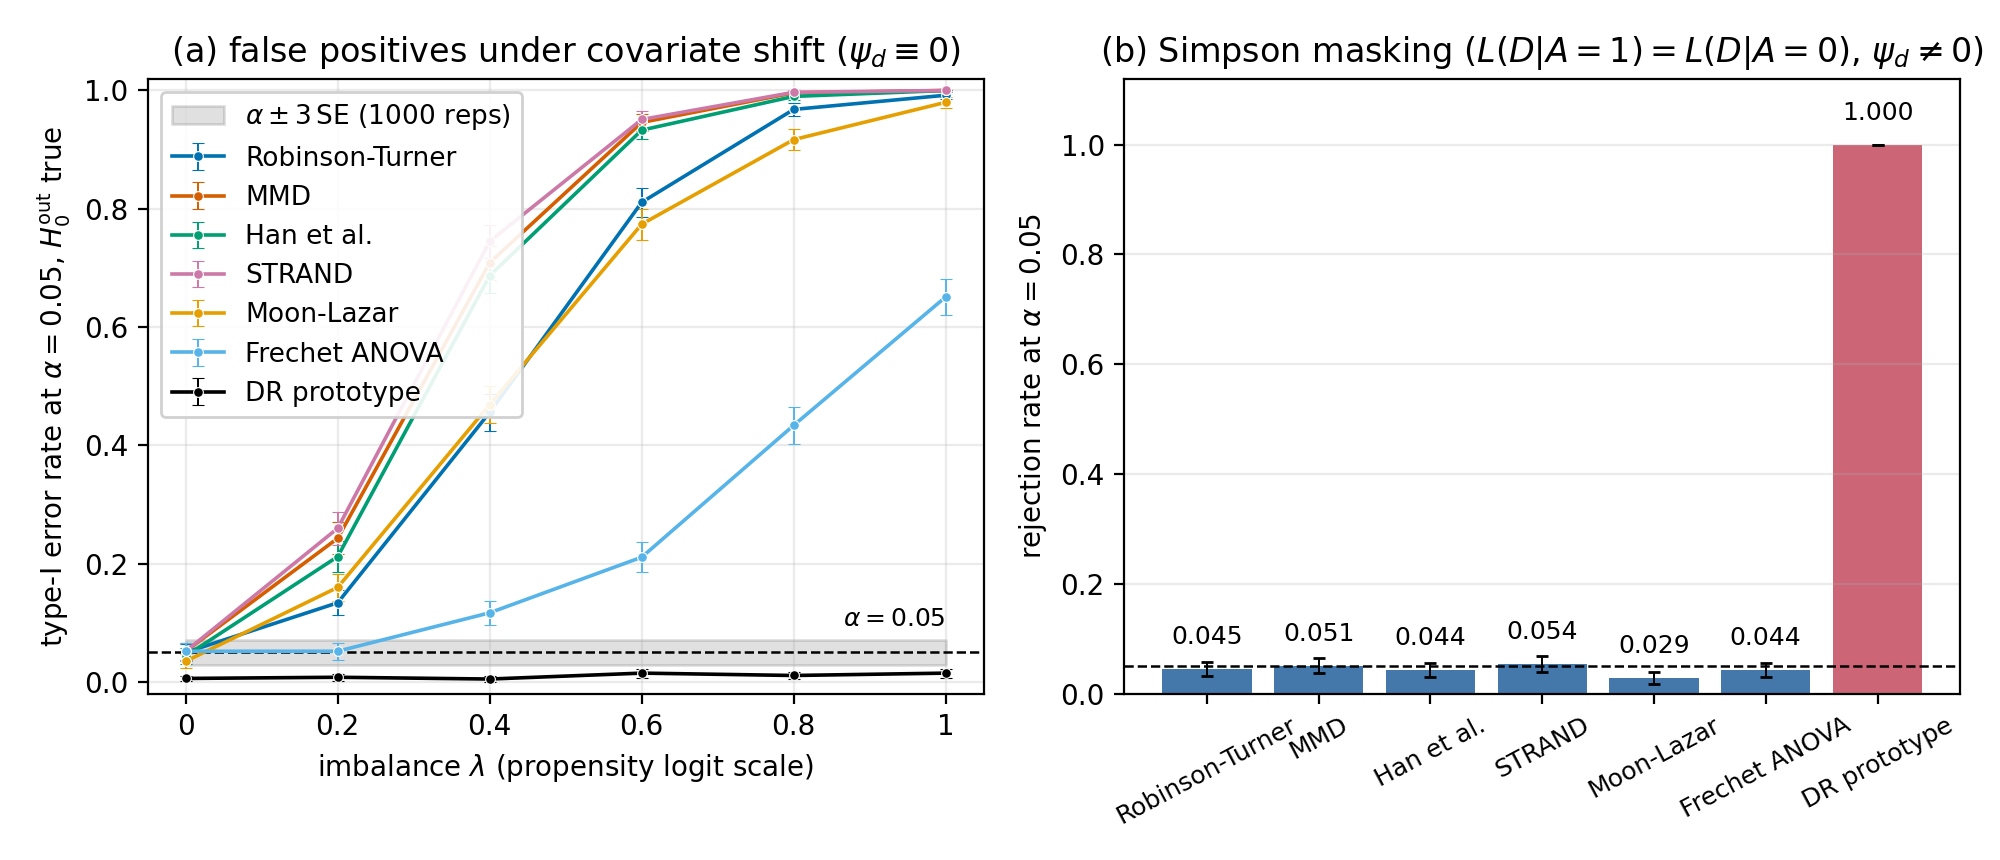
\includegraphics[width=\textwidth]{fig1_imbalance_validity.png}
\caption{Imbalance sweep with $1000$ replications per cell. Panel (a) reports rejection rates under exact causal nullity ($H_0^{\mathrm{out}}$ is true) as a function of the imbalance parameter $\lambda$ for the six tests of $H_0^{\mathrm{cond}}$ and for the adjusted outcome prototype; the band is $\alpha \pm 3$ Monte Carlo standard errors. Panel (b) reports the masking design, where $H_0^{\mathrm{cond}}$ holds exactly by construction while the standardized adjusted contrast is nonzero, so competitor rejection is their size and prototype rejection is power against $H_0^{\mathrm{out}}$.}
\label{fig:imbalance}
\end{figure}

\begin{table}[t]
\centering
\small
\setlength{\tabcolsep}{3.5pt}
\resizebox{\textwidth}{!}{%
\begin{tabular}{lccccccc}
\toprule
 & \multicolumn{6}{c}{$H_0^{\mathrm{out}}$ true, causal null, rejection rate (MC SE)} & Masking design \\
\cmidrule(lr){2-7}
\multicolumn{1}{c}{Test (null it tests)} & $\lambda=0$ & $\lambda=0.2$ & $\lambda=0.4$ & $\lambda=0.6$ & $\lambda=0.8$ & $\lambda=1.0$ & $H_0^{\mathrm{cond}}$ true \\
\midrule
\multicolumn{8}{l}{\emph{Competitors testing $H_0^{\mathrm{cond}}$}} \\
Robinson--Turner & 0.050 (0.007) & 0.134 (0.011) & 0.456 (0.016) & 0.811 (0.012) & 0.968 (0.006) & 0.992 (0.003) & 0.045 (0.007) \\
Kernel MMD & 0.052 (0.007) & 0.243 (0.014) & 0.709 (0.015) & 0.946 (0.007) & 0.996 (0.002) & 1.000 (0.000) & 0.051 (0.007) \\
Han et al. & 0.044 (0.006) & 0.212 (0.013) & 0.687 (0.015) & 0.933 (0.008) & 0.990 (0.003) & 1.000 (0.000) & 0.044 (0.006) \\
STRAND & 0.052 (0.007) & 0.260 (0.014) & 0.745 (0.014) & 0.951 (0.007) & 0.997 (0.002) & 1.000 (0.000) & 0.054 (0.007) \\
Moon--Lazar & 0.035 (0.006) & 0.160 (0.012) & 0.469 (0.016) & 0.774 (0.013) & 0.917 (0.009) & 0.980 (0.004) & 0.029 (0.005) \\
Fr\'echet ANOVA & 0.052 (0.007) & 0.052 (0.007) & 0.117 (0.010) & 0.211 (0.013) & 0.434 (0.016) & 0.651 (0.015) & 0.044 (0.006) \\
\midrule
\multicolumn{8}{l}{\emph{Adjusted outcome prototype testing $H_0^{\mathrm{out}}$}} \\
Prototype multiplier & 0.006 (0.002) & 0.008 (0.003) & 0.005 (0.002) & 0.015 (0.004) & 0.011 (0.003) & 0.015 (0.004) & 1.000 (0.000) \\
\bottomrule
\end{tabular}}
\caption{Imbalance sweep, $1000$ replications per cell, nominal $\alpha=0.05$. The first six rows test $H_0^{\mathrm{cond}}$, the conditional diagram law given covariates; the last row tests $H_0^{\mathrm{out}}$, the covariate-standardized functional mean. Under the causal null the first six rates are type-I error against a null that is false in composition, while the adjusted rate is type-I error against the target null. In the masking column, $H_0^{\mathrm{cond}}$ is true exactly and the adjusted contrast is nonzero, so the first six rates are size for their null and the adjusted rate is power against $H_0^{\mathrm{out}}$. Monte Carlo standard errors are binomial at $1000$ replications and are about $0.007$ at $\alpha=0.05$.}
\label{tab:imbalance}
\end{table}
\subsection{Outcome-level calibration}
\label{sec:exp:calibration}

The outcome-level test is calibrated on the oracle fleet ($500$ replications in each of $24$ cells) and on three cloud, learner, and stress batteries reported in the appendix. Table~\ref{tab:oracle} gives the compact cell record. Across the twelve null cells the adjusted multiplier test rejects at $0.026$ to $0.064$ and the frozen stratified permutation at $0.026$ to $0.052$; across the twelve alternative cells the ranges are $0.990$ to $1.000$ and $0.944$ to $1.000$ respectively. The largest null rate, $0.064$ at $n=50$ under the randomized regime, is a small-sample fluctuation rather than a systematic defect. Two null cells read $0.026$, one for each calibration path, at $n=500$ under the strongest imbalance for the multiplier and at $n=200$ under intermediate imbalance for the permutation. Both lie below the pre-registered $0.03$ edge but within Monte Carlo error of it; both are recorded strictly rather than rounded and remain open items, not evidence of a uniform size guarantee.

The point-cloud battery ($200$ replications per cell) reads $0.035$ (standard error $0.013$) for the multiplier and $0.025$ (standard error $0.011$) for the permutation under the same strong-imbalance null, and $0.415$ (standard error $0.035$) and $0.485$ (standard error $0.035$) on the covariate-driven alternative at $n=100$ with regime $1.0$. The learner battery ($100$ replications per learner) reads null rates of $0.03$ to $0.06$ for the multiplier and $0.03$ to $0.04$ for the permutation; the stress battery ($100$ replications per misspecification case) reads $0.00$ to $0.05$ and $0.00$ to $0.03$. A neural propensity learner at $n=200$ under the strongest imbalance gives $0.09$ to $0.10$, about one standard error ($0.029$) above the band, flagged as a learner-robustness item rather than a finding. The degree-multiplicity battery supports the same calibration layer: over $6000$ pooled replications the studentized comparator holds an empirical family-wise error rate of $0.0392$ under the frozen permutation and $0.0448$ under the shared multiplier, and it is exactly scale-invariant, whereas the unstudentized shared maximum collapses from $0.703$ to $0.053$ when one degree's silhouettes are rescaled while the studentized comparator holds $0.714$ against $0.709$. The battery carries one inherited conservative miss at $0.028$ and one finite-sample screen miss at $0.0364$ (pooled $0.0312$ across seeds), which falsifies finite-sample equality of size rather than upper control, and no finite-sample exactness is claimed.

The double-robustness stress statement is deliberately narrow. The outcome regression in the stress design is a nine-term oracle model, and the battery misspecifies the Fourier basis, the two propensity interactions, or both. Under the stress cases the adjusted null rates stay in $0.00$ to $0.05$: the both-nuisances-misspecified stress cell itself reads $0.00$ for the multiplier and $0.00$ for the permutation at $n=100$ and $100$ replications, with Monte Carlo standard errors of $0.017$ to $0.024$. The battery therefore documents insensitivity along the tested misspecification directions, not double robustness at the rate the theory assumes, and the appendix records the cells. A separate both-nuisances-misspecified robustness panel in the bake-off (Section~\ref{sec:exp:bakeoff}) is the uninformative control, at $0.080$ and $0.090$; it is a different experiment from the stress cell and is labelled as such.

\begin{table}[t]
\centering
\small
\setlength{\tabcolsep}{4pt}
\resizebox{\textwidth}{!}{%
\begin{tabular}{lcccccc}
\toprule
\multicolumn{7}{l}{\emph{$H_0^{\mathrm{out}}$ true (null cells): rejection rate (MC SE), $500$ replications per cell}} \\
\cmidrule(lr){2-7}
$n$ (total) & regime $0$ mult & regime $0$ perm & regime $0.5$ mult & regime $0.5$ perm & regime $1.0$ mult & regime $1.0$ perm \\
\midrule
$50$   & 0.064 (0.011) & 0.040 (0.009) & 0.042 (0.009) & 0.034 (0.008) & 0.044 (0.009) & 0.046 (0.009) \\
$100$  & 0.056 (0.010) & 0.038 (0.009) & 0.056 (0.010) & 0.034 (0.008) & 0.048 (0.010) & 0.052 (0.010) \\
$200$  & 0.036 (0.008) & 0.030 (0.008) & 0.038 (0.009) & 0.026 (0.007) & 0.034 (0.008) & 0.030 (0.008) \\
$500$  & 0.040 (0.009) & 0.046 (0.009) & 0.034 (0.008) & 0.030 (0.008) & 0.026 (0.007) & 0.038 (0.009) \\
\midrule
\multicolumn{7}{l}{\emph{$H_0^{\mathrm{out}}$ false (alternative cells): rejection rate (MC SE), $500$ replications per cell}} \\
\cmidrule(lr){2-7}
$n$ (total) & regime $0$ mult & regime $0$ perm & regime $0.5$ mult & regime $0.5$ perm & regime $1.0$ mult & regime $1.0$ perm \\
\midrule
$50$   & 0.992 (0.004) & 0.972 (0.007) & 0.996 (0.003) & 0.970 (0.008) & 0.990 (0.004) & 0.944 (0.010) \\
$100$  & 1.000 (0.000) & 0.994 (0.003) & 1.000 (0.000) & 0.994 (0.003) & 1.000 (0.000) & 0.974 (0.007) \\
$200$  & 1.000 (0.000) & 1.000 (0.000) & 1.000 (0.000) & 0.998 (0.002) & 1.000 (0.000) & 0.984 (0.006) \\
$500$  & 1.000 (0.000) & 1.000 (0.000) & 1.000 (0.000) & 1.000 (0.000) & 1.000 (0.000) & 0.990 (0.004) \\
\bottomrule
\end{tabular}}
\caption{Oracle calibration of the adjusted outcome test, $500$ replications per cell, nominal $\alpha=0.05$. Multiplier and frozen stratified permutation paths both test $H_0^{\mathrm{out}}$, the covariate-standardized functional mean; regime indexes the strength of covariate-driven imbalance ($0$, $0.5$, $1.0$). Null cells range from $0.026$ to $0.064$ for the multiplier and $0.026$ to $0.052$ for the permutation; the two $0.026$ cells lie one Monte Carlo step below the pre-registered $0.03$ edge and are recorded without rounding. Alternative cells range from $0.990$ to $1.000$ and $0.944$ to $1.000$. Point-cloud, learner, and stress batteries appear in the appendix.}
\label{tab:oracle}
\end{table}

\subsection{Distribution-level separation}
\label{sec:exp:separation}

The distribution-level experiment uses $300$ replications per design and sample size for $n \in \{25,50,100,200\}$ and evaluates the frozen expected-measure test against the outcome-level tests on two exact witnesses. Table~\ref{tab:witnesses} records the exact values, and Figure~\ref{fig:separation} shows the empirical separation.

The first witness, the deterministic W1, realizes $H_0^{\mathrm{out}}$ exactly at the realization level: the deterministic split leaves the mean normalized silhouette gap at machine zero, and the $300$-replication experiment reads a mean supremum gap of $1.1\times10^{-16}$ at $n=25$ and $0$ thereafter. The expected persistence measure nevertheless separates with an L1 contrast of $2.460375$, and the distribution-level permutation test rejects in $1.000$ of replications at every sample size with standard error $0.000$, as does the universal-kernel MMD (power $1.000$; squared discrepancy $1.916989$). On the same replications the outcome-level permutation test sits at $0.020$ to $0.043$, which is correct behavior because its null is true, and the outcome-level multiplier test is at $0.000$ because the AIPW scores are exactly constant on this realization-invariant statistic. That zero is a documented degenerate-conservative artefact of the multiplier null on a degenerate statistic, not a size claim, and the simulation pipeline refuses the studentized distribution-level statistic on the same witness for the same reason.

The second witness, W2', reverses the roles: the expected measure is exactly unchanged in law, with population L1 zero, while the outcome-level laws differ through a multiplicity mixture over two locations. The experiment reads distribution-level rates of $0.030$ to $0.057$, in band, while the outcome multiplier has power $0.610$ to $1.000$ and the outcome permutation $0.457$ to $1.000$ across the sample sizes. The sample L1 falls from $1.842$ at $n=25$ to $0.634$ at $n=200$; this is Monte Carlo noise around an exactly zero population value and is not a power curve. The mean silhouette gap stays near the exact value throughout, with sample values from $0.526$ to $0.549$ against the exact $0.544$.

The separation is therefore a matter of pairing, not of general topological sensitivity. Under the default normalized-silhouette and expected-measure pairing used here, the two nulls are logically independent: neither implies the other, and a rejection by one is not a rejection by the other. The universal-kernel MMD pairing is strictly stronger in the nested direction, and the same exact witnesses separate there as well, but the statement remains confined to the frozen finite grid, and equality of the unprojected persistence measures is not certified.

\begin{figure}[t]
\centering
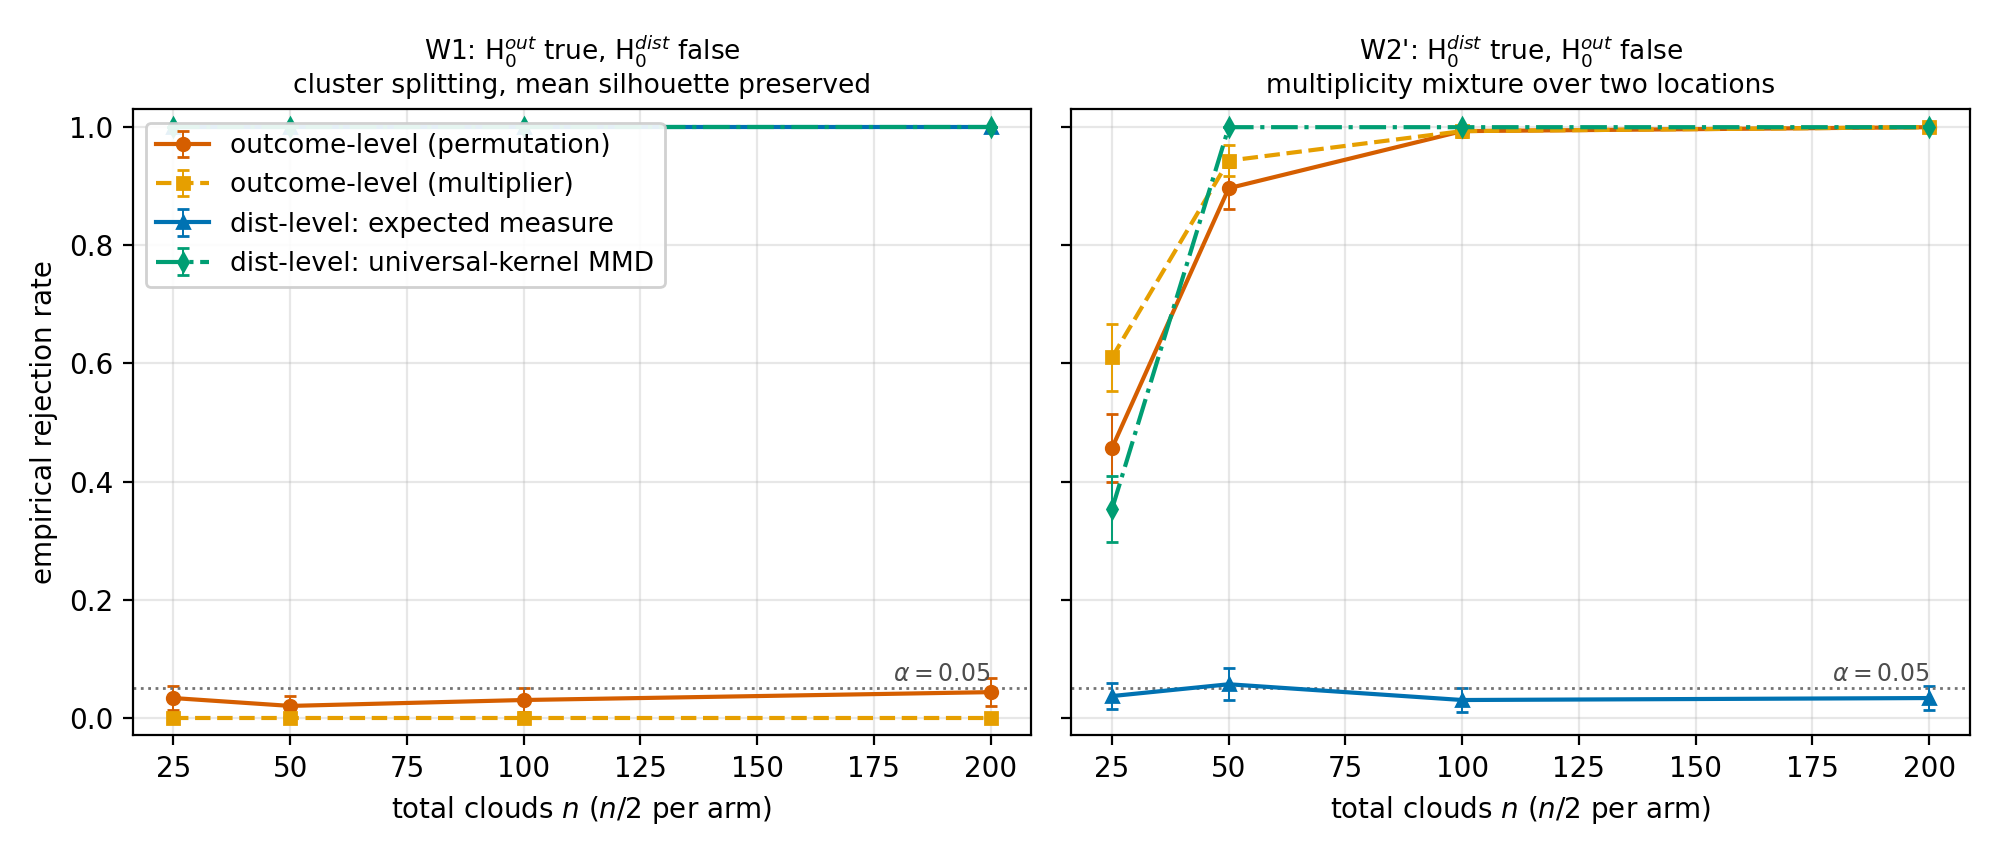
\includegraphics[width=\textwidth]{fig2_c2_separation.png}
\caption{Separation witnesses with $300$ replications per design and sample size. Left: the deterministic W1 holds $H_0^{\mathrm{out}}$ exactly while the expected persistence measure separates, so the two distribution-level procedures have power $1.000$ at every $n$ while the outcome permutation test stays near $\alpha$ and the outcome multiplier is degenerate. Right: W2' holds the expected-measure null in law while the outcome-level tests gain power; the distribution-level permutation curve stays near $\alpha$.}
\label{fig:separation}
\end{figure}

\begin{table}[t]
\centering
\footnotesize
\setlength{\tabcolsep}{4pt}
\begin{tabular}{>{\raggedright\arraybackslash}p{3.4cm}cccc}
\toprule
Witness & Mean-silhouette gap & Expected-measure L1 & Squared MMD & Balanced root-MMD \\
\midrule
W1 (split, $H_0^{\mathrm{out}}$ true exactly; $H_0^{\mathrm{dist}}$ false) & $0$ (machine zero) & $2.460375$ & $1.916989$ & n/a \\
W2' (multiplicity mixture, $H_0^{\mathrm{dist}}$ true; $H_0^{\mathrm{out}}$ false) & $0.544$ & $0$ & $0.398762$ & $0.631476$ \\
\bottomrule
\end{tabular}
\caption{Exact witness values from finitely supported laws, computed in exact arithmetic with no Monte Carlo. The pairing is the default normalized-silhouette and expected-measure pairing at weight $r=3$. W1 has the outcome-level null true exactly while the finite-grid distribution-level null is false; W2' reverses this. The two nulls are logically independent under this pairing, the MMD pairing is strictly stronger in the nested direction, and the balanced root-MMD is reported for the balanced version of W2'. The deterministic W1 here is the separation witness; the stochastic W1 power design of Section~\ref{sec:exp:weaknull} is a different, stochastic counterpart and is not used as evidence of separation.}
\label{tab:witnesses}
\end{table}
\subsection{Weak-null calibration of the distribution-level test}
\label{sec:exp:weaknull}

The distribution-level test targets $H_0^{\mathrm{dist,grid}}$, the weak expected-measure null on the frozen grid, for which the sharp null of identical unit-level laws is a strict subset. The calibration fleet uses $500$ replications per size cell and $300$ per local-power cell, the cell record is summarized below with the frozen contract described in the design subsection and printed in full, with per-cell standard errors, in Table~\ref{tab:weaknull} of the appendix, and Figure~\ref{fig:calibration} shows the size and power curves. W2' and confounded $r=0$ cells are in band at every sample size, reading $0.042$ to $0.070$ and $0.046$ to $0.076$; the intermediate-confounding cells range from $0.050$ to $0.094$.

The strict pre-registered gate, which applies to the gating cells with $n \ge 200$, fails in exactly one cell: under strong confounding ($r=1.0$) at $n=200$ the studentized max-$t$ rejects at $0.096$ with a standard error of $0.013$, about $1.2$ standard errors above the upper edge of the band. The same design reads $0.066$ at $n=500$, and the remaining strong-confounding cells read $0.154$ at $n=50$ and $0.090$ at $n=100$. The matching sharp null is in band from $n=100$ onward ($0.056$, $0.072$, $0.058$) and reads $0.118$ at $n=50$. The operating recommendation is therefore differentiated: $n \ge 500$ under the strongest tested confounding, and $n \ge 200$ for the other tested weak-null designs, with no claim of finite-sample or uniform weak-null control. Power against the stochastic W1 power design is $0.996$ at $n=50$ and $1.000$ at $n \ge 100$, and the local-mixture curve rises from $0.033$ at weight $0$ to $0.380$, $0.997$, and $1.000$ at weights $0.25$, $0.5$, and $0.75$, so the size qualification is not a blanket loss of power.

The frozen relabeling diagnostics are reported as diagnostics only. Under strong confounding at $r=1.0$ the frozen label permutation rejects at $0.198$, $0.208$, $0.220$, and $0.228$ at $n=50$ through $500$, and the studentized stratified permutation at $0.228$, $0.244$, $0.214$, and $0.248$; these rates are witnesses that the exchangeability law of the relabeling does not match the weak-null sampling law when nuisances are frozen, and they are not size claims. Under the sharp null the permutation and multiplier paths agree empirically from $n=100$ onward, which supports the permutation as a diagnostic while the studentized multiplier remains the production calibration, empirically only and without an exact finite-sample guarantee. The Rademacher multiplier path reads $0.106$ against the Gaussian path's $0.056$ at $n=50$ and is retained as a diagnostic rather than treated as interchangeable with the Gaussian multiplier.

\begin{center}
\small
\setlength{\tabcolsep}{5pt}
\begin{tabular}{lcccc}
\toprule
\multicolumn{5}{@{}p{15.3cm}@{}}{\textbf{Weak-null cell record, null tested: $H_0^{\mathrm{dist,grid}}$, rate (MC SE), $500$ replications per cell, band $[0.03,0.08]$}} \\
\midrule
Design & $n=50$ & $n=100$ & $n=200$ & $n=500$ \\
\midrule
W2' (no covariates) & 0.056 (0.010) & 0.058 (0.011) & 0.070 (0.011) & 0.042 (0.009) \\
Confounded $r=0.0$ & 0.076 (0.012) & 0.046 (0.009) & 0.054 (0.010) & 0.058 (0.011) \\
Confounded $r=0.5$ & 0.094 (0.013) & 0.058 (0.011) & 0.050 (0.010) & 0.050 (0.010) \\
Confounded $r=1.0$ & 0.154 (0.016) & 0.090 (0.013) & \textbf{0.096 (0.013)} & 0.066 (0.011) \\
Sharp null, $r=1.0$ & 0.118 (0.014) & 0.056 (0.010) & 0.072 (0.012) & 0.058 (0.011) \\
\midrule
\multicolumn{5}{@{}p{15.3cm}@{}}{\emph{Frozen permutation diagnostic, $r=1.0$: 0.198 (0.018), 0.208 (0.018), 0.220 (0.019), 0.228 (0.019); diagnostic only}} \\
\multicolumn{5}{@{}p{15.3cm}@{}}{\emph{Stratified permutation diagnostic, $r=1.0$: 0.228 (0.019), 0.244 (0.019), 0.214 (0.018), 0.248 (0.019); diagnostic only}} \\
\midrule
\multicolumn{5}{@{}p{15.3cm}@{}}{Power against stochastic W1 ($H_0^{\mathrm{dist,grid}}$ false): 0.996 at $n=50$, 1.000 at $n \ge 100$ (MC SE $\le 0.003$)} \\
\multicolumn{5}{@{}p{15.3cm}@{}}{Local mixture at $n=200$ ($300$ replications per cell): 0.033, 0.380, 0.997, 1.000, 1.000 at weights $0,0.25,0.5,0.75,1.0$ (MC SE $\le 0.028$)} \\
\midrule
\multicolumn{5}{@{}p{15.3cm}@{}}{\emph{The bold entry is the single strict-gate failure; the same strong-confounding design is in band at $n=500$ ($0.066$).}} \\
\multicolumn{5}{@{}p{15.3cm}@{}}{\emph{The sharp-null rows are a strict subset of $H_0^{\mathrm{dist,grid}}$; the permutation rows are exchangeability-failure witnesses and carry no size claim.}} \\
\bottomrule
\end{tabular}
\end{center}

\begin{figure}[t]
\centering
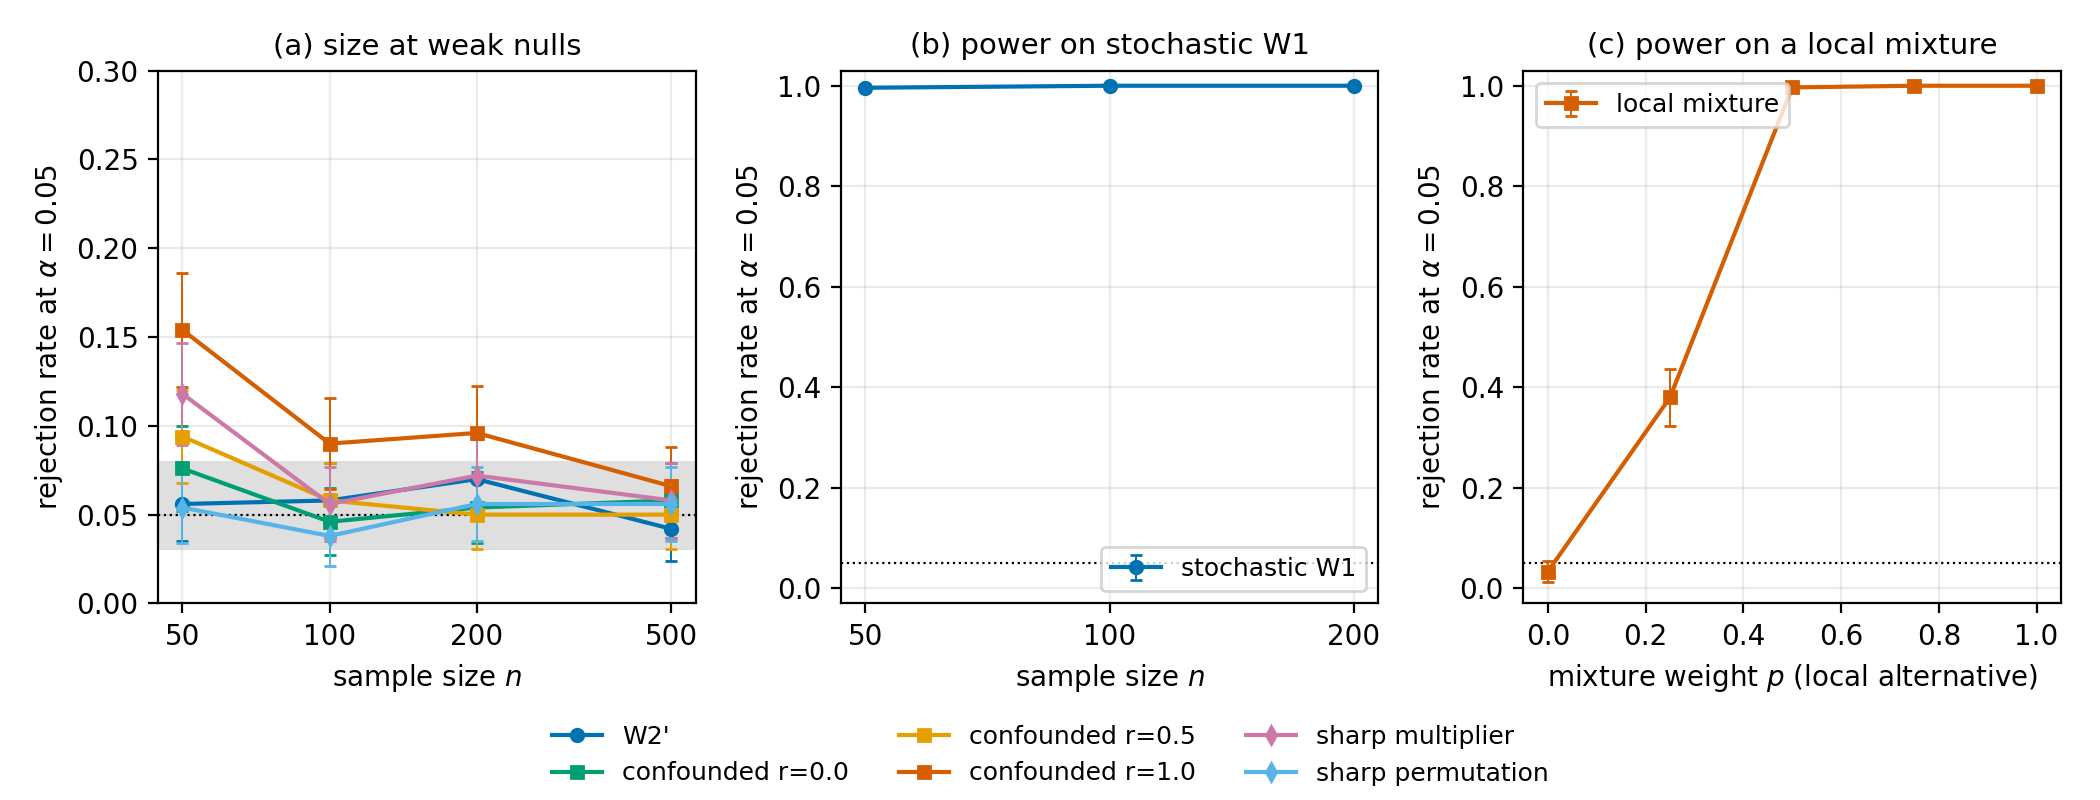
\includegraphics[width=\textwidth]{fig3_calibration_scope.png}
\caption{Weak-null calibration of the distribution-level test, nominal $\alpha=0.05$. Panel (a) shows size under the weak expected-measure null $H_0^{\mathrm{dist,grid}}$ for the tested designs and sample sizes; the shaded band is the pre-registered $[0.03,0.08]$ region. Panel (b) shows power against the stochastic W1 power design (a stochastic counterpart of the deterministic separation witness), and panel (c) shows power on the local mixture as the mixture weight varies. The bold cell in the cell record, strong confounding at $n=200$ ($0.096$), is visible as the upper excursion of the strongest-confounding curve; the same design is in band at $n=500$.}
\label{fig:calibration}
\end{figure}

\subsection{Replicated-cloud bake-off}
\label{sec:exp:bakeoff}

The bake-off evaluates all procedures on the replicated-cloud panel across five alternative families plus a no-effect panel, three imbalance levels, and $n \in \{50,100,200\}$ at $100$ replications per cell, with $500$-replication tightenings on four decision-relevant cells. Table~\ref{tab:bakeoff-size} reports size at $n=200$ under randomization and under strong imbalance; Figure~\ref{fig:bakeoff} shows the full grid; Table~\ref{tab:winslosses} records the named wins and losses.

Under randomization every procedure holds size at $n=200$, with rates between $0.020$ and $0.070$. Under strong imbalance the six $H_0^{\mathrm{cond}}$ tests reject at $0.430$ (Fr\'echet ANOVA) to $0.950$ (kernel MMD and Han et al.), whereas the adjusted outcome multiplier reads $0.030$ (standard error $0.017$), the frozen permutation $0.000$, the distribution-level max-$t$ $0.060$ (standard error $0.024$), and the distribution-level MMD $0.020$ (standard error $0.014$). This reproduces the imbalance sweep's false-positive finding inside the bake-off. Two flags are reported: the outcome multiplier reads $0.120$ (standard error $0.032$) at strong imbalance and $n=100$, about one standard error above the band and consistent with the small-sample strong-confounding wobble of the distribution-level calibration, and the frozen permutation reads $0.000$ at strong imbalance and $n=200$, which is conservative, not anti-conservative.

The losses come first. At small $n$ and under randomization the adjusted outcome tests lose to the unadjusted procedures on a gross mean shift: at $n=50$ the outcome multiplier reads $0.110$ (standard error $0.031$) and the permutation $0.090$ (standard error $0.029$) against $0.800$ for Robinson--Turner and $1.000$ for STRAND, kernel MMD, and Han et al.; at $n=100$ the outcome multiplier reads $0.450$ (standard error $0.050$) against $1.000$ for the same group. The full-stage tightenings confirm the losses under confounding: the outcome multiplier reads $0.212$ (standard error $0.018$) at strong imbalance and $n=50$ and $0.332$ (standard error $0.021$) at $n=100$, against $0.900$ and $0.996$ for STRAND. Under confounding those competitor rates mix signal with size distortion and are not like-for-like power; they are reported descriptively. The permutation path additionally trails the multiplier under strong confounding, reading $0.360$ (standard error $0.048$) against $0.760$ (standard error $0.043$) at $n=200$, and it remains the conservative second calibration rather than the primary one. Han et al.\ win their turf on the faint rare-feature signal under mild confounding at $n=200$, reading $0.890$ (standard error $0.031$) against $0.390$ (standard error $0.049$) for the outcome multiplier, and the paper does not claim to beat the minimax-optimal intensity test on a faint intensity signal.

The wins are equally specific. The distribution-level max-$t$ is the most uniformly powerful of the distribution-level readouts on this panel: it reads $0.998$ to $1.000$ on the stochastic-split family, $1.000$ on the dispersion family, and $1.000$ on the mean-shift family at $n=200$, and $0.770$ to $0.940$ on the rare-feature family at $n=200$. On the deterministic separation witness the studentized max-$t$ is undefined because the AIPW scores are exactly constant, and the simulation pipeline correctly refuses it; the defined distribution-level readouts there are the L1 diagnostic and the kernel MMD, both $1.000$. On the rare-feature signal under randomization at $n=200$ it reads $0.940$ (standard error $0.024$) and the outcome tests read $0.530$ (standard error $0.050$) and $0.480$ (standard error $0.050$), against $0.400$ (standard error $0.049$) for the best $H_0^{\mathrm{cond}}$ competitor, Robinson--Turner. The secondary distribution-level MMD is blind to the rare feature, reading $0.020$ to $0.070$ across the grid (the largest value occurs under mild confounding at $n=100$), and is reported as a secondary-method loss rather than a failure of the distribution-level target. On the dispersion family Krebs--Rademacher holds its own target at $0.930$ (standard error $0.026$) at $n=50$ and $1.000$ (standard error $0.000$) at $n=200$, while STRAND is weak on the same alternative at $0.090$ (standard error $0.029$) and $0.230$ (standard error $0.042$); symmetrically, STRAND is blind to the deterministic split at $0.000$ where the $H_0^{\mathrm{cond}}$ tests fire at $1.000$ for their own null. The deterministic witness also isolates the separation the paper is built on: with $H_0^{\mathrm{out}}$ true, the frozen outcome permutation holds $0.040$ (standard error $0.020$) at $n=200$ and $0.010$ (standard error $0.010$) at $n=500$, the outcome multiplier reads $0.000$, and the L1 diagnostic and kernel MMD read $1.000$. The stochastic-split column saturates for all procedures except the outcome permutation at strong imbalance and $n=200$, where the full-stage record reads $0.746$ (standard error $0.019$) against $0.972$ (standard error $0.007$) for the multiplier.

The equivalence declaration is scoped rather than general. Under the null at $n=200$ it declares equivalence at $0.970$ (standard error $0.017$) under randomization, $0.890$ (standard error $0.031$) under mild imbalance, and $0.650$ (standard error $0.048$) under strong imbalance, and at $n=50$ it reads $0.000$ to $0.010$ because the margin of $0.25$ is unreachable at that sample size. It therefore supports a sameness certification only at $n \ge 200$ under randomization or mild imbalance, never at $n=50$ and not under strong confounding.

Cost and memory are measured, not modelled. At $n=200$ the mean per-replication wall time is $17.5$ seconds for Han et al., $10.9$ seconds for Robinson--Turner, and $48.6$ seconds for the distribution-level MMD, while the adjusted outcome cross-fit costs $11.2$ to $11.7$ seconds and is flat over $n=50$ to $200$ because the silhouette regression dominates. Every calibration step after the fits is on the order of milliseconds, with the distribution-level max-$t$ calibration at $0.66$ seconds. A single sequential replication at $n=200$ peaks at $1548$ megabytes of resident memory and runs in $48.95$ seconds. Those measurements are why coarse $n=500$ coverage for the full loops-cloud families was deferred (about $284$ seconds per replication sequential, an estimated $8$ to $11$ hours at sixteen workers) and why the strong-imbalance mean-shift cell at $n=200$ was deferred as a run of over two hours; the only $n=500$ bake-off evidence is the deterministic-witness pilot, and this coverage limit is not repaired by any claim.

The robustness panel ($100$ replications, $n=100$) reports four design perturbations under the null. Uniform outliers on $10\%$ of units leave every procedure in band, with the adjusted outcome multiplier at $0.090$ (standard error $0.029$), the permutation at $0.040$ (standard error $0.020$), and the distribution-level max-$t$ at $0.020$ (standard error $0.014$) against $H_0^{\mathrm{cond}}$ rates of $0.040$ to $0.090$. Heavy-tailed loop counts leave every procedure in band with rates at or below $0.040$. Arm-confounded cloud cardinality, by contrast, rejects at $1.000$ in every column including the adjusted and distribution-level procedures: cloud cardinality is itself part of the diagram signal, so an arm-confounded point count is a confounded contrast rather than power, and the design instruction is to equalise it or treat size as part of the treatment. The both-nuisances-misspecified control at $n=100$ leaves the adjusted procedures at $0.080$ and $0.090$ and fails to separate them from luck; it is reported as an uninformative negative control, not as evidence for or against the adjustment. This panel is distinct from the outcome-level stress battery's both-misspecified cell, which reads $0.00$ (multiplier) and $0.00$ (permutation) at $n=100$.

\begin{figure}[t]
\centering
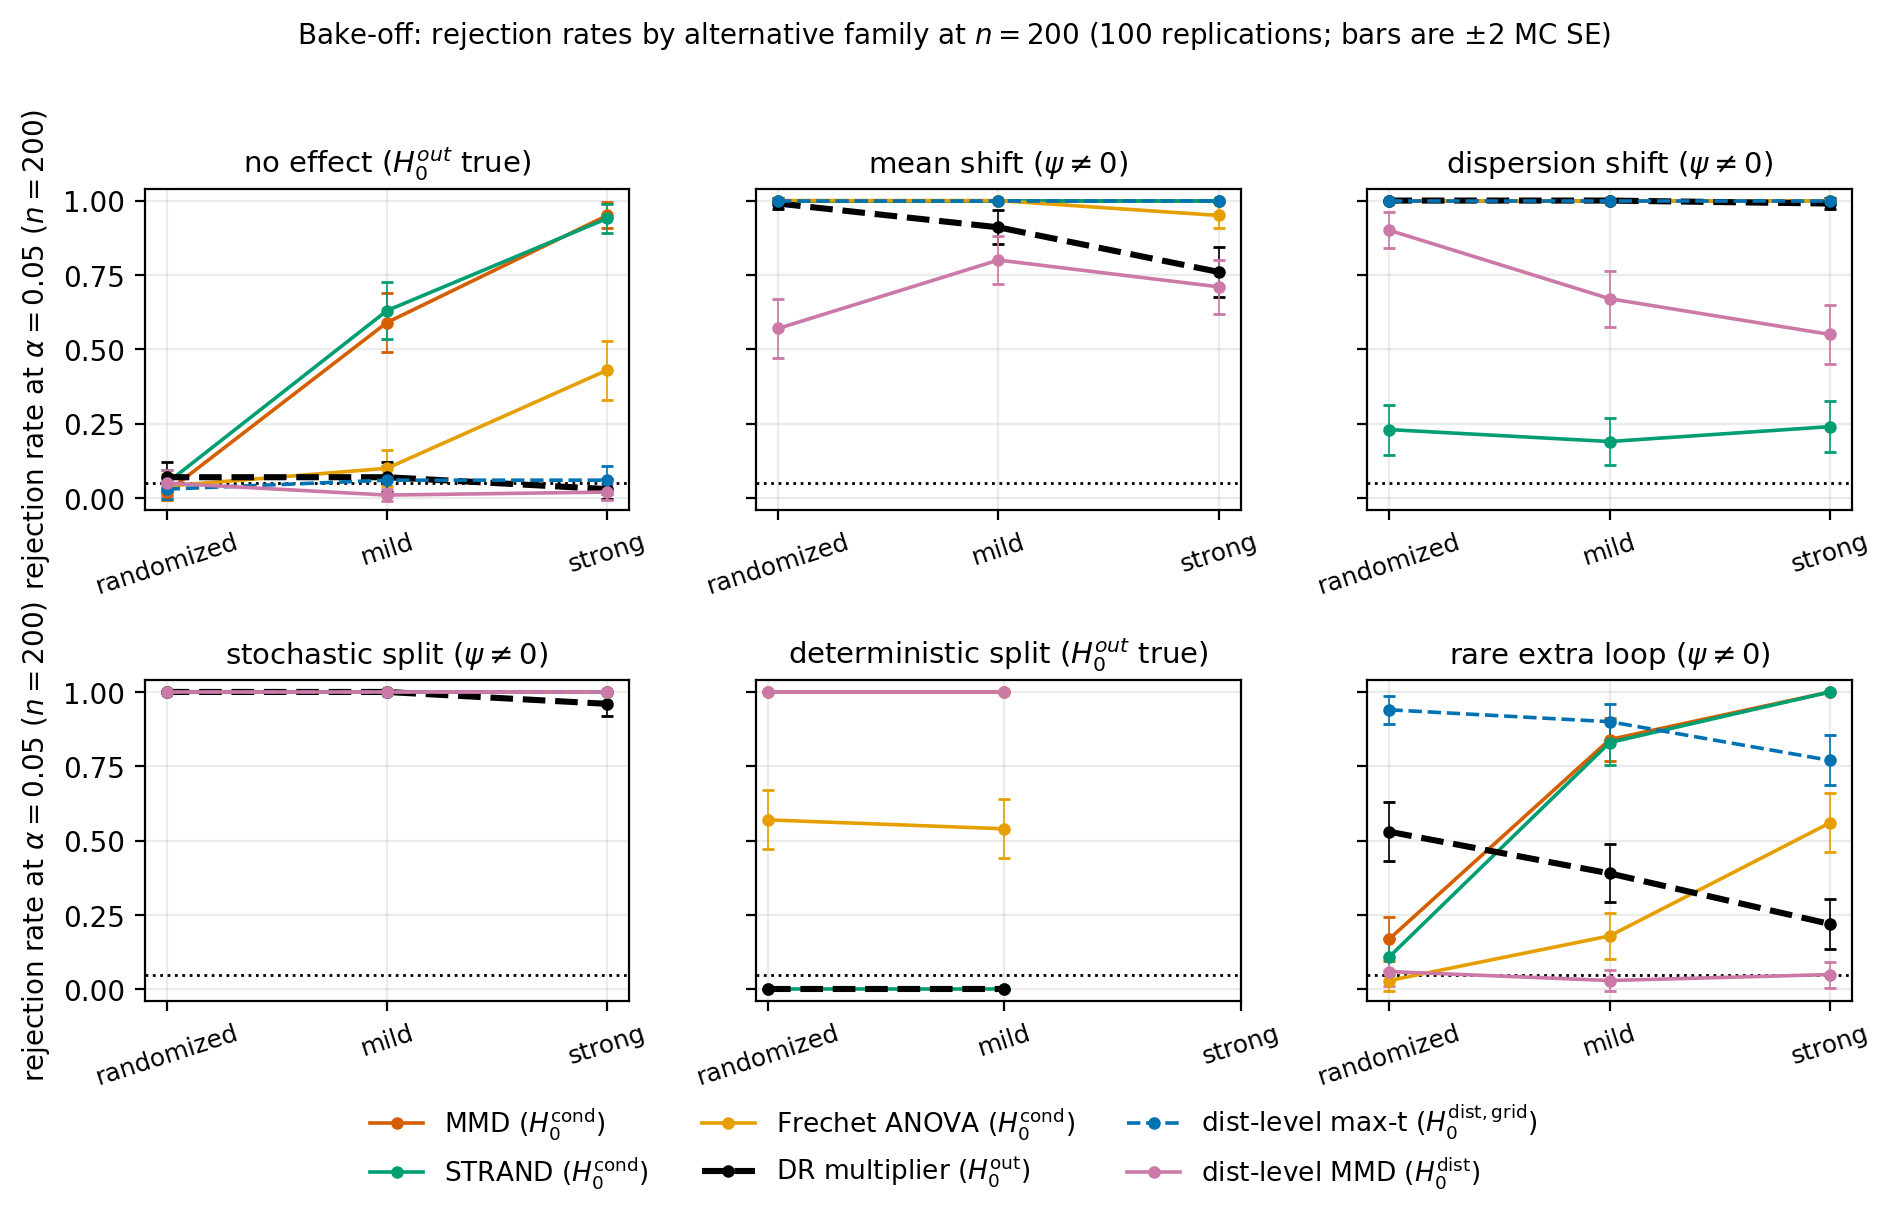
\includegraphics[width=\textwidth]{fig4_bakeoff.png}
\caption{Bake-off rejection rates at $n=200$ by alternative family and imbalance strength, with $100$ replications and bars of $\pm 2$ Monte Carlo standard errors. The null tested by each curve is printed in the legend and in the panel titles: the outcome multiplier tests $H_0^{\mathrm{out}}$, the distribution-level max-$t$ and MMD test the two distribution-level nulls, and the unadjusted curves test $H_0^{\mathrm{cond}}$. Under strong imbalance the unadjusted curves on the no-effect panel measure size distortion, not power.}
\label{fig:bakeoff}
\end{figure}

\begin{table}[H]
\centering
\small
\setlength{\tabcolsep}{3pt}
\begin{tabular}{>{\raggedright\arraybackslash}p{2.0cm}>{\raggedright\arraybackslash}p{5.6cm}cc}
\toprule
Null tested & Procedure & Randomized ($\lambda=0$) & Strong imbalance ($\lambda=1.0$) \\
\midrule
$H_0^{\mathrm{cond}}$ & Robinson--Turner & 0.040 (0.020) & 0.840 (0.037) \\
$H_0^{\mathrm{cond}}$ & Kernel MMD & 0.020 (0.014) & 0.950 (0.022) \\
$H_0^{\mathrm{cond}}$ & Han et al. & 0.030 (0.017) & 0.950 (0.022) \\
$H_0^{\mathrm{cond}}$ & STRAND & 0.050 (0.022) & 0.940 (0.024) \\
$H_0^{\mathrm{cond}}$ & Moon--Lazar & 0.040 (0.020) & 0.700 (0.046) \\
$H_0^{\mathrm{cond}}$ & Fr\'echet ANOVA & 0.040 (0.020) & 0.430 (0.050) \\
\midrule
$H_0^{\mathrm{disp}}$ & Krebs--Rademacher & 0.020 (0.014) & 0.180 (0.038) \\
\midrule
$H_0^{\mathrm{out}}$ & Outcome multiplier & 0.070 (0.026) & 0.030 (0.017) \\
$H_0^{\mathrm{out}}$ & Outcome permutation & 0.060 (0.024) & 0.000 (0.000) \\
$H_0^{\mathrm{dist,grid}}$ & Distribution-level max-$t$ & 0.030 (0.017) & 0.060 (0.024) \\
$H_0^{\mathrm{dist}}$ (kernel) & Distribution-level MMD & 0.050 (0.022) & 0.020 (0.014) \\
\midrule
$H_0^{\mathrm{equiv}}$ & Equivalence declaration (rejection declares equivalence) & 0.970 (0.017) & 0.650 (0.048) \\
\bottomrule
\end{tabular}
\caption{Null-family size in the bake-off at $n=200$, $100$ replications per cell, nominal $\alpha=0.05$. Each row names the null it tests. Under randomization all procedures hold size because $H_0^{\mathrm{cond}}$ implies $H_0^{\mathrm{out}}$ there (the converse fails in general); under strong imbalance the six $H_0^{\mathrm{cond}}$ rows measure rejection of a conditional null that is false in composition, while the adjusted and distribution-level rows measure size against their own targets. The permutation row is conservative, not anti-conservative; the equivalence row is a declaration rate under the non-equivalence null, so higher is sameness, not type-I error. The Krebs--Rademacher row tests $H_0^{\mathrm{disp}}$, equality of the arm-conditional loop-count (dispersion) laws.}
\label{tab:bakeoff-size}
\end{table}
\begin{table}[H]
\centering
\small
\setlength{\tabcolsep}{3.5pt}
\begin{tabular}{p{3.6cm}p{1.0cm}p{3.9cm}p{3.6cm}p{2.6cm}}
\toprule
Setting (null tested) & Reps & Target procedure(s), rate (SE) & Named comparator(s), rate (SE) & Read \\
\midrule
Mean shift, randomized, $n=50$ ($H_0^{\mathrm{cond}}\Rightarrow H_0^{\mathrm{out}}$) & 100 & multiplier 0.110 (0.031); permutation 0.090 (0.029) & RT 0.800 (0.040); STRAND, MMD, Han 1.000 (0.000) & Loss at small $n$ \\
Mean shift, randomized, $n=100$ & 100 & multiplier 0.450 (0.050); permutation 0.280 (0.045) & same group 1.000 (0.000) & Loss at small $n$ \\
Mean shift, strong, $n=50$ & 500 & multiplier 0.212 (0.018); permutation 0.120 (0.015) & STRAND 0.900 (0.013); Han 0.802 (0.018) & Loss, descriptive under confounding \\
Mean shift, strong, $n=100$ & 500 & multiplier 0.332 (0.021); permutation 0.144 (0.016) & STRAND 0.996 (0.003); Han 0.992 (0.004) & Loss, descriptive under confounding \\
Mean shift, randomized, $n=200$ & 100 & multiplier 0.990 (0.010); max-$t$ 1.000 (0.000) & $H_0^{\mathrm{cond}}$ group 1.000 (0.000) & Catch-up at $n=200$ \\
Dispersion, randomized, $n=50$ and $n=200$ & 100 & max-$t$ 1.000 (0.000); multiplier 0.970 (0.017) at $n=50$, 1.000 (0.000) at $n=200$ & KR 0.930 (0.026), 1.000 (0.000, own dispersion null); STRAND 0.090 (0.029), 0.230 (0.042) & KR holds its turf; STRAND weak \\
Stochastic split, strong, $n=200$ (full stage) & 500 & max-$t$ 0.998 (0.002); multiplier 0.972 (0.007); permutation 0.746 (0.019) & $H_0^{\mathrm{cond}}$ group 1.000 (0.000) & Permutation trails the multiplier \\
Deterministic split, randomized, $n=200$ ($H_0^{\mathrm{out}}$ true) & 100 & permutation 0.040 (0.020); multiplier 0.000 (0.000); distribution-level L1 diagnostic and kernel MMD 1.000 (0.000) & STRAND 0.000 (0.000); RT, kernel MMD, Han, Moon 1.000 (0.000) for $H_0^{\mathrm{cond}}$; Fr\'echet 0.570 (0.050) & Separation; STRAND blind; max-$t$ undefined \\
Rare feature, randomized, $n=200$ & 100 & max-$t$ 0.940 (0.024); multiplier 0.530 (0.050); permutation 0.480 (0.050) & best $H_0^{\mathrm{cond}}$, RT 0.400 (0.049); dist-level MMD 0.060 (0.024) & Win on subtle signal; secondary MMD blind \\
Rare feature, mild, $n=200$ & 100 & multiplier 0.390 (0.049); permutation 0.380 (0.049) & Han 0.890 (0.031) & Han wins its turf \\
Equivalence, $n=200$ (and $n=50$) & 100 & declaration 0.970 (0.017) randomized, 0.890 (0.031) mild, 0.650 (0.048) strong; 0.000 to 0.010 at $n=50$ & none & Scope: $n \ge 200$ randomized or mild only \\
\bottomrule
\end{tabular}
\caption{Named wins and losses in the bake-off. Every row names the null tested. Randomized rows are target-matched because $H_0^{\mathrm{cond}}$ implies $H_0^{\mathrm{out}}$ there and the converse fails in general; confounded rows are descriptive, their comparator rates mixing signal with size distortion (Table~\ref{tab:bakeoff-size}), and are not cross-null efficiency statements. Rows flagged ``full stage'' print the $500$-replication tightened estimate with its Monte Carlo standard error, which replaces the coarse $100$-replication estimate. On the deterministic split the studentized max-$t$ is undefined because the AIPW scores are exactly constant, and the distribution-level readouts there are the L1 diagnostic and the kernel MMD. The deterministic-split row is separation evidence: the outcome null holds while the distribution-level target moves, so the unadjusted rejections are correct for their own conditional null. ``Declaration'' is the equivalence rejection rate under the non-equivalence null, so higher is a sameness statement.}
\label{tab:winslosses}
\end{table}

\subsection{Local-power record}
\label{sec:exp:localpower}

The local-power program is reported with its recorded pre-registered mismatch intact. The oracle harness uses a Pitman shift of order $n^{-1/2}g$ for three shift directions (a mean shift, a bump shift, and a frequency shift), crossed with a prognostic and a non-prognostic nuisance variant (prognostic means the outcome regression depends on the covariates; the non-prognostic variant removes that dependence), at $n \in \{100,200,500\}$, with $300$ replications in each core cell and a pre-registered tolerance of $0.06$ on the gap between the empirical rate and a Gaussian-shift prediction from the pooled centered-score covariance ($20{,}000$ draws). Figure~\ref{fig:localpower} shows the empirical and predicted curves, and Table~\ref{tab:localpower} records every criterion.

At $n=500$ five of the six adjusted cells match the naive prediction within $0.06$: the non-prognostic mean cell reads $0.623$ against $0.628$, bump $0.397$ against $0.410$, and frequency $0.917$ against $0.867$; the prognostic mean reads $0.410$ against $0.450$ and bump $0.277$ against $0.285$. The prognostic frequency cell misses at $0.730$ against $0.628$, a gap of $+0.102$ with a Monte Carlo standard error of $0.026$, and this is the recorded headline mismatch. A separate valid-regime cell on the unadjusted statistic misses marginally at $+0.064$ on a partial run, and the null cells at $n=200$ confirm the predicted bias break. A completed full-fleet validator, which scores only the naive prediction, records $51$ scored rows, $9$ over the $0.06$ tolerance, $17$ beyond two standard errors, a maximum absolute gap of $0.275$, and a verdict of \texttt{confirmed=false}. The pre-registered gate therefore remains failed, and no sentence in this paper describes the local-power program as numerically confirmed.

A finite-sample correction has been derived and is reported separately, with its limits. The mechanism is an out-of-span truncation of the drift times an estimated propensity mean ratio, $g_{\mathrm{eff}} = g + \kappa_n\,(g - P_K g)$, with the basis enlarged to seven Fourier terms. The mechanism experiment removes the out-of-span fraction ($0.998$ to $0$), returns the projected score to the oracle value ($5.01$ against $4.99$), and moves the headline gap from $+0.102$ to $-0.053$, with other corrected gaps of $-0.019$, $-0.041$, $-0.022$, and $-0.043$; an $n=100$ frequency edge reads $+0.068$ and a stress setting at triple propensity scale reads $+0.157$. The correction is a finite-n expansion, not an asymptotic theorem, its mean-ratio rate is not proved, and the full-fleet validator does not apply it. The exact-ARE design record completes the picture: under the non-prognostic design the adjusted power sits below the unadjusted test at $n=200$ ($0.563$ against $0.753$) and $n=500$ ($0.567$ against $0.707$), with mean gaps of $0.14$ to $0.19$, so the asymptotic efficiency statement does not translate into finite-sample power parity. That record is reported as open, not validated.

\begin{figure}[t]
\centering
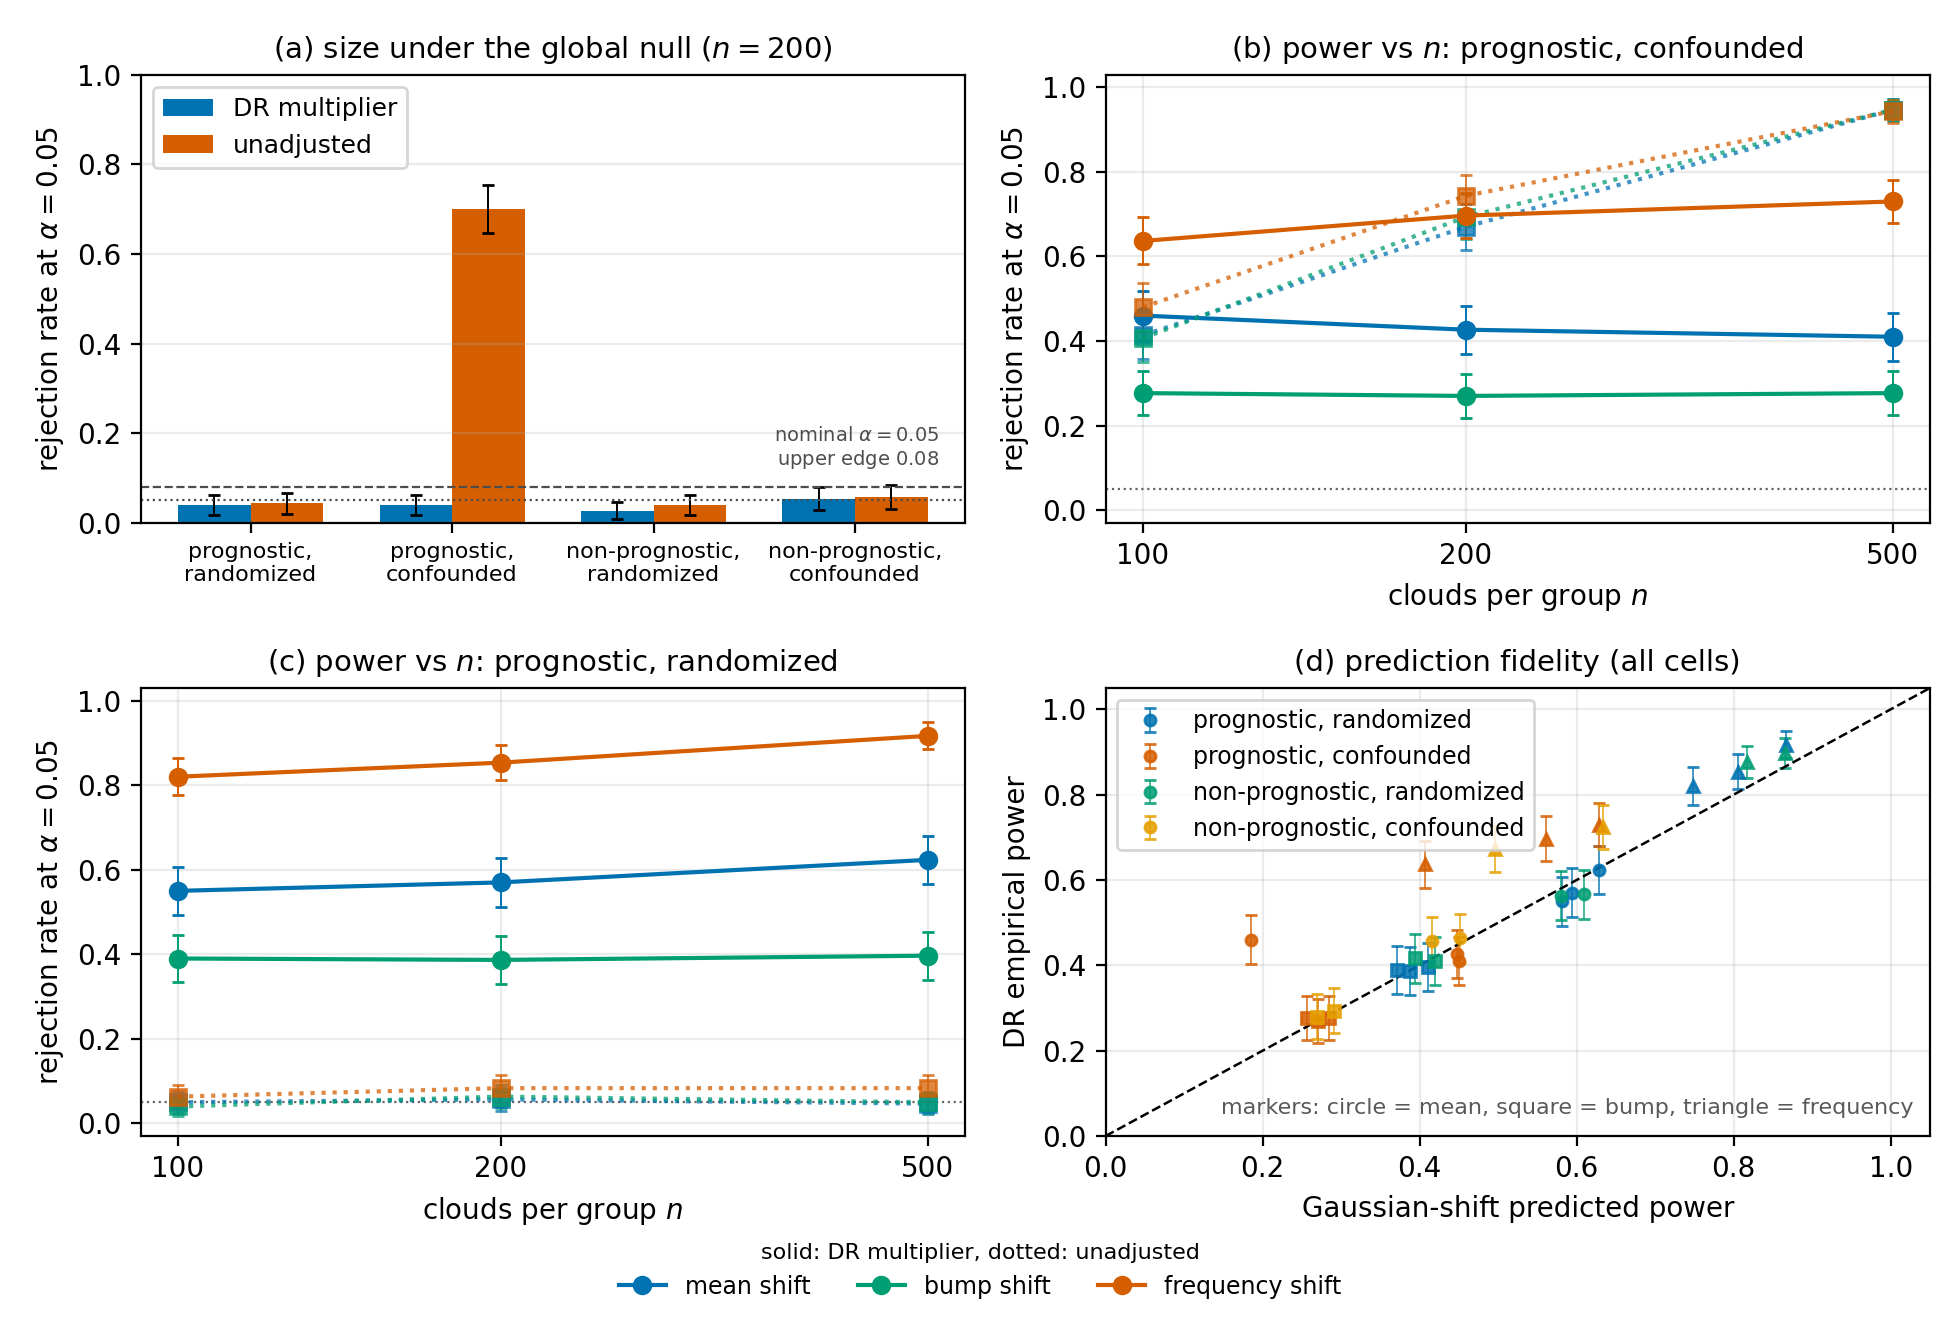
\includegraphics[width=\textwidth]{fig5_local_power.png}
\caption{Local-power record. Panel (a) shows size under the global null at $n=200$. Panel (b) shows power against sample size for the prognostic, confounded variant, with the adjusted multiplier and the unadjusted statistic along with their Gaussian-shift predictions. Panel (c) shows the prognostic, randomized variant, and panel (d) plots empirical against predicted power for all cells, where the visible departures from the diagonal include the recorded mismatch. The null tested is $H_0^{\mathrm{out}}$ for the adjusted statistic and the corresponding unadjusted null for the baseline.}
\label{fig:localpower}
\end{figure}

\clearpage
\begin{table}[H]
\centering
\small
\setlength{\tabcolsep}{3pt}
\begin{tabular}{>{\raggedright\arraybackslash}p{3.1cm}>{\raggedright\arraybackslash}p{2.7cm}>{\raggedright\arraybackslash}p{4.0cm}>{\raggedright\arraybackslash}p{2.9cm}>{\raggedright\arraybackslash}p{1.9cm}}
\toprule
Criterion (scope, null) & Pre-registered rule & Recorded outcome & Corrected outcome & Status \\
\midrule
Naive Gaussian-shift screen, six core cells at $n=500$ ($H_0^{\mathrm{out}}$) & all six within $0.06$ & five within; prognostic frequency $0.730$ against $0.628$, gap $+0.102$ ($300$ reps, MC SE $0.026$) & corrected prediction $0.783$, gap $-0.053$ (mean-ratio estimate $0.138$, probe SE $0.021$ to $0.034$) & Pre-registered rule fails; corrected rule passes \\
Completed full fleet, all scored rows ($H_0^{\mathrm{out}}$) & flag at $2$ SE or $0.06$ & $51$ scored, $9$ over $0.06$, $17$ beyond $2$ SE, max $|$gap$|$ $0.275$ & correction not applied by the validator & \texttt{confirmed=}\allowbreak\texttt{false} \\
Truncation mechanism, basis enlarged to $K=7$ ($H_0^{\mathrm{out}}$) & remove the out-of-span fraction & fraction $0.998$ to $0$; projection $5.01$ against oracle $4.99$ & not applicable & Finite-n expansion; mean-ratio rate unproved \\
Exact-ARE design, non-prognostic cells at $n=200$ and $n=500$ ($H_0^{\mathrm{out}}$) & parity with the unadjusted test under ARE $=1$ & adjusted $0.563$ against $0.753$ at $n=200$; $0.567$ against $0.707$ at $n=500$; mean gaps $0.14$ to $0.19$ ($300$ reps, MC SE $0.028$ to $0.029$) & not applicable & Open; no numerical confirmation claimed \\
\bottomrule
\end{tabular}
\caption{Local-power criterion record. The pre-registered criteria and the post-hoc corrected expansion are reported side by side under their own labels; the completed-fleet validator scores only the naive prediction, so its verdict and the corrected-gap calculation answer different questions. The null tested is $H_0^{\mathrm{out}}$ in every row, with the unadjusted baseline defined by the comparison statistic's own null. No entry supports the wording ``numerically confirmed'' or a gate pass.}
\label{tab:localpower}
\end{table}

\subsection{Decision table}
\label{sec:exp:decision}

Table~\ref{tab:decision} translates the bake-off into operating guidance. Each row names the sampling situation and the null that the recommended procedure actually tests, so procedure and target are chosen together rather than conflated. The first rows route gross mean shifts to the unadjusted tests and confounding or law-level questions to the adjusted and distribution-level targets, the middle rows hand specific signals to the procedures whose targets match them, the sixth scopes the equivalence declaration, and the last two state design limits that no test repairs.

\begin{table}[H]
\centering
\small
\begin{tabular}{>{\raggedright\arraybackslash}p{5.3cm}>{\raggedright\arraybackslash}p{4.2cm}>{\raggedright\arraybackslash}p{5.0cm}}
\toprule
Situation & Use & Null actually tested \\
\midrule
Replicated clouds, randomized groups, gross mean shift, $n \le 100$ & STRAND or Han/MMD; adjusted test as sensitivity & $H_0^{\mathrm{cond}}$, which implies $H_0^{\mathrm{out}}$ under randomization \\
Replicated clouds with suspected covariate imbalance & Outcome multiplier (primary) plus distribution-level max-$t$ & $H_0^{\mathrm{out}}$ and $H_0^{\mathrm{dist,grid}}$ on the frozen grid \\
Question is the interventional law, not the mean (split, merge, multiplicity) & Distribution-level max-$t$ (headline) plus distribution-level MMD (secondary) & $H_0^{\mathrm{dist,grid}}$ on the frozen grid, and $H_0^{\mathrm{dist}}$ in the kernel metric \\
Faint or diffuse intensity signal, randomized & Han et al.\ on its own target; no adjusted win expected & $H_0^{\mathrm{cond}}$ \\
Dispersion or scale question & Krebs--Rademacher plus Robinson--Turner and kernel MMD alongside; STRAND likely misses & $H_0^{\mathrm{disp}}$ and $H_0^{\mathrm{cond}}$ \\
Need to certify sameness & Equivalence declaration at margin $0.25$, $n \ge 200$, randomized or mild only & $H_0^{\mathrm{equiv}}$ (non-equivalence null; rejection declares equivalence) \\
Fewer than three clouds, no replication & No procedure here is validated; replicated units are required & Not covered by this design \\
Cloud sizes differ by arm & Fix the design first; equalise cloud size & No test survives an arm-confounded cardinality \\
\bottomrule
\end{tabular}
\caption{Decision table from the sampling unit upward. Every row names the null tested, and no row is a cross-null ranking. The unreplicated and arm-confounded cases are scope limits, not recommendations.}
\label{tab:decision}
\end{table}


\section{Discussion}

The central message of this paper is a change of target rather than a new way to summarize persistence. Existing methods answer a question about the conditional law of the diagram given the group label; the estimand developed here asks how the group changes the topology after the covariate distribution is standardized. The two questions are linked in one direction: under randomization $H_0^{\mathrm{cond}}$ implies $H_0^{\mathrm{out}}$, and the converse fails in general, so outside randomization neither implication holds without assumptions that are rarely checked in practice. The target-relative protocol formalizes the consequence: a rejection rate is interpretable only against the null a test actually evaluates, so power comparisons across different nulls are not efficiency statements and cannot be used to rank procedures. The protocol therefore requires that the target-matched class be defined before any procedure is called better than another. The leakage theorems show both failure directions. Under exact causal nullity with covariate shift, $H_0^{\mathrm{cond}}$ fails while $H_0^{\mathrm{out}}$ holds, and every consistent $H_0^{\mathrm{cond}}$ test rejects with probability approaching one; conversely, there are exact laws in which $H_0^{\mathrm{cond}}$ holds while the standardized contrast is nonzero, so no level-$\alpha$ $H_0^{\mathrm{cond}}$ test has power above $\alpha$. These results explain why a conventional benchmark conducted under imbalance cannot be read as evidence about a covariate-adjusted effect.

For practice, the implication is to choose the test from the target and the design, not from a global ranking. If the arm-specific conditional law is the scientific target, or if the design balances covariates by construction, existing tests remain appropriate and adjustment is unnecessary. Adjustment is not a free improvement: the standardized estimand requires causal consistency, exchangeability, and positivity, and the adjusted tests pay a finite-sample price in variance. If covariates drive both membership and topology, the standardized contrast should be estimated with cross-fitted doubly robust scores \cite{chernozhukov_dml_2018,kennedy_drlearner_2023} and tested with one of the two statistics developed here. The outcome-level statistic is the natural default when the scale of the difference is unknown; the distribution-level statistic is preferable when the expected measure itself is the target, and it powered earliest among the distribution-level readouts in the bake-off (a descriptive statement, not a cross-null ranking), but its weak-null calibration requires at least 500 units under strong confounding. The decision table is organized by these conditions: each row names the null tested and the design regime, and no row claims uniform superiority. The protocol also implies a reporting rule: every comparison should print the null it evaluates, because under confounding competitor rates mix signal with size distortion and a bare ranking is not meaningful.

The construction is complementary to existing topological two-sample methodology rather than a competitor on its own turf. Permutation tests on pairwise distances \cite{robinson_turner_2017}, kernel maximum mean discrepancy on persistence diagrams \cite{kwitt_neurips_2015,gretton_2012}, vectorized summaries \cite{moon_lazar_2023,islambekov_pathirana_2024}, Fr\'echet analysis of variance \cite{dubey_muller_2019}, persistence-intensity comparisons \cite{han_kim_kim_2026}, survival-based vectorizations \cite{murris_strand_2026}, and multiscale relevant-difference tests \cite{krebs_rademacher_2024} target either the conditional null or a full distributional equality. Those targets remain legitimate; what changes here is the estimand and the calibration under confounding. The multiple-testing component follows studentized topological multiple testing \cite{vejdemo_mukherjee_2022}, but is built for the grid coordinates of the projected expected measure. The identification requirements also connect the construction to recent work on topological effects under ignorability \cite{kim_lee_tce_2026,souto_diamantis_tcda_2026,saki_faghihi_2026}: standardization is what turns a descriptive contrast into a target with a causal reading, and without the identifying assumptions the estimand drops to the within-stratum contrast rather than the marginal standardized one.

The practical takeaway can be stated compactly. Name the target first. Use an unadjusted method when the conditional law is what the science asks, or when balance makes the distinction immaterial. Use the standardized outcome test when a covariate-adjusted effect is the target. Use the distribution-level test when the expected measure is the target and the sample is large. Treat adjusted tests at small samples with caution, because at $n=50$ the adjusted outcome test is late relative to unadjusted randomization-based competitors while the distribution-level test remains strong. The decision table is a routing device for these choices, not a leaderboard.

\section{Limitations}

Several qualifications bound what this paper establishes. The evidence is synthetic throughout: every rejection rate, power curve, and calibration statement comes from simulated point clouds with known ground truth; there is no real-data analysis, and no application is promised. The distribution-level results have finite-grid scope. The target is the expected persistence measure projected onto one frozen $32 \times 32$ grid, and equality of the unprojected measures is not certified because the total-variation topology on persistence-diagram measures is not separable; the validity, local-limit, and detection-boundary results are fixed-$q$ statements. The framework applies to replicated-cloud designs with one cloud per unit and does not cover the single-cloud two-sample regime, in which each arm contributes one cloud, nor individual-level subgroup, heterogeneity, or conditional-effect questions.

Calibration is the most consequential limitation. Under the strongest confounding cell, the distribution-level weak-null size is 0.096 (Monte Carlo standard error 0.013) at $n=200$, outside the pre-registered $[0.03,0.08]$ band, and 0.066 at $n=500$; we therefore recommend at least 500 units under strong confounding and claim no uniform small-sample size control. Frozen-label permutation is retained only as a diagnostic: it rejects 0.20 to 0.25 under the confounded weak null \cite{chung_romano_2013} and is not finite-sample exact when nuisances are estimated. On multiplicity, the pooled familywise error rates are 0.0392 and 0.0448 over 6000 replications for the two mechanisms, with one inherited conservative miss at 0.028 and one finite-sample size miss at 0.0364 (pooled 0.0312); the miss falsifies finite-sample equality of size, not asymptotic upper control, and no finite-sample exactness is claimed. The studentized comparator is an adaptation of the original procedure, and the multiplier calibration relies on high-dimensional Gaussian approximation \cite{cck_2013}.

The local-power program is reported with its recorded mismatch. The pre-registered 0.06-tolerance screen at the headline cell returned a gap of $+0.102$ (Monte Carlo standard error 0.026) against the naive Gaussian-shift prediction, so the screen was not confirmed; across the 51 scored cells, 9 exceed the 0.06 tolerance and 17 exceed two standard errors, with a maximum gap of 0.275. A finite-$n$ correction that multiplies the out-of-span truncation by an estimated propensity mean ratio moves the headline gap to $-0.053$ on 190 to 300 replications, but its mean-ratio rate is not proved and the completed-record validator still reports the screen as not passed. Both numbers and their criteria are reported, and the bump-direction check was within noise and is not claimed.

Efficiency results are estimator-level at fixed grid dimension, not power optimality. The efficient influence function and the semiparametric bound are proved for the standardized functional and the finite-grid contrast, with attainment at fixed grid dimension, but four of seven pre-registered numerical checks show finite-sample discrepancies and a propensity-related inflation of order $100/n$ that is measured rather than derived, so no finite-sample efficiency claim follows. Uniform double-machine-learning and separation conditions remain assumptions, and the detection-boundary lower-bound clause was not proved. The sharp minimax constant is a conjecture, with only the Le Cam bound and rate slope proved \cite{le_cam_1986,ingster_1993}; no dominance over the persistence-intensity test of Han et al. \cite{han_kim_kim_2026} is claimed, and max-$t$ power monotonicity under positive-semidefinite covariance ordering has 200 of 200 probe support but remains a conjecture. Asymptotic relative efficiency equals one at zero imbalance and the adjusted estimator dominates within the target-matched class under stated conditions, but this is an oracle-nuisance limit; in the completed exact-pairing record the adjusted test sits below the unadjusted test at $n=200$ and $n=500$ in every direction, with mean power gaps of 0.14 to 0.19, so the efficiency record is not numerically confirmed.

The bake-off carries named losses that must be read with the protocol in mind. At $n=50$ under randomization on a mean shift, the adjusted outcome test rejects with probability 0.110 while the unadjusted permutation test, the distance-based test, and the persistence-intensity test reject at 0.800, 1.000, and 1.000. Under strong imbalance in the higher-replication cells, the adjusted outcome test reaches 0.212 (standard error 0.018) at $n=50$ against 0.900 (standard error 0.013) for the distance-based test, and 0.332 (standard error 0.021) at $n=100$ against 0.996 and 0.992 for the distance-based and persistence-intensity tests. The confounded comparisons mix signal with size distortion and are not target-matched rankings; the randomized comparison is the cleaner one and shows a genuine small-sample loss. Coverage is also incomplete: the coarse $n=500$ cells for the loop-driven cloud families and the high-replication mean-shift cell at $n=200$ were not run, on measured cost grounds (about 284 seconds per replication in sequence, and more than two hours for the latter), so the only $n=500$ bake-off evidence is the deterministic separation pilot and no $n=500$ loops-cloud operating point is claimed.

Finally, the leakage program's own gate is inconclusive rather than passed: the false-positive and masking arms are met, but the prototype's size of 0.005 to 0.015 fell outside the pre-registered $[0.03,0.08]$ band, a conservative defect that was superseded by the cross-fitted test. The foundational covariate-shift analysis also required corrections carried through this paper. The loop-count gap at full imbalance is $|0.373|$ (exact quadrature 0.3727, simulation $-0.3738 \pm 0.0013$), not about 1.2; the masking silhouette contrast is $\sup_t \abs{\psi_d(t)} = 0.4934$ (batch standard error $2 \times 10^{-4}$), not 1.45; and a diagnostic formerly labelled as about 0.04 standard errors from zero is about 1.1 standard errors. The masking power statement is now the bound ``at most $\alpha$'' with equality only at a least favorable null, the consistency theorem conditions on labels and excludes covariate-using tests, and the positivity leg is numerical rather than proved. The residual gaps limit the formal completeness of the masking construction but do not affect the headline mechanisms.

\section{Conclusion}

We have argued that covariate adjustment in topological two-sample testing is a question about targets, not about which statistic is sharper. Recasting the comparison as a covariate-standardized contrast under causal consistency, arm-specific exchangeability, and positivity yields two tests built from cross-fitted doubly robust scores: an outcome-level sup-statistic on power-weighted silhouettes and a distribution-level studentized max-$t$ statistic on the projected expected persistence measure. The theory explains when unadjusted tests fail, in both the false-positive and masking directions; gives a local limit, an efficiency bound, and a target-matched efficiency characterization; and certifies fixed-grid validity and shared-multiplier error control under stated conditions. The synthetic evidence shows the adjusted tests broadly holding their level where unadjusted tests do not and often leading the bake-off, while documenting small-sample losses. The honest qualifications are part of the contribution: the distribution-level target is a fixed-grid projection, its calibration is recommended only at $n \ge 500$ under strong confounding, the local-power correction rests on an unproved mean-ratio rate, the efficiency results are estimator-level rather than power-optimal, the sharp minimax constant and max-$t$ monotonicity are conjectural, and the evidence is synthetic. Within those boundaries, the practical message is simple: state the topological target, check the identification assumptions, match the test to the target, and report the null that each comparison evaluates.


\appendix
\section{Theory package and extended evidence}
\label{app:theory}

This appendix gives the condensed derivations and the extended evidence behind the main text. Section~\ref{app:proofs} states the assumptions, the main statements, and every labelled gap. Sections~\ref{app:oracle} to~\ref{app:validation-tab} print the extended tables and figures, with every rate carrying its replication count and Monte Carlo standard error and every table naming the null it evaluates. Claims that were marked false, withdrawn, or unproved are reported as such and relied on nowhere.

\subsection{Reader's guide}
\label{app:guide}

Table~\ref{tab:guide} maps each main-text claim to its derivation here and to the evidence that validates or qualifies it. The targets are $H_0^{\mathrm{cond}}$ (equal arm laws), $H_0^{\mathrm{out}}$ (zero covariate-standardized outcome effect), and $H_0^{\mathrm{dist,grid}}$ (zero frozen finite-grid expected-measure contrast).

\begin{table}[t]
\centering
\small
\setlength{\tabcolsep}{4pt}
\begin{tabularx}{\textwidth}{@{}>{\raggedright\arraybackslash}p{3.4cm}>{\raggedright\arraybackslash}p{2.4cm}>{\raggedright\arraybackslash}p{1.5cm}>{\raggedright\arraybackslash}p{3.2cm}>{\raggedright\arraybackslash}X@{}}
\hline
Claim & Nulls & Derivation & Validation & Status \\
\hline
False positives under imbalance & $H_0^{\mathrm{out}}$ true, $H_0^{\mathrm{cond}}$ false & \ref{app:leakage} & Table~\ref{tab:app-oracle}, Table~\ref{tab:weaknull} & Proved; consistency premise imported; one numerical positivity leg \\
Masking of a fixed effect & $H_0^{\mathrm{cond}}$ true, $H_0^{\mathrm{out}}$ false & \ref{app:leakage} & Table~\ref{tab:weaknull}, masking power $1.000$ & Proved; cloud separation numerical, not proved \\
Target-relative protocol & all three & \ref{app:target} & Table~\ref{tab:validation} & Proved; two thresholds mis-set and reported \\
EIF bound and attainment & $H_0^{\mathrm{out}}$, $H_0^{\mathrm{dist,grid}}$ & \ref{app:efficiency} & Table~\ref{tab:validation} & Fixed $q$; four of seven criteria fail; no finite-sample claim \\
Local limit and drift & $H_0^{\mathrm{out}}$ & \ref{app:local} & Table~\ref{tab:validation} & Proved modulo three gaps; finite-$n$ expansion; pre-registered screen false \\
ARE among target-matched tests & $H_0^{\mathrm{out}}$ (grid) & \ref{app:are} & Table~\ref{tab:validation}, Table~\ref{tab:bakeoff} & Proved scoped; max-$t$ monotonicity a conjecture; small-$n$ loss reported \\
Fixed-grid max-$t$ validity & $H_0^{\mathrm{dist,grid}}$ & \ref{app:distgrid} & Table~\ref{tab:weaknull}, Table~\ref{tab:validation} & Proved under (D1)--(D6); uniform DML assumed; $n=200$ exception \\
Multiplicity FWER & $H_0^{\mathrm{out}}$ (grid) & \ref{app:multiplicity} & Table~\ref{tab:multiplicity}, Table~\ref{tab:validation} & Upper control proved; one conservative miss; no exactness \\
Minimax boundary & $H_0^{\mathrm{out}}$ & \ref{app:minimax} & Table~\ref{tab:validation} & Le Cam bound and slopes proved; sharp constant a conjecture \\
Bake-off wins and losses & all listed above & empirical & Table~\ref{tab:bakeoff}, Table~\ref{tab:cost} & Verified; named losses; deferred cells stated \\
\hline
\end{tabularx}
\caption{Reader's guide. No cross-null ranking is implied.}
\label{tab:guide}
\end{table}

\subsection{Condensed proofs}
\label{app:proofs}

\subsubsection{Target-relative protocol and non-dominance}
\label{app:target}

Data are independent triples $(X_i,A_i,Y_i)$ with one cloud per unit; $Z_{i,d}(t)=\Phi_d(\Dgm_d(F(Y_i)))(t)$; $m_{a,d}(t,x)=\E[Z_{i,d}(t)\mid X_i=x,A_i=a]$; $\psi_d(t)=\E_X[m_{1,d}(t,X)-m_{0,d}(t,X)]$. The standing assumption A1 is causal consistency, arm-specific weak conditional exchangeability $Z^a\perp A\mid X$, strict positivity, and $\E\norm{Z}<\infty$ \cite{souto_diamantis_tcda_2026}; the outcome-level limit theory is \cite{kim_lee_tce_2026}. The target-matched class collects tests with asymptotic level for the declared null, an existing local-power function, and direction-wise consistency; membership is fixed by the null guaranteed, never the estimator. Within a class the currency is relative local power, with the Pitman ARE as its Gaussian-shift summary; across classes no single power ordering exists.

On the imbalance harness ($X\sim N(0,I_3)$, $e_\lambda(x)=\mathrm{expit}(1.5\lambda x^\top\beta)$, $\beta=(-0.5,-0.1,0.6)$, covariate-driven loop count, no group effect), $H_0^{\mathrm{out}}$ and $H_0^{\mathrm{dist,grid}}$ hold exactly for every $\lambda$, while $H_0^{\mathrm{cond}}$ fails for $\lambda>0$ with arm gap $\Delta_K=\mathrm{Cov}(K(D),e_\lambda(X))/(p_1p_0)$ and $\E[K\mid A=1]<\E[K\mid A=0]$. On the masking construction (three strata, propensity $(1/2,1/2,1/4)$, three cloud types, exact rational control mixture), $H_0^{\mathrm{cond}}$ holds because both arm type mixtures equal $(2/5,2/5,1/5)$, while $\psi_d(t)=\frac{8}{45}(m_C(t)-(m_A(t)+m_B(t))/2)\not\equiv0$. Hence a consistent test of $H_0^{\mathrm{cond}}$ rejects almost surely at the harness law, where its rejections are false positives for $H_0^{\mathrm{out}}$, while every level-$\alpha$ $H_0^{\mathrm{cond}}$ test has rejection probability at most $\alpha$ at the masking law, where a consistent $H_0^{\mathrm{out}}$ test rejects almost surely. The witnesses are single laws, so neither dominance direction holds generally and cross-null comparisons are not efficiency statements. For finite covariate support, perturbations with $\sum_x p_1(x)R_1(x,\cdot)=\sum_x p_0(x)R_0(x,\cdot)$ leave arm marginals first-order unchanged while the target moves; this is proved for pooled-data tests. The local projection reading through the marginal tangent space, with residual $\rho_n=n^{1/2}\sum_x(p_1R_1-p_0R_0)$, is a \emph{conjecture}: differentiability in quadratic mean, positive-definite Fisher information, and uniform positivity are not verified. The exact finite-support level statement needs no conjecture.

The witness record reports two pre-registered magnitude misses, not refit: arm gap $0.4675$ against $0.5$ (permutation $p=5.0\times10^{-4}$) and silhouette contrast $\sup_t\abs{\psi_d}=0.4934$ against $0.5$ (batch SE $1.9\times10^{-4}$); the post-hoc population gap is $0.3730$ (SE $0.0009$), so the thresholds, taken from prose, were mis-set while strict inequality, consistency, and exact cancellation stand. The value $0.4934$ supersedes the earlier $1.45$, and the earlier loop-gap reading $1.2$ is superseded by quadrature $0.372664$ and simulation $-0.373810$ (SE $0.001347$).

\subsubsection{False-positive and masking leakage}
\label{app:leakage}

Assumptions: (A1) conditional arm homogeneity; (A2) non-degenerate imbalance, $p_1\in(0,1)$; (A3) a non-constant, aligned covariate-to-topology map with $\mathrm{Cov}(K(D),e_\lambda(X))\ne0$ for a bounded diagram functional $K$; (A4) positivity $e_\lambda(X)\in(0,1)$ a.s. Under these, at every fixed $\lambda\in(0,1]$ the causal nulls hold exactly, $Q_1^\lambda\ne Q_0^\lambda$, $\mathrm{TV}(Q_1,Q_0)\ge\mathrm{TV}(\mu_1,\mu_0)\ge\abs{\Delta_K}/\mathrm{diam}(K)>0$, and $\mathrm{KL}(Q_1\|Q_0)\ge\mathrm{KL}(\mu_1\|\mu_0)>0$. The harness evaluation proves the sign by the covariance of oppositely monotone functions and gives $\Delta(1)=-0.372664$ by quadrature and $-0.373810$ (SE $0.001347$) by simulation. Strict monotonicity of the divergences is verified on a $1{,}001$-point grid only; the theorem uses only $\Delta\ne0$ at fixed $\lambda$. The alternatives are non-contiguous: the log-likelihood ratio per observation converges to $-\mathrm{KL}(Q_0\|Q_1)$ under the null and to $+\mathrm{KL}(Q_1\|Q_0)$ under the alternative (the direction proved by a direct likelihood-ratio calculation; the extended-valued case is handled), so the products are asymptotically orthogonal.

The leakage theorem covers tests measurable with respect to labels and diagrams, which is the implementation class of the six named competitors; tests that also use covariates are outside. Their fixed-alternative consistency, uniform over arm proportions in compact subintervals of $(0,1)$, is imported from the cited results, not reproved. The sequence version $\lambda_n\to\lambda_*>0$ requires uniform consistency over a total-variation neighbourhood and remains an adaptation. Residual gaps: recovery of the loop count from the diagram is asserted, not proved; finiteness of the divergence for the full diagram laws is not verified.

The masking construction satisfies $H_0^{\mathrm{cond}}$ exactly, so $D$ is independent of $A$ and the labelled sample is exchangeable given arm sizes. The sign of the effect is exact, but the measurable separation of the cloud-type laws, equivalently $\sup_t\abs{\psi_d}>0$, is \emph{numerical and not proved}: the witness is the pipeline measurement $0.4934$ (batch SE $1.9\times10^{-4}$) and the finite-grid contrast $L^1=1.1295$. Every level-$\alpha$ test of $H_0^{\mathrm{cond}}$ has rejection probability at most $\alpha$ at the masking law, with equality only when that law is least favourable, which covers the pooled permutation tests up to grid discretisation; no such test is consistent for $H_0^{\mathrm{out}}$ against a class containing the masking law. An equality clause asserting power exactly $\alpha$ at every sample size is withdrawn; the one-sided bound and no-consistency conclusion stand, and the conservative $0.029$ masking reading is recorded. All seven pre-registered mechanism criteria pass; the unadjusted curves rise from nominal at $\lambda=0$ to $0.980$ to $1.000$.

\begin{figure}[t]
\centering
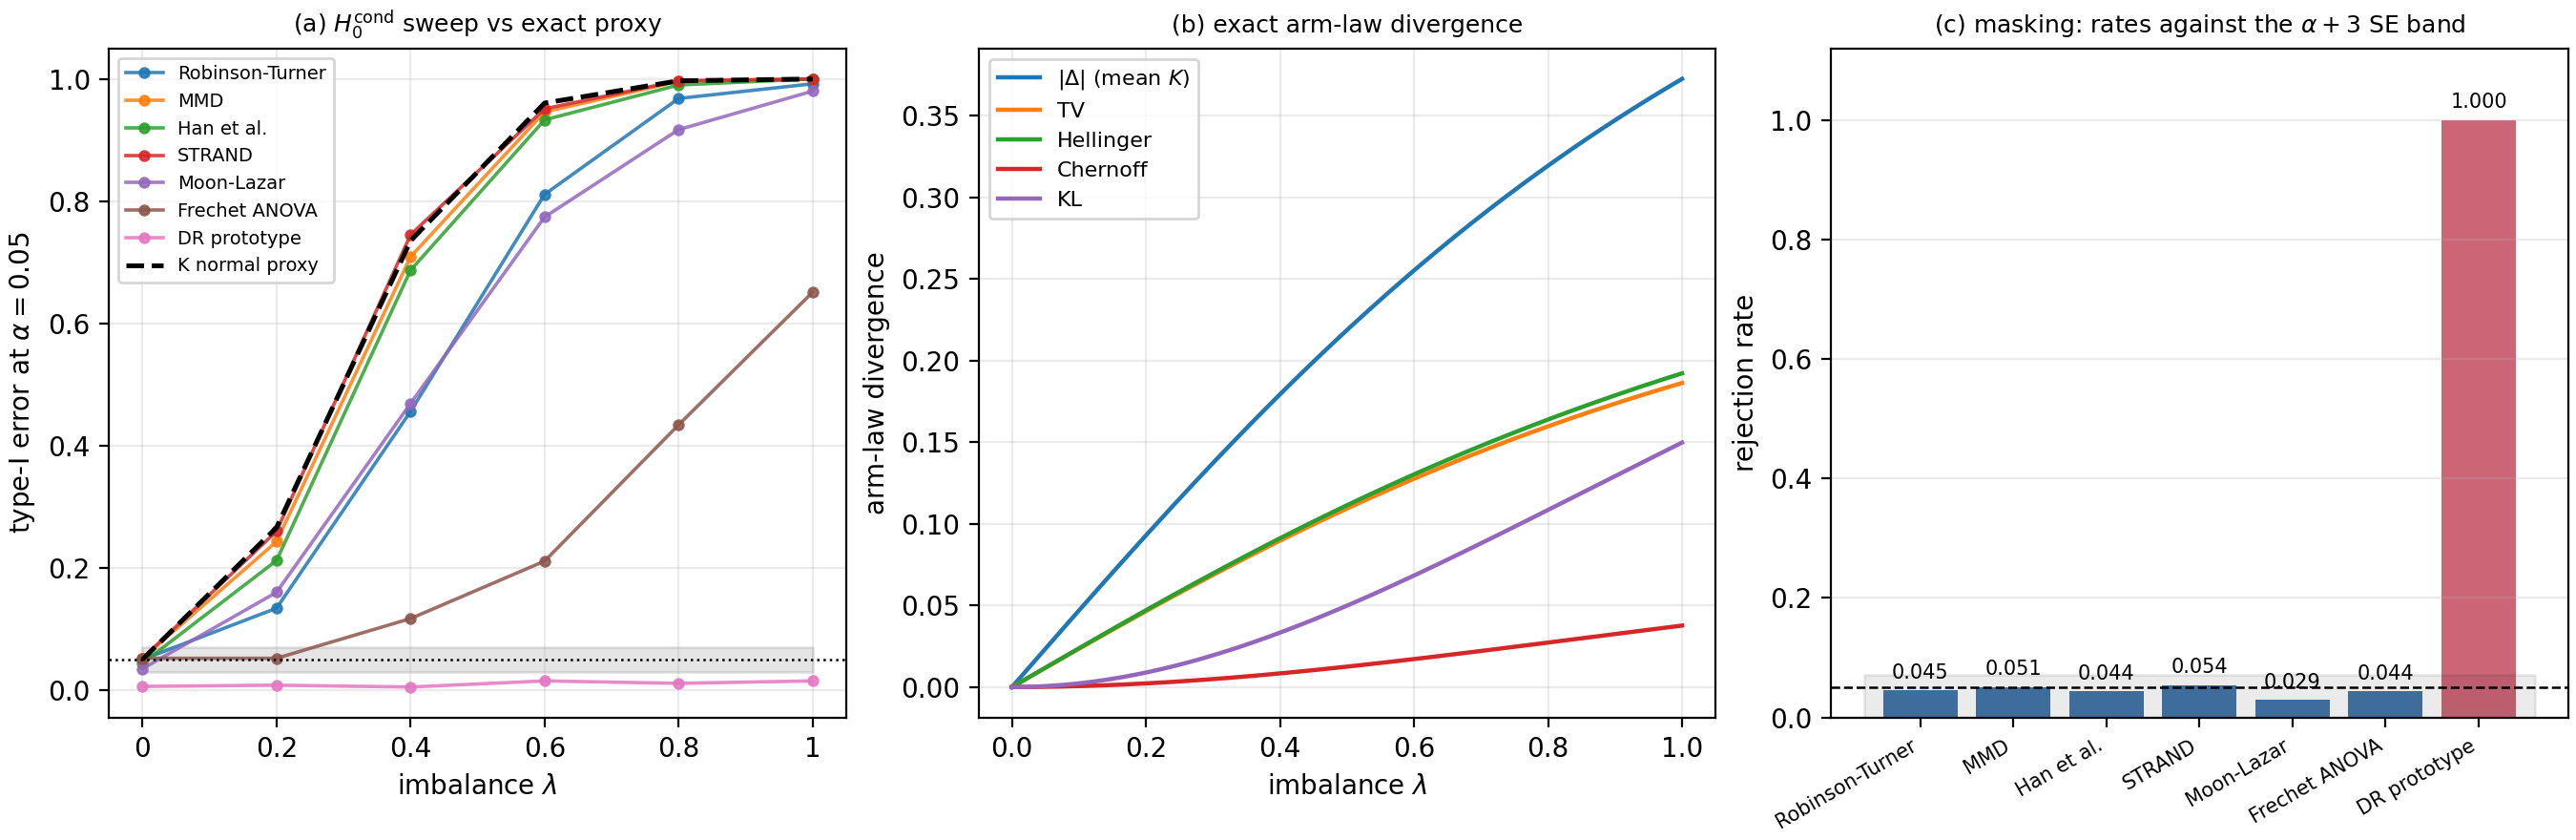
\includegraphics[width=\textwidth]{appendix_c1_masking_mechanism.png}
\caption{Recorded leakage and masking mechanisms. The panels show the conditional-law sweep under the causal null, the exact arm-law divergences, and the masking rates, with the exact mechanism proxy overlaid. The sweep and masking panels concern $H_0^{\mathrm{cond}}$ for the unadjusted columns and $H_0^{\mathrm{out}}$ for the adjusted column; replication counts and Monte Carlo standard errors are given in the text.}
\label{fig:app-masking}
\end{figure}

\subsubsection{Local limit under Pitman shifts and the drift identity}
\label{app:local}

Assumptions: (B1) repeated clouds, location-shift array, uniformly bounded second moments; (B2) causal consistency and arm-specific exchangeability; (B3) positivity $\kappa\le e(x)\le1-\kappa$, maintained for the true and fitted propensity; (B4) a correct finite-basis span with parametric regression rate, an $L^2$-consistent propensity, the product rate, and a possibly nonzero direction residual $r_g=g-P_Mg$; (B5) entropy and Donsker conditions; (B6) fixed-fold cross-fitting; (B7) shared Gaussian multipliers with moment and variance conditions; (B8) a fixed nonzero direction with a well-defined standardized drift $h$. A correction to (B3) is part of the statement: the implementation clips only exact $0$ and $1$, interior fitted propensities can fall below $10^{-2}$, and $\kappa$ is a maintained assumption, not an enforced floor; the strongly confounded prognostic design has $\E[e^{-2}]=\infty$, so (B3) is not verified there.

The exact pointwise shift identity is false as stated: for a treated unit the score difference is $n^{-1/2}g_d(t)(1-A/e(X))$, not $n^{-1/2}g_d(t)$, and a direct calculation exhibits the failure for any $e\in(0,1)$. What is true and used is the exact mean identity $\E_{P_n}[\varphi_d(t,\cdot;\eta_0)]=\E_{P_n}[\varphi_d(t,\cdot;\eta_n)]=\psi_{d,n}(t)$; the regular limit survives with an added $O_P(n^{-1/2})$ empirical-process term replacing the invalid cancellation. Under (B1) to (B8) with $h\equiv0$, $\sqrt n(\hat\psi_d-\psi_{d,n})\Rightarrow G$ in $\ell^\infty(T)^D$ with the oracle efficient-influence covariance, and $T_n^{\mathrm{out}}\Rightarrow\max_d\sup_t\abs{G_d(t)+g_d(t)}$. Completeness is modulo gap G1 (cross-fitting linearization, cited from \cite{chernozhukov_dml_2018,new_robins_2018}), gap G2 (uniformity of the triangular Donsker condition, assumed), and gap G3 (multiplier quantile under the local sequence, cited from \cite{cck_2013} and adapted by contiguity). The local power is $\pi(g)=\Prob(\max_d\sup_t\abs{G_d(t)+g_d(t)}>c_{1-\alpha})$ with $\pi(0)=\alpha$ and strict power for nonzero directions with non-degenerate restricted covariance. The strictness step invokes \cite{anderson_1955,perlman_1988}; it is asserted rather than fully proved for the infinite-dimensional case, with no counterexample found. The detection boundary is the $n^{-1/2}$ scale with marginal constant $\tau\approx\sigma_0(c_{1-\alpha}+z_\beta)/\abs{h}$. The non-central branch $G+g+h$ is an adaptation; the explicit drift formulas carry a missing $\sqrt n$ factor and a sign correction and are not restated as proved.

The exact drift identity is: with $u_i=1-e_i/\hat e_i$, $w_i=1-(1-e_i)/(1-\hat e_i)$, regression error $e_{a,i}$, and residual $r_{a,d}$,
\[
\E[\hat\varphi_i(t)\mid X_i,\hat\eta]=\mu^{(n)}_{1,i}-\mu_{0,i}-u_i\big(r_{1,d}(t,X_i)+n^{-1/2}r_{g,d}(t)\big)+w_ir_{0,d}(t,X_i)+u_ie_{1,i}(t)-w_ie_{0,i}(t),
\]
so $\sqrt n(\hat\psi_d-\psi_{d,n})=G_n\varphi_d(\cdot;\eta_0)+\mathrm{amp}_nr_{g,d}+R_n$ with $\mathrm{amp}_n=n^{-1}\sum_i(e(X_i)/\hat e_i-1)=-n^{-1}\sum_iu_i$ and conditionally centred $R_n$; the drift is $O_P(\delta_n)$, $\delta_n=\norm{1-e/\hat e}$, not $n^{-1/2}$. Under the fitted nuisances the effective shift is $g_{\mathrm{eff},n}=g+\kappa_n(g-P_Kg)$ with $\kappa_n=\E[e/\hat e_n]-1$. This is a finite-$n$ expansion, not a local limit: a consistent propensity gives $\kappa_n\to0$ and the correction vanishes. An asymptotic version would need a mean-ratio consistency rate for the propensity learner; that rate is neither assumed by \cite{kim_lee_tce_2026} nor proved here, and the exact finite-sample statement is the drift classification $\mathrm{amp}_nr_g=O_P(\delta_n)$. Under randomisation with $e=1/2$, $\kappa_n\ge0$ is proved by Jensen.

The projection residuals are $1.1\times10^{-16}$ (mean), $0.1413$ (bump), $0.7130$ (frequency). The paired drift identity holds at machine precision in the $t$ average and within $0.58$ MC SE at the worst grid point. For the frequency cell under the strongly confounded prognostic design at $n=500$, the pre-registered screen is false: empirical $0.730$ against naive $0.628$, gap $+0.102$ (MC SE $0.026$). The corrected point prediction is $0.783$, gap $-0.053$; under common random numbers about $-0.041$, with the $\kappa_n\pm1$ SE band $[-0.071,-0.034]$ crossing the $0.06$ tolerance at one standard error. Raising the outcome basis from five to seven functions removes the out-of-span fraction and returns the projection to its oracle value ($5.0103$ against $4.9930$); the pre-registered basis comparison is underpowered (gap $+0.0624$, MC SE $0.068$), so the projection certificate is the mechanism evidence. The correction resolves only the $n=500$ DR Gaussian-shift comparison at a post-hoc corrected point prediction. The pre-registered screen and the full-fleet validation remain false for the uncorrected prediction ($51$ scored rows, $9$ over tolerance, $17$ beyond two standard errors); the bump direction is inside noise and not claimed; the completed exact-design record shows DR below the unadjusted test at $n=200$ and $n=500$ in every direction (mean gaps $0.14$ to $0.19$), so asymptotic equality is not translated into finite-$n$ power equality.

\begin{figure}[t]
\centering
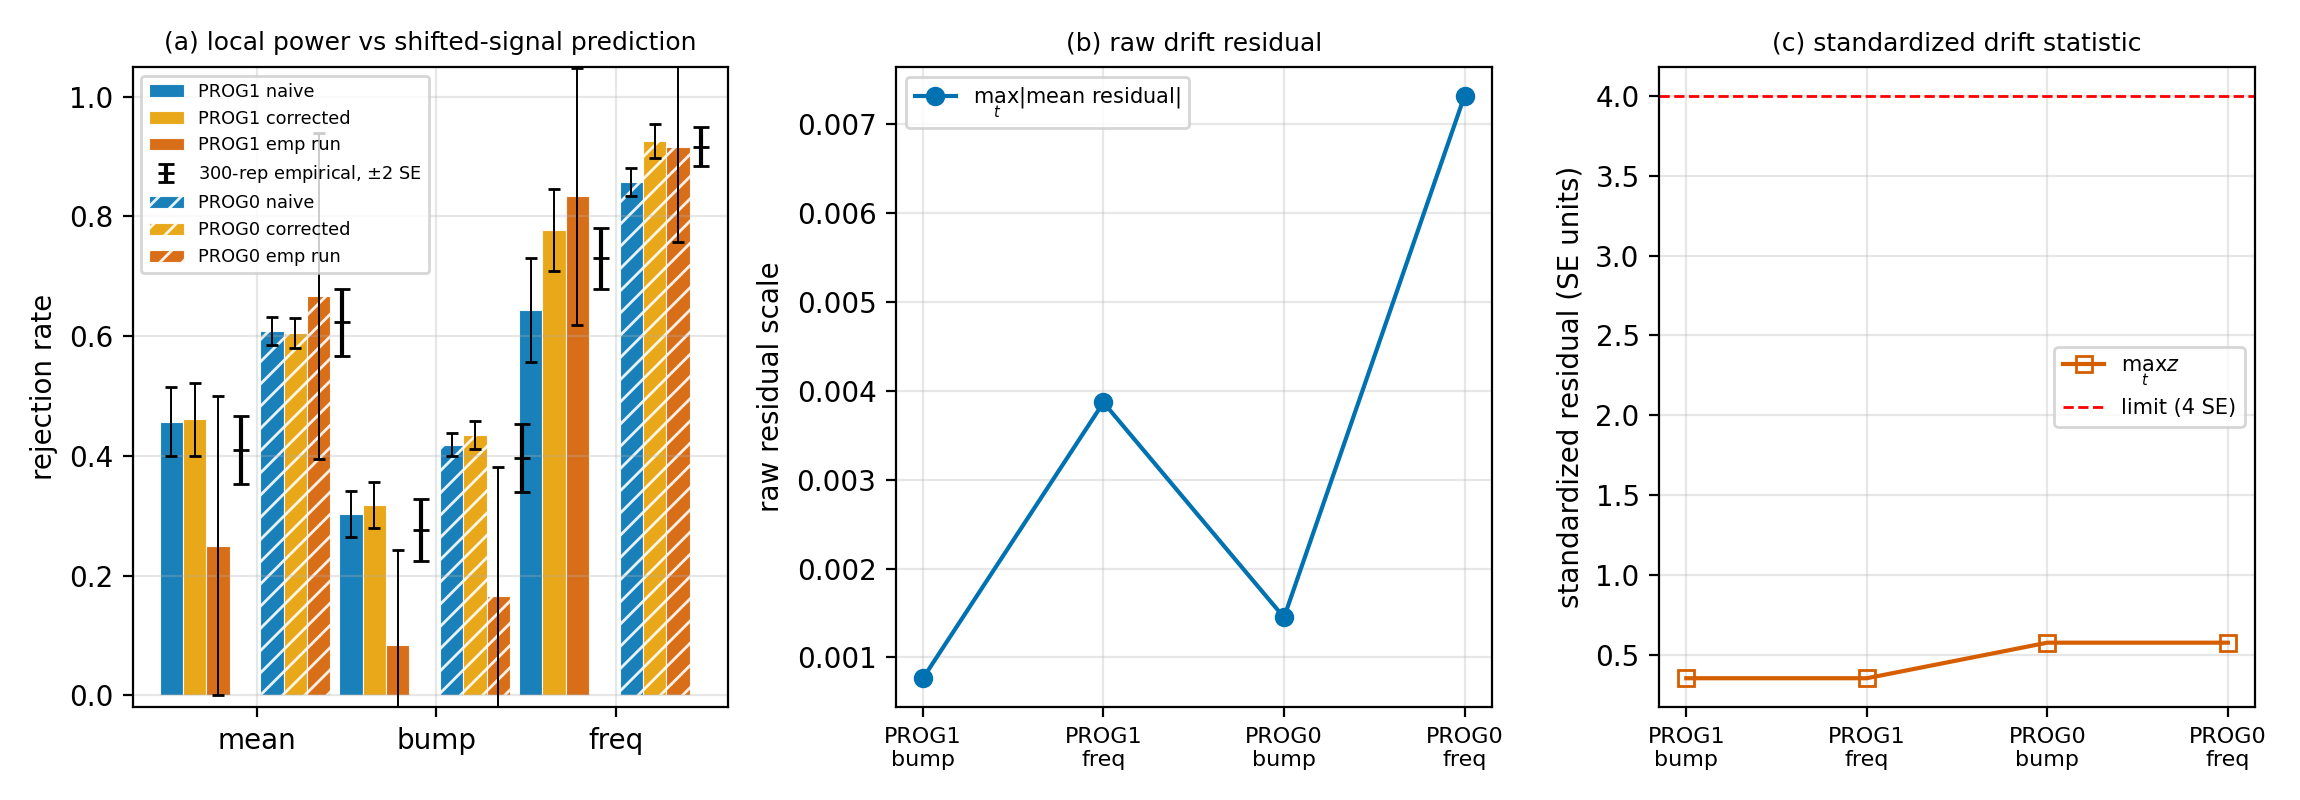
\includegraphics[width=\textwidth]{appendix_t3_local_limit.png}
\caption{Local limit at reduced replication count: local-power bars against the shifted-signal prediction, the $300$-replication empirical overlay, the raw drift residual, and the standardized drift statistic (limit four standard errors). Setting codes denote the nuisance design and assignment regime: PROG0 and PROG1 are prognostic outcomes under randomised and confounded assignment respectively, and NONPROG0 and NONPROG1 are the X-independent-outcome analogues. Null tested: $H_0^{\mathrm{out}}$; bars are two Monte Carlo standard errors where the cell has $12$ replications.}
\label{fig:app-t3-local}
\end{figure}

\begin{figure}[t]
\centering
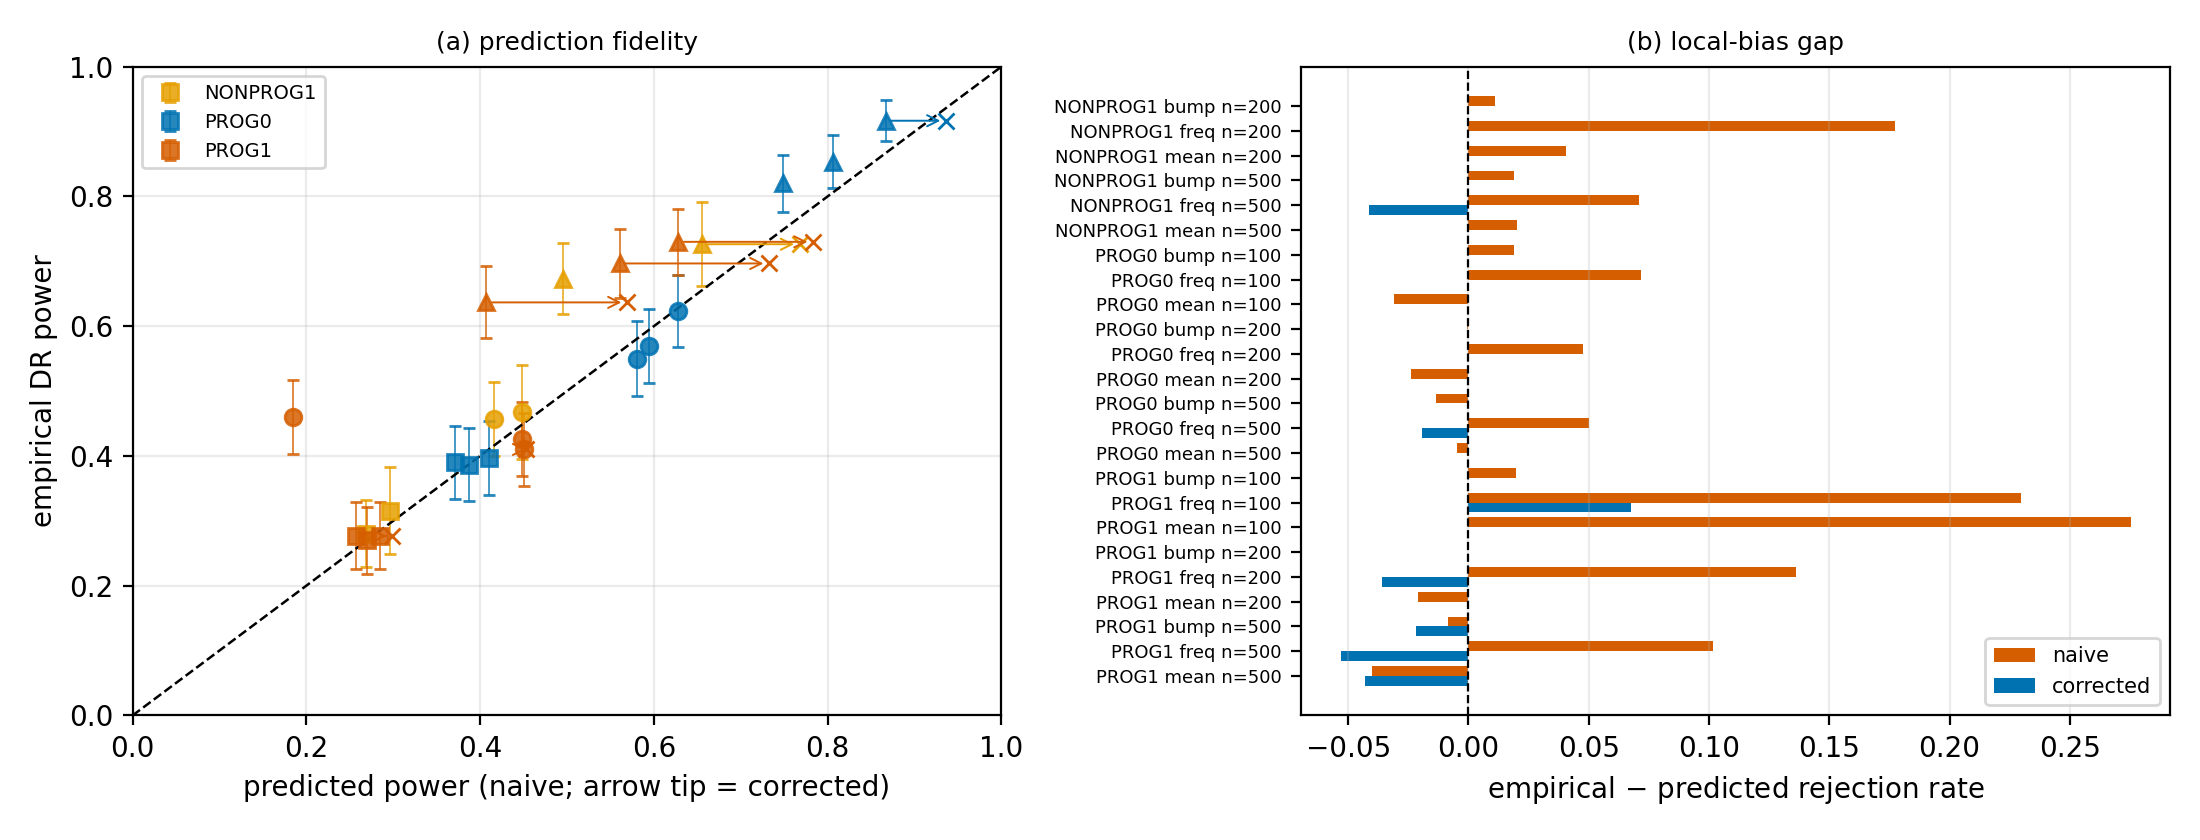
\includegraphics[width=\textwidth]{appendix_t7_mismatch.png}
\caption{The finite-sample mismatch and its correction: predicted versus empirical power before and after the truncation correction, and the per-cell local-bias gap. Setting codes follow Figure~\ref{fig:app-t3-local}. Null tested: $H_0^{\mathrm{out}}$. The correction is a finite-$n$ expansion, and the mean-ratio rate it uses is not proved.}
\label{fig:app-t7-mismatch}
\end{figure}

\begin{figure}[t]
\centering
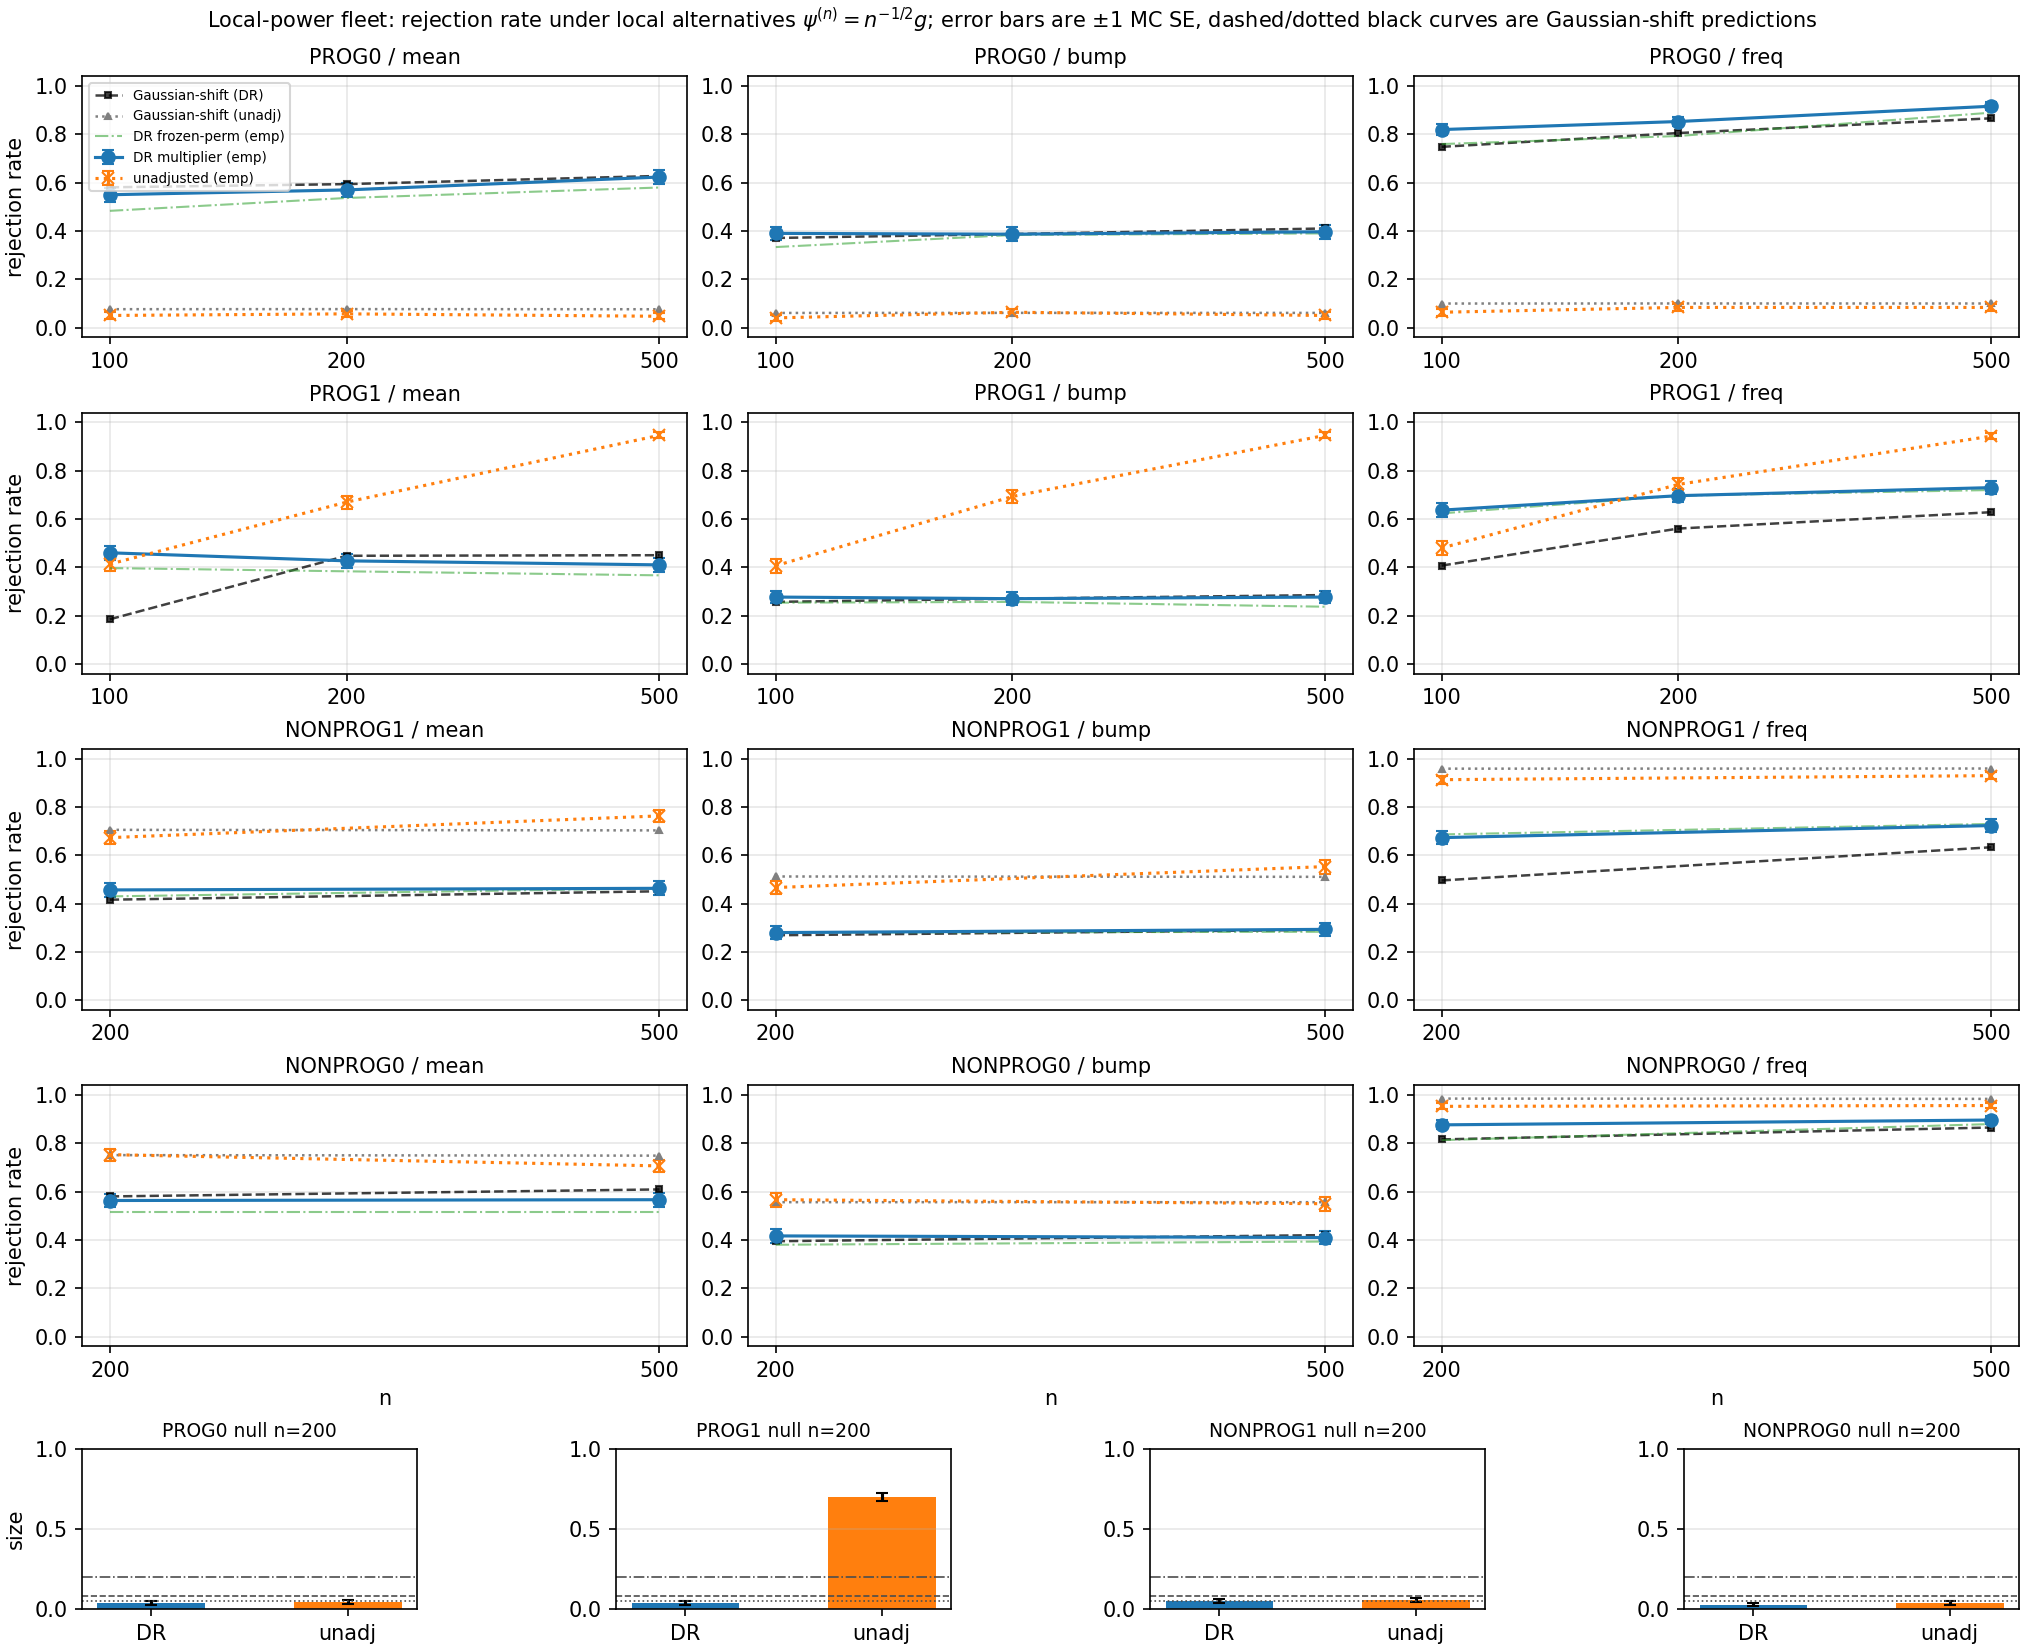
\includegraphics[width=\textwidth]{appendix_t10_full_fleet.png}
\caption{The complete local-power fleet across settings, directions, and sample sizes, with Monte Carlo standard errors and Gaussian-shift predictions, including the null-size panels. Setting codes follow Figure~\ref{fig:app-t3-local}. Null tested: $H_0^{\mathrm{out}}$ for the adjusted statistic and the corresponding unadjusted null for the baseline; the pre-registered screen remains false for the uncorrected prediction.}
\label{fig:app-local-fleet}
\end{figure}

\subsubsection{Semiparametric bound, attainment, and the minimax boundary}
\label{app:efficiency}

Assumptions: (E1) independent clouds; (E2) causal consistency and arm-specific exchangeability; (E3) strict positivity and eventual fitted positivity; (E4) finite second moments of $\norm{Z}$; (E5) a locally nonparametric model; (E6) for attainment, fixed-fold cross-fitting with $L^2$ consistency, the product rate, and eventual positivity. The $Z$-reduction shows the rest of the cloud is ancillary for the summary functional. Under (E1) to (E5), the score $\varphi_d(t,O;\eta)$ displayed in the main text is the efficient influence function of $\psi_d(t)$, with variance $\mathrm{Var}(\tau_d(t,X))+\E[\mathrm{Var}(Z_d(t)\mid X,A=1)/e(X)]+\E[\mathrm{Var}(Z_d(t)\mid X,A=0)/(1-e(X))]$ and the analogous covariance kernel. A known propensity leaves the bound unchanged \cite{hahn_1998,hirano_imbens_ridder_2003}. On a fixed grid the bound is the projected matrix, the coarsened-observation submodel costs no efficiency, and the bound does not depend on $q$ beyond the retained coordinates. Cross-fitted AIPW attains the bound at fixed $q$ under the product rate, via a mean-zero leading process, a cross-fitted empirical-process term, and a von Mises remainder bounded by $\kappa^{-1}\norm{\hat e-e}_{L^2}(\norm{\hat m_1-m_1}_{L^2}+\norm{\hat m_0-m_0}_{L^2})=o_P(n^{-1/2})$. Functional attainment is an adaptation with the uniform-in-nuisance equicontinuity gap declared; the infinite-dimensional operator bound is cited and adapted, and its convolution theorem was not verified end to end. Scope: fixed $q$; no increasing or data-dependent grid; no efficiency of the sup-norm or max-$t$ procedure; no finite-sample efficiency.

Numerically, the oracle identity, propensity orthogonality, and same-sample parametric criterion pass. Four of seven pre-registered criteria fail: cross-fitted ratio $+0.1502$ at $n=1000$ and $+0.0334$ at $n=4000$; known-versus-estimated spread $0.1124$; subgrid projection inheriting the inflation; coordinate-averaged overfit bias $+0.0289$ against a $3$-SE bound of $0.0507$ (the per-coordinate bias changes sign). All four are consistent with the asymptotic statement and locate a finite-$n$ propensity variance inflation of roughly $90$ to $100$ over $n$ in the surrogate design, not derived and not extrapolated; this channel must not be added to the mean-ratio drift of Section~\ref{app:local}.

\begin{figure}[t]
\centering
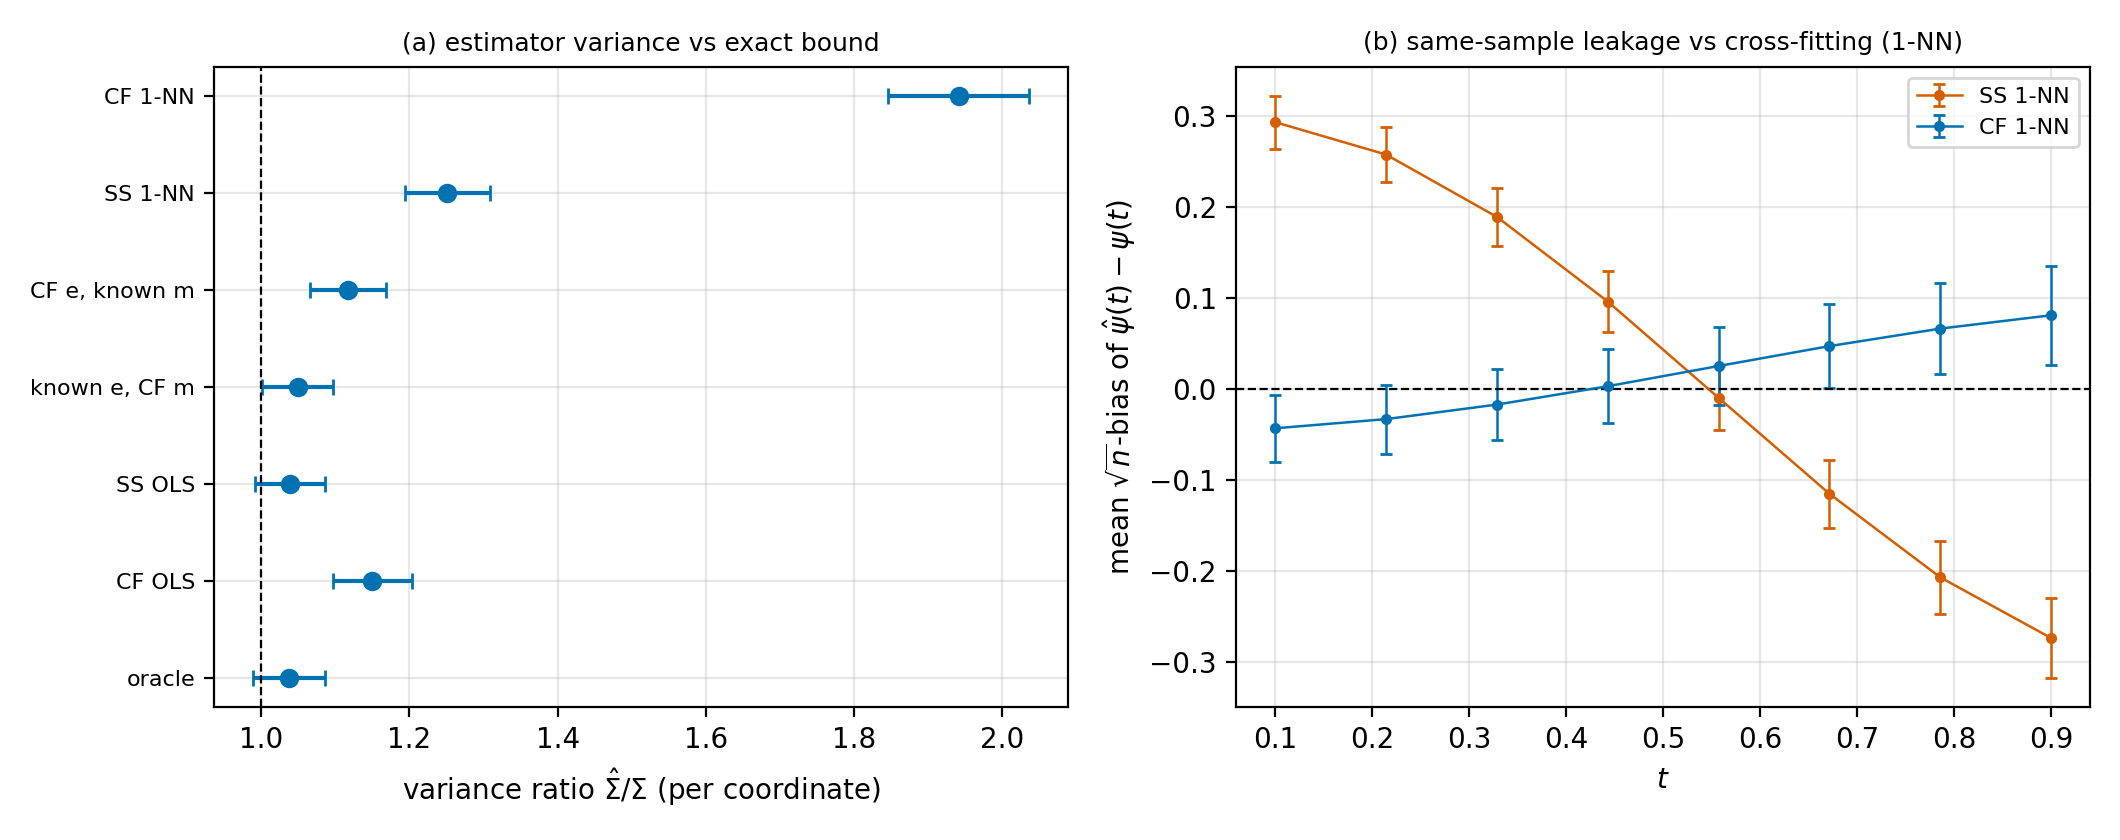
\includegraphics[width=\textwidth]{appendix_t4_efficiency.png}
\caption{Efficiency checks: per-coordinate variance ratios against the exact bound with two Monte Carlo standard errors, and the same-sample versus cross-fitted $1$-nearest-neighbour bias paths. Null tested: $H_0^{\mathrm{out}}$ at fixed grid dimension. Four of seven pre-registered criteria miss, so no finite-sample efficiency is claimed.}
\label{fig:app-t4-eff}
\end{figure}

\subsubsection{Minimax boundary and regime comparison}
\label{app:minimax}

The lower bound is proved on a Gaussian submodel: $q$ fixed, $A_i\sim\mathrm{Bern}(1/2)$ independent of $X_i$ and the outcomes, $Z_i\mid A_i=a\sim N(\mu_a,\sigma^2I_q)$, $\mu_0=-\psi/2$, $\mu_1=\psi/2$. The sufficient statistic $S=\sum_i(2A_i-1)Z_i$ has the assignment-invariant law $N(n\psi/2,n\sigma^2I_q)$; the log-likelihood ratio is a Gaussian shift with $z=n\norm{\psi}^2/(4\sigma^2)$. Le Cam's two-point method \cite{le_cam_1986} with the chi-square identity gives: any test of level at most $\alpha$ and type-II error at most $\beta$ needs L2 separation at least $2\sigma\sqrt{L_{\alpha,\beta}/n}$, $L_{\alpha,\beta}=\log(1+4(1-\alpha-\beta)^2)$, equal to $2.1713\,\sigma n^{-1/2}$ at $\alpha=0.05$, $\beta=0.20$. The constant is not claimed sharp. The smooth-class adaptation gives the classical exponent $n^{-2\beta/(4\beta+1)}$, numerically slope $-0.4147$ against $-0.4$; no self-contained Fano or Assouad proof is supplied. Replacing $\lambda_{\max}(\Sigma)$ by $\lambda_{\max}(\Sigma_{\mathrm{DR}})$ is a \emph{conjecture}; the sharp semiparametric minimax constant is not claimed. At randomisation the baseline is target-matched with $\Sigma_{\mathrm{base}}-\Sigma_{\mathrm{DR}}=\mathrm{Cov}(m_1+m_0)\succeq0$, giving $\mathrm{ARE}(\mathrm{DR}:\mathrm{base})=1.1125$ (prognostic) and $1.0000$ (non-prognostic); under confounding its limit is $1.0590$ against $\psi=0$ and it is invalid for $H_0^{\mathrm{out}}$. No dominance over \cite{han_kim_kim_2026} is claimed: their null is strictly stronger at randomisation and their bounded-density condition is not verified on the harness.

\begin{figure}[t]
\centering
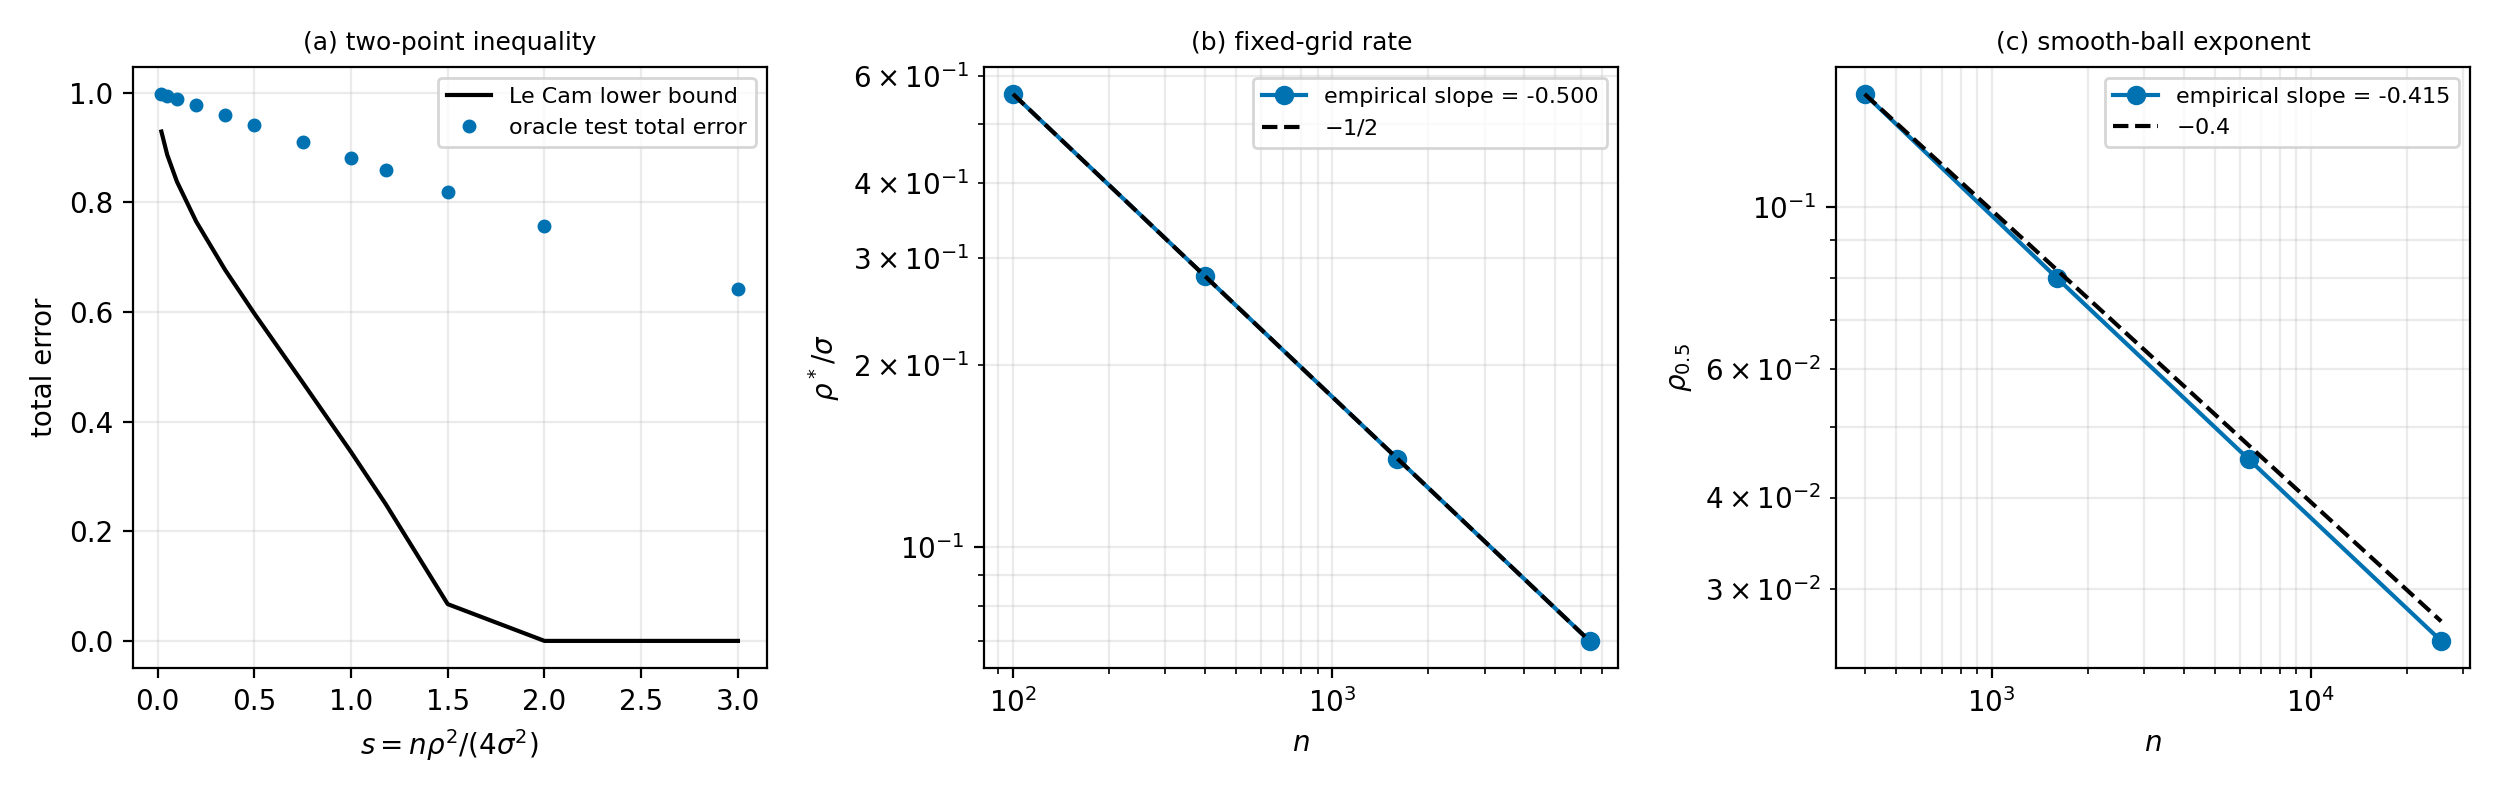
\includegraphics[width=\textwidth]{appendix_t8_minimax.png}
\caption{Minimax checks: the two-point inequality against the Le Cam bound, the fixed-grid rate with the $-1/2$ reference slope, and the smooth-ball exponent. Null tested: $H_0^{\mathrm{out}}$. The sharp minimax constant remains a conjecture; only the bound and the rate slope are proved.}
\label{fig:app-t8-minimax}
\end{figure}

\subsubsection{ARE among target-matched tests}
\label{app:are}

Assumptions: A1 identification with strict positivity and finite second moments; A2 nuisance limits with the cross-fitted remainder $o_P(n^{-1/2})$ under the product rate; A3 fixed-fold cross-fitting; A4 the local limit and calibration imported from Section~\ref{app:local} with its three gaps. The exact algebra gives $\mathrm{Var}(S_D)=\mathrm{Var}(w'(m_1-m_0))+\E[w'\sigma_1w/e_0+w'\sigma_0w/(1-e_0)]$ and
\[
\mathrm{Var}(S_I)-\mathrm{Var}(S_D)=\E\Big[\big(\sqrt{(1-e_0)/e_0}\,w'm_1+\sqrt{e_0/(1-e_0)}\,w'm_0\big)^2\Big]\ge0 .
\]
In the empty cocoon ($e_0=1/2$, $m_1=m_0=c$ a.s.) the DR score, estimated-propensity IPW, correctly specified arm-constant outcome regression, and unadjusted contrast share the influence function $2(2A-1)w'(Z-c)$, so the ARE is one among them; the known-propensity IPW score is the exception. Outside the location-shift cocoon the unadjusted and Robinson-Turner tests target a different null and no superiority over them may be claimed. For $\lambda>0$ the covariance order $\mathrm{Cov}(S_I)\succeq\mathrm{Cov}(S_D)$ holds with the displayed gap; misspecified IPW or outcome-regression procedures are size-broken and excluded from the class, so no size-adjusted power comparison exists for them and the earlier size-adjusted dominance reading is withdrawn. The frozen stratified permutation is valid only in the exchangeability regime; outside it the permutation law centres at the observational contrast and the test is not level-$\alpha$ (recorded weak-null rates $0.20$ to $0.25$; a confounded bake-off reading $0.36$ against $0.76$). The studentized max-$t$ power monotonicity under the Loewner order is a \emph{conjecture}, supported in $200$ of $200$ random probe configurations. The small-$n$ counterexample is part of the record: at $n=50$ under randomisation the DR multiplier rejects the mean shift at $0.110$ against $0.800$ for Robinson-Turner and $1.000$ for the other unadjusted tests; the surrogate variance ratio is $1.344$ and the calibrated power drop $0.0590\pm0.0095$.

\begin{figure}[t]
\centering
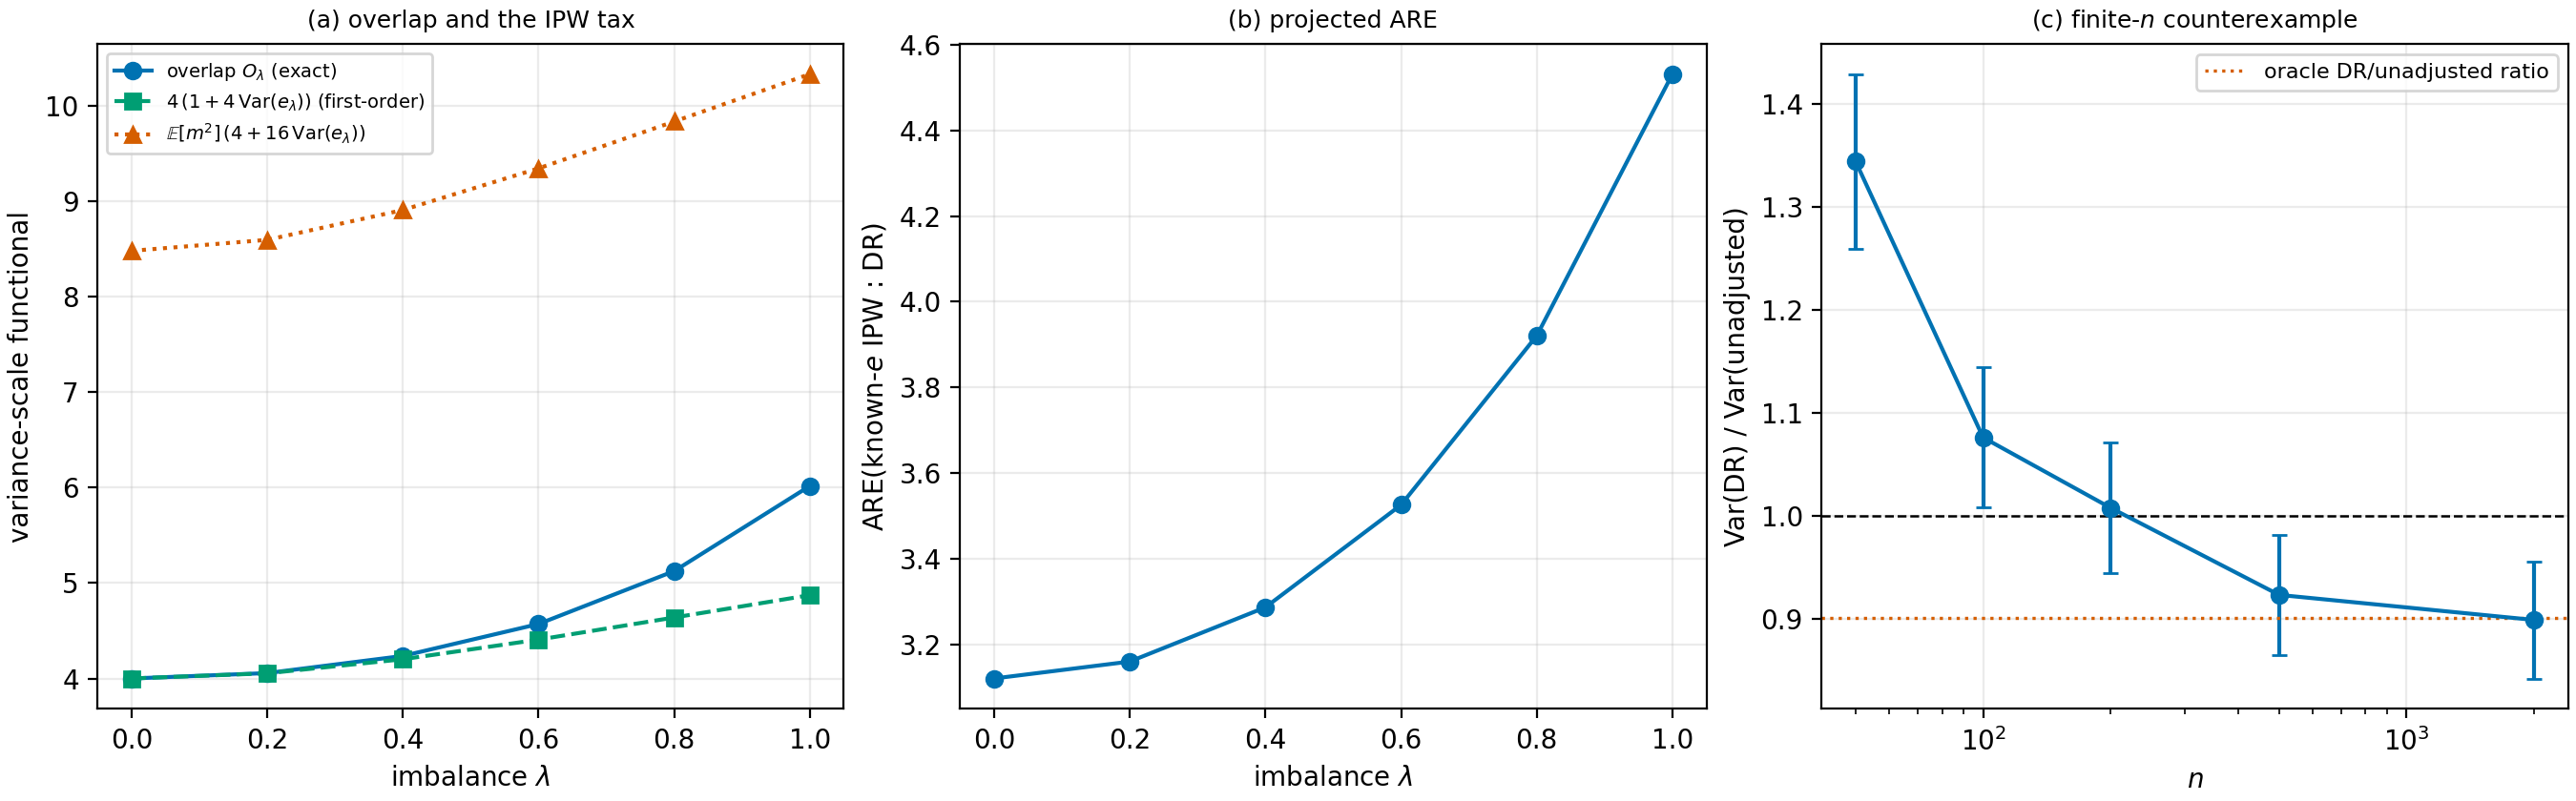
\includegraphics[width=\textwidth]{appendix_t5_are.png}
\caption{Target-matched relative efficiency: overlap, the first-order inverse-probability tax, the exact lower bound, the projected efficiency ratio, and the finite-sample variance-ratio counterexample. Null tested: $H_0^{\mathrm{out}}$ within the target-matched class of Definition~\ref{def:class}; max-$t$ power monotonicity remains a conjecture.}
\label{fig:app-t5-are}
\end{figure}

\subsubsection{Fixed-grid max-\texorpdfstring{$t$}{t} validity and local power}
\label{app:distgrid}

Assumptions: (D1) identification for the finite-grid vector; (D2) positivity; (D3) bounded features and scores; (D4) fixed folds with double machine learning nuisance rates, parametric for the frozen learners; (D5) a fixed active set with uniformly positive score variances and an eventually correct sample active set; (D6) Gaussian multipliers independent of the data. The local and growing-grid results add (D4-u) uniform DML along the local sequence and (D5-u) uniform separation; both remain assumptions. Under (D1) to (D6) the cross-fitted linearization is an adaptation with untracked constant, studentisation costs $O_P(\log(qn)/\sqrt n)$, and the Gaussian and multiplier approximations of \cite{cck_2013} apply to the active subvector with $\log(qn)$ substituting conservatively for $\log(\abs{J}n)$. The size error is of order $B\,n^{-1/8}\log^{7/8}(n)$ up to untracked constants, and the frozen-learner remainder is dominated at the parametric rate. Uniformity over the nominal level holds; uniform-in-$n$ validity is not claimed and the $n=200$ confounded cell is the counterexample. A growing grid remains valid under $\log(q_nn)=o(n^{1/7})$, with the sharper modern bound weakening this to $o(n^{1/5})$; only the conservative form is cited.

Along $\delta^{(n)}=n^{-1/2}h$, the studentized statistic converges to $\max_{j\in J}\abs{Z_j+h_j/\sigma_j}$, $Z\sim N(0,R)$, so the power function is explicit and the boundary lies at the $n^{-1/2}$ scale. That this scale is also a lower bound for arbitrary tests is not proved here; only the fixed-grid Le Cam bound of Section~\ref{app:minimax} is available. The null critical value grows with the active multiplicity, bounded above by the union bound and below by the single-coordinate quantile. Finite-grid control certifies only the projected expected measure: the projection has a non-trivial kernel, witnessed by two one-atom diagrams with identical projected vectors and distinct measures (unnormalised total variation $0.093312$), against which the test has asymptotic power $\alpha$. In the strong-confounding decomposition the oracle score law has excess kurtosis $+0.56$; at $n=200$ the oracle arm rejects at $0.070$ and the estimated arm at $0.096$ (paired gap $+0.026$, SE $0.007$), and both are in band at $n=500$ ($0.058$ and $0.066$). The pre-registered mechanism rule returns neither hypothesis and the grid-size sanity criterion fails as recorded; fitted restoring sizes are $173$ to $369$, all below $500$. No positivity failure is claimed (operative margin $1/4$) and no rate-condition violation is claimed; the binding channel is the finite-$n$ multiplier approximation with estimated scores.

\begin{figure}[t]
\centering
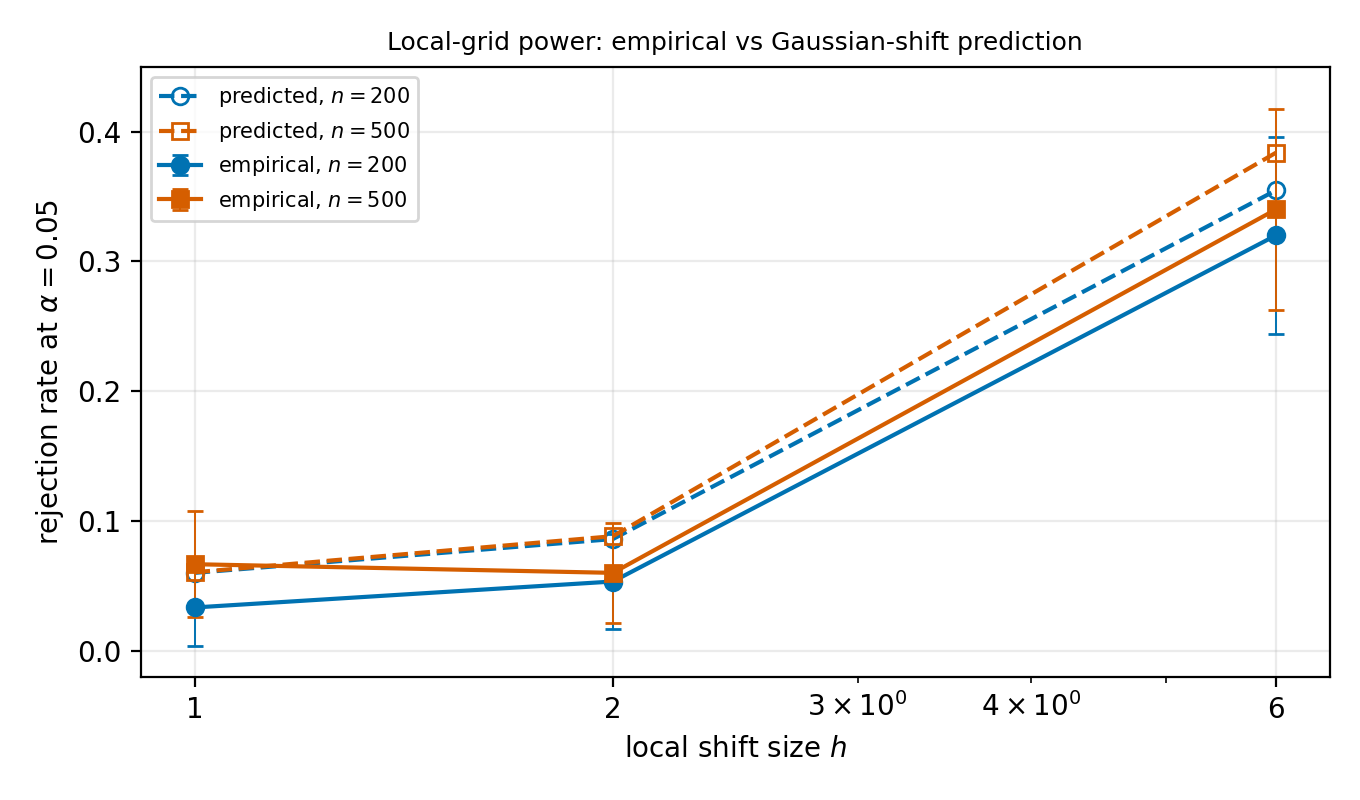
\includegraphics[width=\textwidth]{appendix_t6_distgrid_local.png}
\caption{Fixed-grid local power at $n=200$ and $n=500$, empirical versus Gaussian-shift prediction. Null tested: $H_0^{\mathrm{dist,grid}}$; the target is the projection onto the frozen grid, not the unprojected expected measure.}
\label{fig:app-t6-distgrid}
\end{figure}

\begin{figure}[t]
\centering
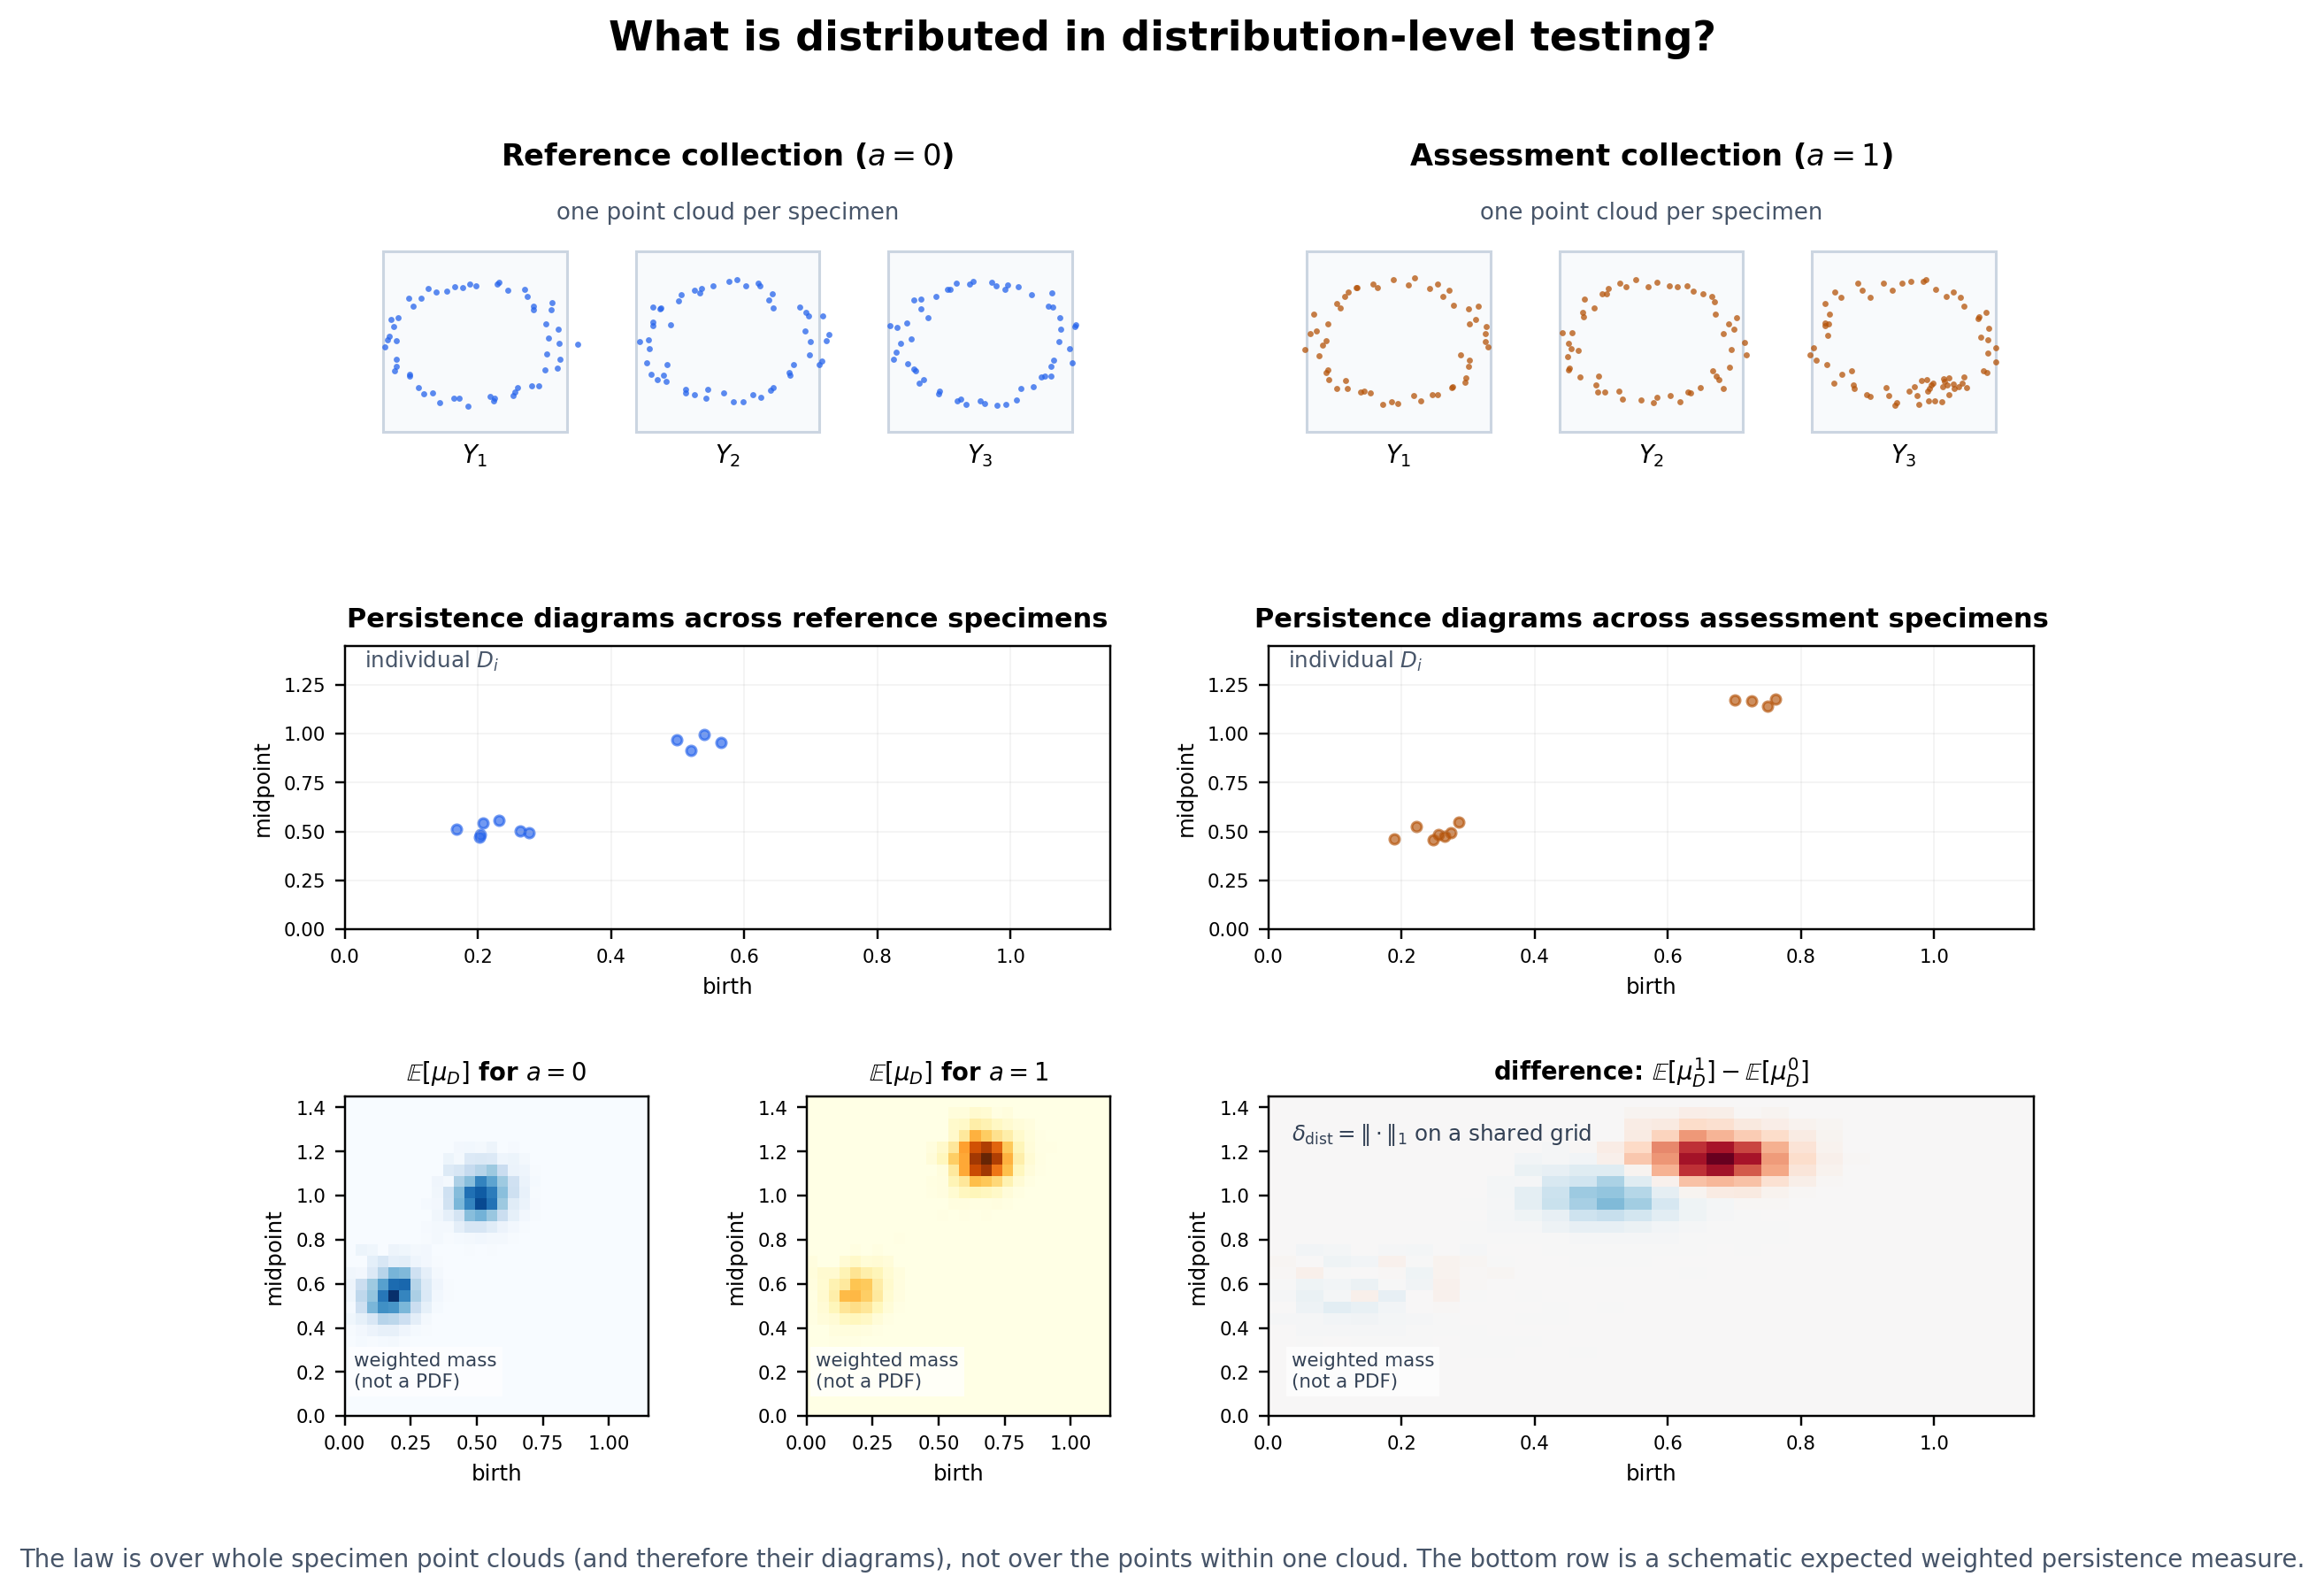
\includegraphics[width=\textwidth]{appendix_distribution_explainer.png}
\caption{Schematic of the distribution-level target: one point cloud per unit, its persistence diagram, and the expected weighted persistence measure on the frozen grid. The figure is a schematic and carries no empirical result.}
\label{fig:app-explainer}
\end{figure}

\subsubsection{Multiplicity FWER}
\label{app:multiplicity}

Assumptions: (A1) independent units with fixed finite degree and grid sets; (A2) the outcome null; (A3) cross-fitted linearization with $2+\delta$ moments, the cross-fitting extension labelled as an adaptation; (A4) the moment and variance conditions of \cite{cck_2013}; (A5) estimated-score consistency in mean square; (A6) a continuous strictly increasing maximum cdf at the quantile and integer $\alpha(B+1)$; (A7) the joint per-degree coupling for the studentized comparator, stated rather than derived. The proof reduces the studentized statistic to the oracle maximum, applies the Gaussian and multiplier approximations to the shared-multiplier construction, replaces estimated scores at $o_P(1)$, and closes by rank monotonicity: the conditional rejection function is nonincreasing, so
\[
\Prob(p_n^{\mathrm{unstud}}\le\alpha)\le\frac{\lfloor\alpha(B+1)\rfloor}{B+1}+\varepsilon_n\le\alpha+\varepsilon_n .
\]
The pooled-studentized comparator is exactly symmetric in the $B+1$ augmented values and exactly scale invariant; under (A7) its level is at most $\alpha$, and the source convention is only asymptotically valid as $B$ grows. The unstudentized maximum collapses to its null level when a null degree's scale diverges while the studentized decision is exactly constant; the recorded fleet realizes the contrast ($0.7025\to0.0525$ against $0.7142\to0.7092$). The frozen permutation is finite-sample exact only in the exchangeability regime, and outside it the confounded weak-null rates are $0.198$ to $0.248$. The one recorded miss is reported strictly: shared rate $0.0364$ (MC SE $0.0037$), $3.63$ standard errors below $\alpha$, with seed-stability pooled rate $0.0312$ (SE $0.0017$, zero of four seeds in band) against Gaussian $0.0465$ (SE $0.0021$, four of four). This falsifies finite-sample equality of size, not upper control. No finite-sample exactness, no literal continuum-sup result, and no general stochastic-order statement is claimed; the dependence-preservation order remains a \emph{conjecture}.

\begin{figure}[t]
\centering
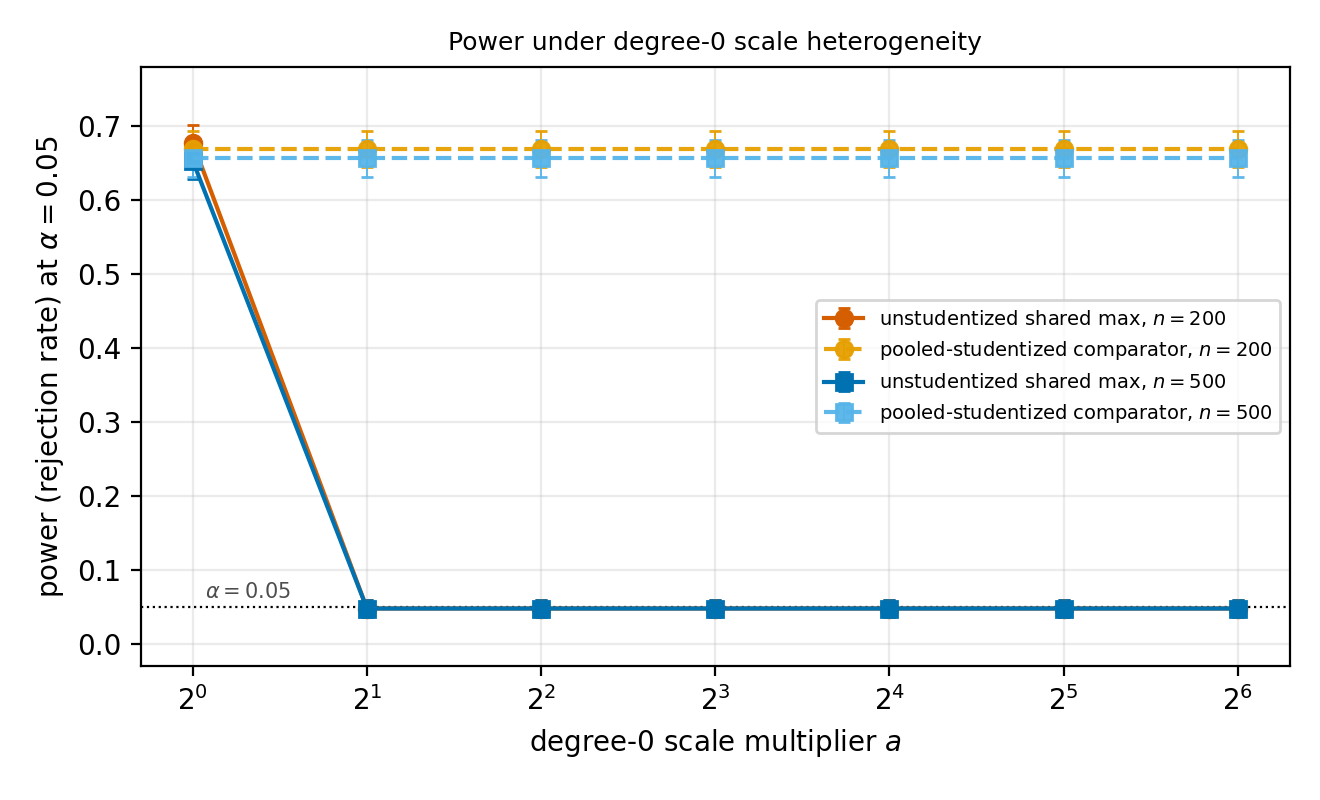
\includegraphics[width=\textwidth]{appendix_t9_multiplicity.png}
\caption{Power versus degree-$0$ scale heterogeneity for the unstudentized shared maximum and the pooled-studentized comparator. Null tested: $H_0^{\mathrm{out}}$ over the degree family; the studentized decision is exactly scale invariant, while the unstudentized maximum collapses when one degree's scale dominates.}
\label{fig:app-t9-mult}
\end{figure}

\subsection{Oracle fleet detail}
\label{app:oracle}

Table~\ref{tab:app-oracle} prints all $24$ cells of the oracle calibration fleet ($500$ replications per cell, MC SE $0.0071$ to $0.0109$). Null tested: $H_0^{\mathrm{out}}$; the alternative is the fixed oracle shift. Alternative rates are $0.990$ to $1.000$ (multiplier) and $0.944$ to $1.000$ (permutation). Two null cells at $0.026$ sit below the pre-registered $0.03$ edge (multiplier at $n=500$, $\lambda=1.0$; permutation at $n=200$, $\lambda=0.5$) and remain open calibration items; no band was retuned.

\begin{table}[t]
\centering
\small
\setlength{\tabcolsep}{5pt}
\begin{tabular}{@{}rrcccc@{}}
\hline
$n$ & $\lambda$ & null mult. & null perm. & alt. mult. & alt. perm. \\
\hline
50 & 0.0 & 0.064 & 0.040 & 0.992 & 0.972 \\
50 & 0.5 & 0.042 & 0.034 & 0.996 & 0.970 \\
50 & 1.0 & 0.044 & 0.046 & 0.990 & 0.944 \\
100 & 0.0 & 0.056 & 0.038 & 1.000 & 0.994 \\
100 & 0.5 & 0.056 & 0.034 & 1.000 & 0.994 \\
100 & 1.0 & 0.048 & 0.052 & 1.000 & 0.974 \\
200 & 0.0 & 0.036 & 0.030 & 1.000 & 1.000 \\
200 & 0.5 & 0.038 & \underline{0.026} & 1.000 & 0.998 \\
200 & 1.0 & 0.034 & 0.030 & 1.000 & 0.984 \\
500 & 0.0 & 0.040 & 0.046 & 1.000 & 1.000 \\
500 & 0.5 & 0.034 & 0.030 & 1.000 & 1.000 \\
500 & 1.0 & \underline{0.026} & 0.038 & 1.000 & 0.990 \\
\hline
\end{tabular}
\caption{Oracle calibration fleet, $500$ replications per cell ($24$ null/alternative cell pairs). Null tested: $H_0^{\mathrm{out}}$; the alternative is the fixed oracle shift. MC SE $0.0071$ to $0.0109$. Underlined cells are below the pre-registered $0.03$ lower edge.}
\label{tab:app-oracle}
\end{table}

\subsection{Point-cloud, learner, and stress batteries}
\label{app:batteries}

Table~\ref{tab:batteries} prints the smaller batteries. Null tested: $H_0^{\mathrm{out}}$. Point-cloud cells: $n=100$, $\lambda=1.0$, $200$ replications, alternative the covariate-driven cloud shift. Learner and stress cells: $n=100$, $\lambda=1.0$, $100$ replications, MC SE $0.017$ to $0.024$. All learner and stress null rates lie in $[0.00,0.06]$; the stress battery is a null battery only, the both-misspecified case is uninformative, and the neural-learner flag ($0.09$ to $0.10$ at $n=200$, $100$ replications, MC SE about $0.029$) is a robustness item.

\begin{table}[t]
\centering
\small
\setlength{\tabcolsep}{3pt}
\begin{tabular}{@{}llccccc@{}}
\hline
Battery & Cell & reps & null mult. & null perm. & alt. mult. & alt. perm. \\
\hline
Point clouds & alternative & 200 & 0.035 (0.013) & 0.025 (0.011) & 0.415 (0.035) & 0.485 (0.035) \\
Learner & gradient boosting & 100 & 0.03 & 0.04 & -- & -- \\
Learner & logistic & 100 & 0.05 & 0.03 & -- & -- \\
Learner & neural & 100 & 0.06 & 0.04 & -- & -- \\
Learner & random forest & 100 & 0.03 & 0.03 & -- & -- \\
Stress & both correct & 100 & 0.02 & 0.03 & -- & -- \\
Stress & both misspecified & 100 & 0.00 & 0.00 & -- & -- \\
Stress & outcome misspecified & 100 & 0.00 & 0.03 & -- & -- \\
Stress & propensity misspecified & 100 & 0.05 & 0.02 & -- & -- \\
\hline
\end{tabular}
\caption{Point-cloud, learner, and stress batteries. Null tested: $H_0^{\mathrm{out}}$. MC SE in parentheses for point clouds; $0.017$ to $0.024$ for learner and stress cells.}
\label{tab:batteries}
\end{table}

\subsection{Multiplicity FWER and power}
\label{app:multiplicity-tab}

Table~\ref{tab:multiplicity} reports the multiplicity screen on the Gaussian-limit idealization ($K=2$ degrees, $r=25$ grid points, $B=399$ shared draws, $2500$ replications per FWER cell, $1500$ per power cell). The comparator is the adapted studentized procedure, not the original source procedure. The one conservative miss is the small-$n$ chi-square cell; the larger-$n$ cell of the same law is $0.0476$, and the seed-stability pooled rate is $0.0312$ ($0.0017$) with zero of four seeds in band against Gaussian $0.0465$ ($0.0021$) with four of four. The unstudentized maximum collapses at large scale while the pooled comparator is exactly constant. Real-pipeline anchors: pooled FWER $0.0392$ (frozen permutation) and $0.0448$ (shared multiplier) over $6000$ replications each, comparator in band in $23$ of $24$ cell-mechanism combinations; the single pipeline miss is $0.028$ at $n=200$, confounding $0.5$, permutation mechanism.

\begin{table}[t]
\centering
\small
\setlength{\tabcolsep}{4pt}
\begin{tabularx}{\textwidth}{@{}lccccc@{}}
\hline
FWER cell (2500 reps) & $n$ & scores & $\rho_{\deg}$ & shared & independent \\
\hline
1 & 100 & Gaussian & 0.9 & 0.0456 (0.0042) & 0.0332 (0.0036) \\
2 & 100 & std. $\chi^2_1$ & 0.9 & 0.0364 (0.0037) & 0.0252 (0.0031) \\
3 & 400 & Gaussian & 0.9 & 0.0560 (0.0046) & 0.0444 (0.0041) \\
4 & 400 & std. $\chi^2_1$ & 0.9 & 0.0476 (0.0043) & 0.0372 (0.0038) \\
5 & 200 & Gaussian & 0.0 & 0.0504 (0.0044) & 0.0476 (0.0043) \\
\hline
\multicolumn{6}{@{}>{\raggedright\arraybackslash}p{15.2cm}@{}}{\emph{Power, unstud./pooled: $n=200$, scale $1$: $0.6773$/$0.6693$; scale $64$: $0.0480$/$0.6693$.}}\\
\multicolumn{6}{@{}>{\raggedright\arraybackslash}p{15.2cm}@{}}{\emph{Power, unstud./pooled: $n=500$, scale $1$: $0.6527$/$0.6560$; scale $64$: $0.0480$/$0.6560$.}}\\
\multicolumn{6}{@{}>{\raggedright\arraybackslash}p{15.2cm}@{}}{\emph{Pooled/source (12000 reps): $B=19$: $0.0493$/$0.0662$; $39$: $0.0493$/$0.0569$; $99$: $0.0480$/$0.0509$; $199$: $0.0474$/$0.0513$; $399$: $0.0484$/$0.0534$; target $0.0500$.}}\\
\multicolumn{6}{@{}>{\raggedright\arraybackslash}p{15.2cm}@{}}{\emph{Real pipeline (6000 reps): pooled FWER $0.0392$/$0.0448$; power scale $1$/$8$: unstud.\ $0.7025$/$0.0525$, pooled $0.7142$/$0.7092$.}}\\
\hline
\end{tabularx}
\caption{Degree-family multiplicity: FWER under $H_0^{\mathrm{out}}$ on the fixed grid, power allocation, pooled versus source standardization, and real-pipeline anchors. MC SE in parentheses. Cell 2 is the recorded conservative miss.}
\label{tab:multiplicity}
\end{table}

\subsection{Weak-null size detail}
\label{app:weaknull-tab}

Table~\ref{tab:weaknull} prints the weak-null calibration fleet for the frozen $32\times32$ grid ($500$ replications per size cell, $300$ per local-power cell, MC SE up to $0.016$ and $0.028$). Null tested: $H_0^{\mathrm{dist,grid}}$. The strict gate requires multiplier size in $[0.03,0.08]$ for every gating cell with $n\ge200$; the single failure is the strongest-confounding cell at $n=200$, rate $0.096$ (SE $0.013$, about $1.2$ standard errors above the upper edge), while the same design reads $0.066$ at $n=500$. The frozen relabeling diagnostics at strongest confounding reject at $0.198$ to $0.248$, so they are diagnostics, not the production calibration. Under the conditional sharp null the permutation and multiplier agree and are in band for $n\ge100$. The supported operating recommendation is $n\ge500$; no uniform small-$n$ control and no finite-sample exactness is claimed.

\begin{table}[t]
\centering
\small
\setlength{\tabcolsep}{5pt}
\resizebox{\textwidth}{!}{%
\begin{tabular}{@{}llccc@{}}
\hline
Design & $n$ & multiplier & frozen perm. & stratified perm. \\
\hline
W2$'$ & 50 & 0.056 (0.010) & -- & 0.070 (0.011) \\
W2$'$ & 100 & 0.058 (0.010) & -- & 0.036 (0.008) \\
W2$'$ & 200 & 0.070 (0.011) & -- & 0.056 (0.010) \\
W2$'$ & 500 & 0.042 (0.009) & -- & 0.032 (0.008) \\
Confounded, $r=0.0$ & 50 & 0.076 (0.012) & 0.068 (0.011) & 0.062 (0.011) \\
Confounded, $r=0.0$ & 100 & 0.046 (0.009) & 0.046 (0.009) & 0.046 (0.009) \\
Confounded, $r=0.0$ & 200 & 0.054 (0.010) & 0.036 (0.008) & 0.046 (0.009) \\
Confounded, $r=0.0$ & 500 & 0.058 (0.010) & 0.066 (0.011) & 0.062 (0.011) \\
Confounded, $r=0.5$ & 50 & 0.094 (0.013) & 0.104 (0.014) & 0.118 (0.014) \\
Confounded, $r=0.5$ & 100 & 0.058 (0.010) & 0.092 (0.013) & 0.096 (0.013) \\
Confounded, $r=0.5$ & 200 & 0.050 (0.010) & 0.096 (0.013) & 0.102 (0.014) \\
Confounded, $r=0.5$ & 500 & 0.050 (0.010) & 0.086 (0.013) & 0.086 (0.013) \\
Confounded, $r=1.0$ & 50 & 0.154 (0.016) & 0.198 (0.018) & 0.228 (0.019) \\
Confounded, $r=1.0$ & 100 & 0.090 (0.013) & 0.208 (0.018) & 0.244 (0.019) \\
Confounded, $r=1.0$ & 200 & \underline{0.096 (0.013)} & 0.220 (0.019) & 0.214 (0.018) \\
Confounded, $r=1.0$ & 500 & 0.066 (0.011) & 0.228 (0.019) & 0.248 (0.019) \\
Sharp, $r=1.0$ & 50 & 0.118 (0.014) & 0.054 (0.010) & 0.044 (0.009) \\
Sharp, $r=1.0$ & 100 & 0.056 (0.010) & 0.038 (0.009) & 0.042 (0.009) \\
Sharp, $r=1.0$ & 200 & 0.072 (0.012) & 0.056 (0.010) & 0.058 (0.010) \\
Sharp, $r=1.0$ & 500 & 0.058 (0.010) & 0.056 (0.010) & 0.056 (0.010) \\
\hline
\multicolumn{5}{@{}l}{\emph{Stochastic W1 multiplier power $0.996$/$1.000$/$1.000$ at $n=50/100/200$ (MC SE $0.003/0.000/0.000$).}}\\
\multicolumn{5}{@{}l}{\emph{Local mixture at $n=200$, weight $0/0.25/0.5/0.75/1.0$: $0.033$/$0.380$/$0.997$/$1.000$/$1.000$ (MC SE $0.010/0.028/0.003/0.000/0.000$).}}\\
\hline
\end{tabular}}
\caption{Weak-null size detail on the frozen finite grid, $500$ reps per size cell ($300$ per local-power cell), per-cell binomial Monte Carlo standard errors in parentheses. Null tested: $H_0^{\mathrm{dist,grid}}$. Underlined $0.096$ is the strict-gate exception at $n=200$, $r=1.0$; the same design reads $0.066$ at $n=500$. Permutation columns are diagnostics.}
\label{tab:weaknull}
\end{table}

\subsection{Bake-off full stage, size, and robustness}
\label{app:bakeoff-tab}

Table~\ref{tab:bakeoff} prints the $500$-replication full stage (four cells) and the robustness panel ($100$ replications, $n=100$, randomised unless noted). Nulls are labelled per column: the first six columns test $H_0^{\mathrm{cond}}$, the DR multiplier and DR permutation columns test $H_0^{\mathrm{out}}$, the distribution-level max-$t$ tests $H_0^{\mathrm{dist,grid}}$, and the distribution-level MMD tests the kernel $H_0^{\mathrm{dist}}$. Under strong confounding the DR multiplier reads $0.212$ and $0.332$ at $n=50$ and $n=100$ against $0.900$ and $0.996$ for the best unadjusted column, while the distribution-level max-$t$ reads $0.908$ to $0.998$. The mean/strong $n=200$ full cell and coarse $n=500$ loops-cloud coverage are deferred on measured cost; the only $n=500$ bake-off evidence is the deterministic-witness pilot. Robustness: size holds under outliers and heavy tails; confounded cloud cardinality rejects at $1.000$ in every column (a design failure no test survives); the both-misspecified control is uninformative at $0.08$/$0.09$. The strong-imbalance $n=200$ size panel ($100$ replications) reads $0.840$, $0.950$, $0.950$, $0.940$, $0.700$, $0.430$ for the unadjusted columns and $0.030$, $0.000$, $0.060$, $0.020$ for the DR and distribution columns; competitor rates under confounding mix signal with size distortion and are not comparable.

\begin{table}[t]
\centering
\small
\setlength{\tabcolsep}{3.5pt}
\resizebox{\textwidth}{!}{%
\begin{tabular}{@{}>{\raggedright\arraybackslash}p{2.7cm}rrrrrrrrrr@{}}
\hline
Cell & RT & MMD & Han & STRAND & Moon & Fr\'echet & DR mult. & DR perm. & dist max-$t$ & dist MMD \\
\hline
mean/strong $n=50$ & 0.366 & 0.806 & 0.802 & 0.900 & 0.518 & 0.498 & 0.212 & 0.120 & 0.908 & 0.382 \\
mean/strong $n=100$ & 0.752 & 0.986 & 0.992 & 0.996 & 0.868 & 0.818 & 0.332 & 0.144 & 0.994 & 0.546 \\
split/strong $n=100$ & 1.000 & 1.000 & 1.000 & 1.000 & 0.974 & 1.000 & 0.926 & 0.692 & 0.978 & 0.994 \\
split/strong $n=200$ & 1.000 & 1.000 & 1.000 & 1.000 & 1.000 & 1.000 & 0.972 & 0.746 & 0.998 & 1.000 \\
R1 outliers & 0.060 & 0.090 & 0.050 & 0.050 & 0.040 & 0.060 & 0.090 & 0.040 & 0.020 & 0.040 \\
R2 card. confounded & 1.000 & 1.000 & 1.000 & 1.000 & 1.000 & 1.000 & 1.000 & 1.000 & 1.000 & 1.000 \\
R3 heavy tails & 0.020 & 0.020 & 0.030 & 0.020 & 0.020 & 0.030 & 0.030 & 0.030 & 0.000 & 0.010 \\
R4 both misspec. & 0.510 & 0.650 & 0.640 & 0.680 & 0.380 & 0.270 & 0.080 & 0.090 & 0.050 & 0.060 \\
\hline
\end{tabular}}
\caption{Bake-off full stage (500 reps; MC SE $0.002$ to $0.022$) and robustness (100 reps, $n=100$; MC SE $0.010$ to $0.050$; R3 randomised, R4 null, others as labelled). Nulls as named in the text; cross-null rankings are not admissible. Every entry is a per-cell rejection rate at the stated replication count, and each rate carries a binomial Monte Carlo standard error inside the stated range. Internal artifact keys for the columns are \texttt{rt}, \texttt{mmd}, \texttt{han}, \texttt{strand}, \texttt{moon}, \texttt{frechet}, \texttt{dr\_mult}, \texttt{dr\_perm}, \texttt{dist\_maxt}, and \texttt{dist\_mmd}.}
\label{tab:bakeoff}
\end{table}

\subsection{Cost}
\label{app:cost-tab}

Table~\ref{tab:cost} reports per-replication wall time at matched $n$ (in-worker timers, sixteen-worker fleet) and the single-replication probe at $n=200$. Calibrations are milliseconds after a one-time fit; the DR cross-fit is about eleven seconds and flat over $n=50$ to $200$; the diagram-level and kernel columns dominate at $n=200$. Peak resident memory is $1548$ MB and the probe wall time is $48.95$ s. These timings motivate the deferred $n=500$ loops-cloud coverage and carry no sampling-error claim.

\begin{table}[t]
\centering
\small
\setlength{\tabcolsep}{4pt}
\begin{tabular}{@{}lrrrr@{}}
\hline
Timer (s per rep) & $n=50$ & $n=100$ & $n=200$ & probe $n=200$ \\
\hline
diagrams (once) & 0.29 & 0.59 & 1.09 & 0.45 \\
rt ($H_0^{\mathrm{cond}}$) & 0.79 & 2.97 & 10.86 & 4.51 \\
mmd ($H_0^{\mathrm{cond}}$) & 0.87 & 2.21 & 5.94 & 3.61 \\
han ($H_0^{\mathrm{cond}}$) & 1.00 & 3.48 & 17.54 & 11.07 \\
strand ($H_0^{\mathrm{cond}}$) & 1.04 & 1.78 & 2.94 & 1.02 \\
moon ($H_0^{\mathrm{cond}}$) & 0.11 & 0.20 & 0.39 & 0.12 \\
frechet ($H_0^{\mathrm{cond}}$) & 0.37 & 0.50 & 0.75 & 0.19 \\
krebs ($H_0^{\mathrm{disp}}$) & 1.87 & 6.47 & 24.16 & -- \\
dr fit (once) & 11.48 & 11.69 & 11.22 & 5.31 \\
dr multiplier ($H_0^{\mathrm{out}}$) & 0.02 & 0.03 & 0.04 & 0.01 \\
dr permutation ($H_0^{\mathrm{out}}$) & 0.04 & 0.04 & 0.06 & 0.02 \\
dist fit (once) & 0.27 & 0.46 & 0.68 & 0.23 \\
dist max-$t$ ($H_0^{\mathrm{dist,grid}}$) & 0.28 & 0.34 & 0.66 & 0.02 \\
dist mmd ($H_0^{\mathrm{dist}}$) & 2.52 & 8.62 & 48.56 & 7.38 \\
\hline
\end{tabular}
\caption{Cost at matched $n$ and single-replication probe. Nulls per column as labelled. Timings only; no Monte Carlo error claimed. Peak RSS $1548$ MB, probe wall time $48.95$ s.}
\label{tab:cost}
\end{table}

\subsection{Theory-validation record}
\label{app:validation-tab}

Tables~\ref{tab:theory-claim-status} and~\ref{tab:efficiency-claim-status} collect the theoretical claims, their status, and their numerical anchors. Table~\ref{tab:validation} prints the recorded numerical misses, corrections, and labelled gaps. Every value is a recorded value with its own uncertainty; no threshold was lowered and no result was refit. Rows marked conjecture or adaptation are not used for a main-text claim.

\begin{table}[t]
\centering
\small
\caption{Theoretical claims, status, and synthetic numerical anchors. The null column names the population statement each claim concerns. Statuses are proved, adapt (proved modulo a cited or labelled step), conjecture, or open; anchors carry Monte Carlo standard errors where the comparison is statistical.}
\label{tab:theory-claim-status}
\begin{tabular}{p{3.1cm} p{1.8cm} p{4.6cm} p{4.6cm}}
\hline
Claim & Status & Null, assumptions, scope & Numerical anchor \\
\hline
Non-dominance across targets (Thm.~\ref{thm:non-dominance}) & proved & Targets differ; two fixed witnesses; level and consistency of the compared tests & Unadjusted $0.98$ to $1.00$ at the imbalance witness; $0.029$ to $0.054$ at the masking witness; adjusted at $\le0.015$ and $1.000$ \\
False-positive leakage (Thm.~\ref{thm:leakage}) & proved & $H_0^{\mathrm{cond}}$; (C1)--(C4); labelled-diagram tests; competitor consistency imported \citep{robinson_turner_2017,gretton_2012,han_kim_kim_2026,murris_strand_2026,moon_lazar_2023,dubey_muller_2019} & Arm-law gap $\abs{0.373}$ (quadrature $0.3727$; simulation $-0.3738\pm0.0013$); TV $0.186$, KL $0.150$ at $\lambda=1$ \\
Non-contiguity (Lem.~\ref{lem:noncontiguity}) & proved & $H_0^{\mathrm{cond}}$; distinct pair with positive finite KL; arm proportions in $(0,1)$ & Total variation to one; Chernoff--Stein proxy exponent $0.0089$ to $0.1498$ \citep{chernoff_1952} \\
Masking (Thm.~\ref{thm:masking}) & proved; positivity leg numerical & $H_0^{\mathrm{cond}}$; exact mixture; equality only under least favourability & $\sup_t\abs{\psi_d}=0.4934$ (batch SE $2\times10^{-4}$); finite-grid $L^1=1.1295$; unadjusted $0.029$ to $0.054$; adjusted $1.000$ \\
Compensation family (Lem.~\ref{lem:compensation}) & proved finite support; projection reading conjecture & $H_0^{\mathrm{cond}}$; finite covariate support; pooled-data tests for constancy & Exact marginal equality at $\varepsilon\in\{0,1/5,1/3\}$; target shifts $\pm4/225$ and $\pm4/135$ \\
Regular local limit (Thm.~\ref{thm:local-limit}) & proved modulo labelled gaps & $H_0^{\mathrm{out}}$; (A1)--(A6), $h\equiv0$; finite grid & Drift residual average $\le4\times10^{-17}$; maximum standardized deviation $0.58$ MC SE \\
Local power (Thm.~\ref{thm:local-power}) & adapt for infinite-dimensional strictness & $H_0^{\mathrm{out}}$; nondegenerate covariance on the support of $g$; $\pi(0)=\alpha$ & Prediction minus recorded rate $+0.047$ in-span ($1.13$ combined SE) and $+0.047$ oscillatory ($1.09$ combined SE) \\
Finite-$n$ drift correction \eqref{eq:geff} & adapt; mean-ratio rate open & $H_0^{\mathrm{out}}$; finite-basis projection; $\kappa_n$ measured, not bounded; no fresh-seed validation & Observed $0.730$ vs naive $0.628$ (gap $+0.102$, MC SE $0.026$, \texttt{confirmed=false}); corrected prediction $0.783$, gap $-0.053$ (CRN $-0.041$); fleet 51 rows, 9 over tolerance, 17 beyond 2 SE, \texttt{passed=false} \\
\hline
\end{tabular}
\end{table}

\begin{table}[t]
\centering
\small
\caption{Status of the efficiency, finite-grid, minimax, and multiplicity claims. The null column names the population statement each claim concerns; statuses are proved, adapt (proved modulo a stated step), conjecture, or open. Rates and their Monte Carlo standard errors are in the text.}
\label{tab:efficiency-claim-status}
\begin{tabular}{p{2.2cm} p{6.2cm} p{6.0cm}}
\hline
Null & Claim and status & Recorded anchor \\
\hline
$H_0^{\mathrm{out}}$, $H_0^{\mathrm{dist,grid}}$ & Efficient influence function and bound; cross-fitted AIPW attainment at fixed $q$ (proved; curve adaptation labelled) & Four of seven criteria miss; inflation about $100/n$; no finite-sample efficiency \\
$H_0^{\mathrm{out}}$, $H_0^{\mathrm{dist,grid}}$ & Relative efficiency in the target-matched class (projections proved; max-$t$ monotonicity conjecture) & Projected ARE $3.12$ to $4.53$; $200$ of $200$ probe support; $50$-unit loss $0.110$ against $0.800$ and $1.000$ \\
$H_0^{\mathrm{dist,grid}}$ & Fixed-grid validity, local limit, boundary, projection scope (proved and adapted under (D1)--(D6); uniform DML assumed) & Size $0.096$ at $200$ units and $0.066$ at $500$; restoring sample size $173$ to $369$ \\
$H_0^{\mathrm{out}}$ & Le Cam bound and rate slope, smooth-ball exponent, non-conflation baseline (bound and slope proved; exponent adapted; sharp constant conjecture) & Constant $2.1713$ against oracle $5.6032$; slopes $-0.500000$ and $-0.4147$; baseline ARE $1.1125$ \\
$H_0^{\mathrm{out}}$ & Shared-multiplier FWER, comparator validity, power allocation, permutation exactness (proved and adapted; dependence-preservation proof open) & Familywise rates $0.0392$ and $0.0448$; power $0.7025$ to $0.0525$ against $0.7142$ to $0.7092$; conservative miss $0.0364$ \\
\hline
\end{tabular}
\end{table}

\begin{table}[t]
\centering
\small
\setlength{\tabcolsep}{4pt}
\begin{tabularx}{\textwidth}{@{}>{\raggedright\arraybackslash}p{3.6cm}>{\raggedright\arraybackslash}p{5.2cm}>{\raggedright\arraybackslash}X@{}}
\hline
Record & Value & Status \\
\hline
Target-relative witness B2 & arm gap $0.4675$ vs threshold $0.5$; permutation $p=5.0\times10^{-4}$ & Miss on a mis-set threshold; substantive criterion passes; post-hoc population $0.3730$ (SE $0.0009$) \\
Target-relative witness C2 & silhouette contrast $0.4934$ vs threshold $0.5$; batch SE $1.9\times10^{-4}$ & Miss on a mis-set threshold; batch suprema in $[0.4923,0.4942]$; exact grid contrast $L^1=1.1295$ \\
Leakage mechanism rule & all seven criteria pass; $1{,}001$-point monotonicity pass & PASS; analytic monotonicity not proved; cloud separation numerical, not proved \\
Local-limit drift identity & paired residual machine-zero in the $t$ average, at most $0.58$ MC SE at the worst grid point & PASS; gaps G1 cross-fitting linearization, G2 triangular Donsker, G3 multiplier under the local sequence; positivity maintained, not verified \\
Local-limit pointwise shift & false as stated; treated-unit difference $n^{-1/2}g(1-A/e)$ & Repaired; mean identity and regular limit survive with an added $O_P(n^{-1/2})$ term; explicit non-central formulas carry recorded corrections \\
Efficiency criteria & C2, C3, C5, C6 fail; C1, C4, C7 pass & Four of seven recorded failures; finite-$n$ propensity inflation about $90$ to $100$ over $n$, not derived; no finite-sample efficiency \\
Minimax checks & Le Cam no violation; fixed-grid slope $-0.500$; smooth-ball slope $-0.4147$; ARE(DR:base) $1.1125$/$1.0000$; confounded baseline limit $1.0590$ & Checks pass; sharp constant $\lambda_{\max}(\Sigma_{\mathrm{DR}})$ is a conjecture; no self-contained Fano proof; no dominance over Han et al. \\
Multiplicity conservative cell & shared $0.0364$ (SE $0.0037$, $3.63$ SE below $\alpha$); seed stability $0.0312$ (SE $0.0017$, $0/4$ in band); Gaussian $0.0465$ (SE $0.0021$, $4/4$) & Falsifies finite-sample equality of size, not upper control; literal continuum-sup and permutation exactness open \\
Local-power headline & empirical $0.730$ vs naive $0.628$, gap $+0.102$ (MC SE $0.026$) & Pre-registered screen false; corrected point prediction $0.783$, gap $-0.053$ (common random numbers about $-0.041$); resolves only the $n=500$ DR Gaussian-shift comparison; mean-ratio rate not proved \\
Distribution-level counterexample & strongest confounding $n=200$: $0.096$ (SE $0.013$); $n=500$: $0.066$ & Strict-gate failure; restoring sizes $173$ to $369$; pre-registered mechanism rule neither; grid-size sanity criterion fails \\
Full-fleet validator & $51$ scored rows, $9$ over tolerance, $17$ beyond $2$ SE, max gap $0.275$ & False for the naive prediction; completed fleet $34$ cells, $300$ replications, zero failures \\
Completed exact-design record & DR below unadjusted at $n=200/500$ in every direction; mean gaps $0.14$ to $0.19$ & Asymptotic equality does not translate to finite-$n$ power equality; not claimed as numerically confirmed \\
\hline
\end{tabularx}
\caption{Theory-validation record: recorded misses, corrections, and labelled gaps. Values are recorded values with their own uncertainty; no threshold was lowered and no result was refit. \footnotesize The rate remark uses the Chernoff exponential bound, which is the verified half of the Chernoff--Stein pair.}
\label{tab:validation}
\end{table}


\bibliographystyle{plainnat}
{\sloppy
\bibliography{refs_verified}
}

\end{document}
